%# -*- coding: utf-8-unix -*-
%%==================================================
% !Mode:: "TeX:UTF-8"
% !TEX TS-program = XeLaTeX
% !TEX encoding = UTF-8 Unicode
%%%%%%%%%%%%%%%%%%%%%%%%%%%%%%%%%%%%
\chapter{人工智能概述}
%%%%%%%%%%%%%%%%%%%%%%%%%%%%%%%%%%%%
\begin{tcolorbox}[colback=white!50,colframe=orange!50,title=人工智能]
\begin{center}
   人工智能(AI)是研究、开发用于模拟、延伸和扩展人的智能的理论、方法、技术及应用系统的一门技术科学.\hfill
\end{center}
\end{tcolorbox}
%%%%%%%%%%%%%%%%%%%%%%%%%%%%%%%%%%%%
\begin{tcolorbox}[colback=white!50, colframe=orange!50, title=李飞飞]
\begin{center}
   人工智能和机器学习仍然是一个进入门槛较高的领域,需要专业的知识和资源,很少有公司可以自己承担.\hfill
\end{center}
\end{tcolorbox}
注: 美国斯坦福大学计算机科学系教授,女,1976年出生于北京, 2015年12月入选2015年“全球百大思想者”. 2018年3月,获“影响世界华人大奖”.
现为美国斯坦福大学红杉讲席教授,美国国家工程院院士, 类人人工智能研究院(HAI)院长。
%%%%%%%%%%%%%%%%%%%%%%%%%%%%%%%%%%%%%
%\begin{figure}[htbp]
%	\centering
%	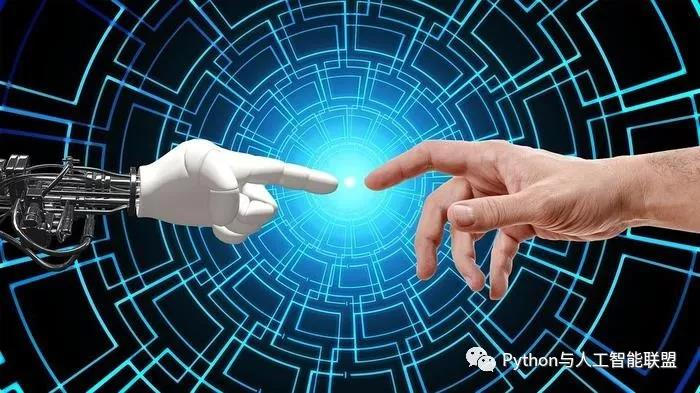
\includegraphics[width=0.75\textwidth]{AI20191218123051.jpg}
%   \label{AI20191218123051}
%\end{figure}
%AI20191218122945.jpg
%AI20191218123051.jpg
%%%%%%%%%%%%%%%%%%%%%%%%%%%%%%%%%%%%
%\begin{itemize}
%\item AI的定义及其研究目标
%\item AI的产生与发展
%\item AI研究的基本内容
%\item AI研究的不同学派
%\item AI的主要研究和应用领域
%\item AI近期发展分析
%\item 我国智能科学技术教育体系
%\end{itemize}
%%%%%%%%%%%%%%%%%%%%%%%%%%%%%%%%%%%%%%%%%%
\begin{figure}[H]
\centering
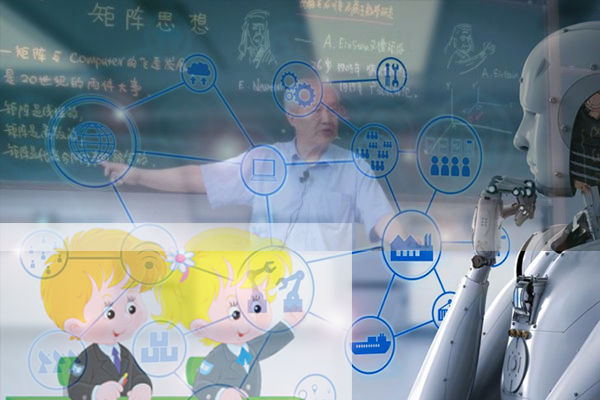
\includegraphics[width=0.6\textwidth]{AI191218001.jpg}
\label{AI191218001}
\end{figure}
%%%%%%%%%%%%%%%%%%%%%%%%%%%%%%%%%%
\begin{tcolorbox}[colback=white!50, colframe=orange!50, title=无名氏]
\begin{center}
   传承是无法避免的,对机器也是可以这么要求的.\hfill
\end{center}
\end{tcolorbox}
%%%%%%%%%%%%%%%%%%%%%%%%%%%%%%%%%%%%
\section{AI的定义及其研究目标}
%%%%%%%%%%%%%%%%%%%%%%%%%%%%%%%%%%%%
\subsection{AI的定义及其研究目标}
\begin{itemize}
\item 目前还没有 形式化定义

\item 一般解释: 人工智能就是用人工的方法在机器(计算机)上实现的智能,或称机器智能.

\item 无形式化定义的理由在于人工智能的严格定义依赖于对\uwave{智能}的定义: 即要定义人工智能,首先应该定义智能,  但智能本身也还无严格定义.
\end{itemize}
\begin{mydef}{人工智能-宋士吉}{1}
人工智能是研究、开发用于模拟、延伸和扩展人的智能的理论、方法、技术及应用系统.
\end{mydef}
因此,先对人类的自然智能进行讨论. \uwave{研究思路就是用人工智能逼近自然智能}.
%%%%%%%%%%%%%%%%%%%%%%%%%%%%%%%%%%%%
\subsection{何谓智能(自然智能)}
\begin{itemize}
\item 自然智能:指人类和一些动物所具有的智力和行为能力.

\item 人类的自然智能(简称智能):指人类在认识客观世界中, 由思维过程和脑力活动所表现出的综合能力.

\item 人类大脑如何实现智能: 不是很清楚人类大脑的信息处理机制和运行机理. 简单来说, 一个人可能在识别图片的时候由于各种劳累和马虎, 在这个数据集的错误率高于机器.
但是只要你去和它谈任何一个图片它所理解的东西, 比如一个苹果, 你都会震惊于其信息之丰富, 不仅包含了真实苹果的各种感官, 还包含了关于苹果的各种文学影视, 从夏娃的苹果, 到白雪公主的苹果.
应该说, 人类理解的苹果更加接近概念网络里的一个节点, 和整个世界的所有其它概念相关联,  而非机器学习分类器里的 $n$个互相分离的高斯分布(机器需要辨识苹果、树、草地和人等).
       大脑的化学反应的变化可以改变行为; Charles Robert Darwin 说: 人和高等动物, 显然只有程度上的区别, 种类上别无二致. 神经科学认为的一个假设是: 认知能力的提高跟大脑随着进化越变越大有关系.
\item 实现智能的两大难题之一: 宇宙起源和人脑奥秘; 然而, 我们对人脑奥秘知之甚少.

\item 目前已知关于人脑的知识

      人脑结构: $10^{11}-10^{12}$量级的神经元, 分布并行;

      人脑功能: 记忆、思维、观察、分析 等.

      脑结构的三个不同层面: \uwave{区域层面、细胞结构层面和分子层面}.

      \ding{172} 大脑皮层位于大脑的外部, 有点像一张覆盖在大脑其他部分之上皱巴巴的大抹布.
      人类大脑和其他灵长类动物大脑在体积上的差异, 主要是皮层增大所致.
      大脑皮层是高度关联的, 在大脑的所有连接中, 75\%位于皮层之内, 仅有25\%是通往大脑其他部分和神经系统的输入输出连接.

      \ding{173}\textbf{新皮层}是大脑皮层中较晚进化出来的区域, 它负责感官知觉、发出运动指令、进行空间推理和有意识思维, 也是智人语言产生的地方.
      解剖学将新皮层分为四个脑叶:\uwave{额叶、顶叶、颞叶和枕叶}. 对包括人类在内的灵长类动物而言, 新皮层大得异乎寻常.
      刺猬的新皮层占大脑重量的16\%, 夜猴(一种小型猴子)占46\%, 黑猩猩占76\%. 人类新皮层所占的比例则更大.
    \begin{figure}[H]
    \begin{center}
    \quad\quad\quad
    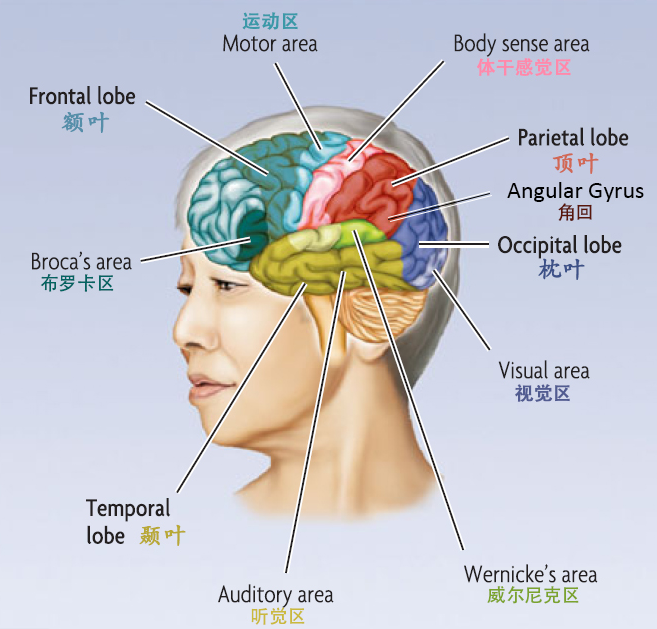
\includegraphics[width=0.45\textwidth]{Brocas2020012801.png}
    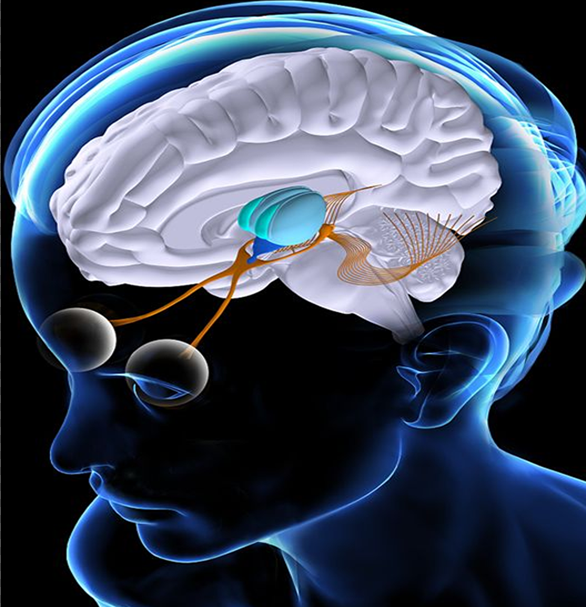
\includegraphics[width=0.416\textwidth]{Brocas2020012802.png}
    \end{center}
    \label{Brocas2020012801}
    \end{figure}
      Michael S. Gazzaniga认为新皮层枕叶包括初级视觉皮层, 也叫纹状皮层. 黑猩猩的纹状皮层占整个新皮层的5\%, 人类的纹状皮层只占2\%, 低于预期值.

      生物神经网络最基本的结构特点是多层, 无论是视觉, 听觉, 我们说基本的神经回路都有层级结构, 而且经常是六层. 这种纵深的层级, 对应的编码原理正是从具体特征到抽象特征的层级编码结构.
      最有名的莫过于祖母细胞, 这一思路直接催生了以 CNN 为代表的深度学习. 从图\ref{Glutamine013001}中的右侧子图可以看出,尼氏染色主要染的是细胞体,而高尔基染色主要染的是树突。
    \begin{figure}[H]
    \begin{center}\quad
    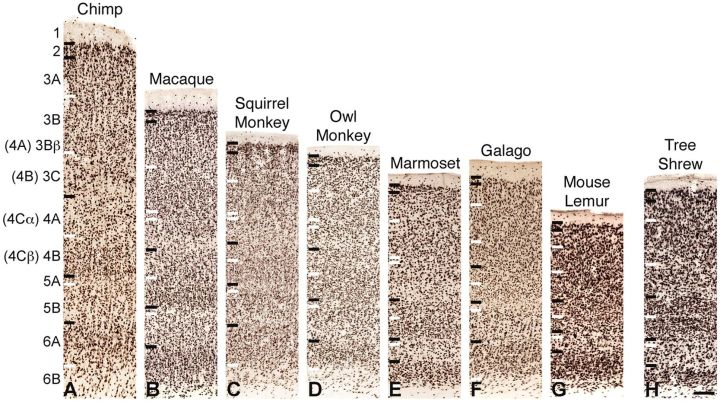
\includegraphics[width=0.44\textwidth]{15339cf86b99167476hd.jpg}
    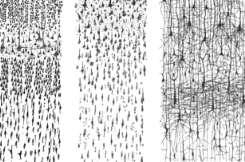
\includegraphics[width=0.4\textwidth]{7ce83064897d1hd.PNG}
    \end{center}
    \caption{灵长类动物的初级视觉皮层分层结构,从左至右分别为黑猩猩,猕猴,松鼠猴,猫头鹰猴,狨猴,婴猴,狐猴,树鼩; 人脑的视觉皮层(尼氏染色);中:人脑的运动皮层(尼氏染色);右:半个月大婴儿的皮层(高尔基染色)}
    \label{Glutamine013001}
    \end{figure}

在进入学龄期这个时期后(7-12-18), 人的脑容量都能达到正常水平. 即使人与人之间在脑容量和褶皱结构有细微差异, 这种差异也不影响智力水平. 不过,这段时期脑内部各个功能区的灰质白质比例, 却的确开始发生很大变化.
总体来讲,这段时期人的脑灰质占比是不断缓慢下降的,而白质占比则不断增高.
    \begin{figure}[H]
    \begin{center}\quad
    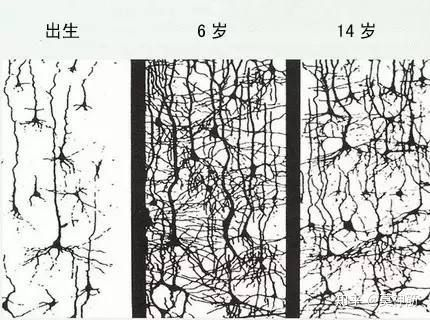
\includegraphics[width=0.44\textwidth]{Nao20200204083453.jpg}
    \end{center}
    \caption{不同时期脑部神经细胞密度}
    \label{Glutamine013001}
    \end{figure}

%%%%%-----------------------------------------------
\paragraph{动物在做决定时如何利用环境}
2020年3月发表在的《神经元》(\href{https://www.cell.com/neuron/fulltext/S0896-6273(20)30061-1}{cell: Neuron-Context-Dependent Decision Making in a Premotor Circuit})杂志上 的一项研究发现, 这种利用环境的能力与老鼠大脑中一个被称为前外侧运动皮层(ALM)的区域, 以前人们认为它主要指导和计划运动. \index{前外侧运动皮层}
这一发现为大脑非凡的决策能力提供了新的视角.
灵活的决策是理解周围环境的关键工具; 所处环境的使用允许决策者通过考虑上下文环境来对相同的信息做出不同的反应.
“环境相关的决策是人类高级认知功能的基石, ”神经学家Michael Shadlen博士说. “就像我们今天的研究一样, 在老鼠大脑的运动区域观察这个过程, 让我们更接近于了解脑细胞和神经回路层面的认知功能. ”

\begin{newexam}
  “如果有人在冷清的街道上不舒服地站在我身边, 我可能会试图逃跑, 但如果同样的事情发生在拥挤的地铁车厢里, 我就不会感到这样的危险, ”神经学家和第一作者郑(赫伯特)吴博士说. “我搬家或不搬家的决定取决于我所处的环境;从而为我所做的选择提供一个理由. ”
\end{newexam}

\begin{newexam}
研究小组调查了大脑中几个专门处理和整合感觉信息的区域, ALM关键区域是运动皮层的一部分.
先前的实验表明, ALM有一个相对简单的工作: 引导老鼠舌头和面部肌肉运动.
基于这一认识, 研究人员设计了一项新的实验, 要求老鼠利用舌头和嗅觉系统做出灵活的决定, 而嗅觉系统是嗅觉的向导. 在实验中, 一只老鼠第一次闻到一种气味.
老鼠必须记住这种气味, 因为在短暂的停顿之后, 研究人员将另一种气味喷到老鼠的鼻孔上. 如果两种气味相同, 老鼠必须舔左边的管子才能得到水. 如果两种气味不同, 它必须向右舔一根管子.
\end{newexam}

先前在这类“延迟匹配样本”测试中所做的工作, 会让人认为老鼠会利用大脑中专门负责嗅觉的区域来决定舔食的方式. 来自这些区域的大脑活动记录似乎证实了这一机制.
“根据这些记录, 我们可以想象, 当老鼠闻到第二种气味时, 这些大脑区域就有了答案, ”Shadlen博士说. “剩下要做的就是把这个答案传递给大脑的运动系统, 从而产生对左右舔的适当反应. ”
如果是这样, 那么运动区域就不应该起作用, 直到提供了第二种气味, 而老鼠决定这两种气味是相同的还是不同的. 吴博士想出了一个聪明的方法来验证这个预测. 他关掉了老鼠的ALM, 直到发出第二种气味, 然后及时打开ALM, 让老鼠得到答案.
按照标准的观点, 老鼠应该不会被这种操作所影响, 因为它们的嗅觉系统仍然完好无损. 相反, 他们在这项任务中受到了损害. ”Michael Shadlen, 医学博士, 研究论文的合著者, 哥伦比亚大学祖克曼研究所神经学家
吴博士说:“我们的研究结果表明, 我们需要ALM来解决两种气味是否匹配的问题, 然后再决定舔到哪里, 这促使我们重新思考大脑是如何做出这些决定的. ”
ALM与气味感知无关.

\begin{newexam}
吴博士仔细观察了ALM中的脑细胞. 他在离大脑表面很近的地方发现了一种新的神经元, 这种神经元对第一种气味有反应. 它将这些信息放在手边, 直到接收到第二种气味.
为了探索这一意想不到的结果, 研究小组求助于理论神经学家Ashok Litwin-Kumar博士, 以调查多种可能解释ALM作用的潜在机制.
“传统观点认为, 动物的嗅觉大脑区域应该自己处理气味, 然后将信息反馈给ALM, 后者将指导舌头, ”Litwin-Kumar博士说. “但数据告诉我们一个不同的故事;第一种气味作为一种上下文线索, 刺激ALM, 然后通过决定舔第二种气味的方式来表明这种关系. ”
\end{newexam}

今天的发现, 虽然集中在ALM上, 但对于如何让科学家对整个大脑功能有更大的理解是很重要的.
“最终, 我们想要阐明解释简单行为的基本原理, 但这也为深入了解人类的高级认知功能提供了思路, ”Shadlen博士说. 要实现这个目标, 关键的一步是用生物学和数学的语言把有关神经元、回路和行为的知识结合起来. 这个合作项目凸显了这一战略的前景. ”

%%%%%-----------------------------------------------
\paragraph{分布强化学习的AI研究}
DeepMind与哈佛大学的研究人员受最近关于分布强化学习的AI研究启发, 提出了一种基于多巴胺的强化学习的方法 \cite{DabneyKurth-Nelson2020-9599}.
和AI系统类似, 大脑不是以“平均值”的方式预期未来可能的回报, 而是以“概率分布”的方式来预期, 从而证明大脑中存在“分布强化学习”. 大脑进行强化学习, 类似于顶级AI算法
“大脑中的多巴胺是一种代表惊讶(surprise)的信号. ” Will Dabney说: “当情况好于预期时, 就会释放出更多的多巴胺. ”

生物神经系统包含种类丰富的抑制型神经元, 它们往往在生物神经网络起到调控功能, 如同控制信息流动的路由器, 在合适的时候开启或关闭某个信号.
当下的 AI 直接用 attention 的机制 (把注意力集中放在重要的点上, 而忽略其他不重要的因素. 重要程度的判断取决于应用场景和主题的认识感知程度. 根据应用场景的不同, Attention分为空间注意力和时间注意力, 前者用于图像处理, 后者用于自然语言处理), 或者 LSTM 里的输入门来调控是否让某个输入进入网络, 其它一点类似路由器的作用, 但是种类和形式的多样性远不及生物系统. 皮层内的神经元都采取簇状结构, 细胞之间不是独立的存在, 而是聚集成团簇, 犹如一个微型的柱状体. 这些柱状体成为信息传输的基本单元. 图\ref{Glutamine013001}的右侧子图是初级感觉皮层(左)和初级运动皮层(右)的分层结构, 可以看到初级感觉皮层的第四层最厚, 而初级运动皮层的第四层特别薄.
    \begin{figure}[H]
    \begin{center}\quad\quad\quad
    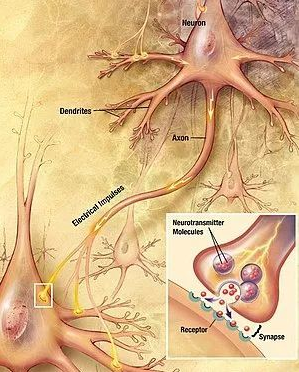
\includegraphics[width=0.355\textwidth]{Glutamine013001.PNG}
    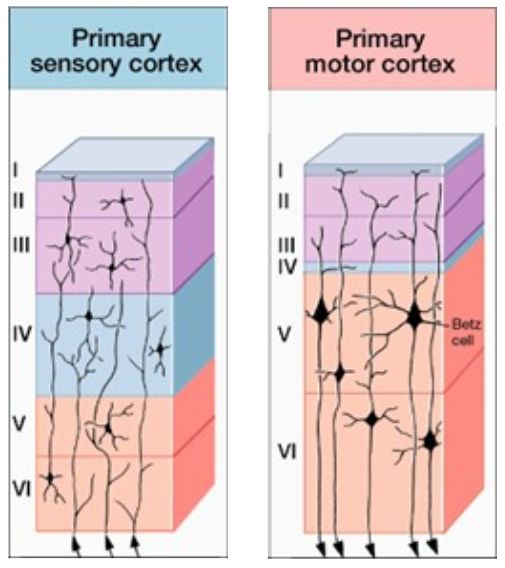
\includegraphics[width=0.4\textwidth]{sjpc4792a5d1hd.jpg}
    \end{center}
    \caption{兴奋型和抑制型神经元; 皮质小柱}
    \label{Glutamine013001}
    \end{figure}

  意识可以理解为自我对自我本身的感知.  关于意识的起源, 已经成为一个重要的神经科学探索方向, 意识与多个脑区协同的集体放电相关(The controversial correlates of consiousness – Science 2018).  但是, 关于意识的一个重大疑团是它对认知和智能到底有什么作用, 还是一个进化的副产物.

  人类大脑海马区神经元放电峰值频率500Hz, 以此推断人类大脑最大计算频率为500hz, 而现在普通电脑的cpu运算也是3.0ghz 以上, 而且还是4核芯, 每秒理论运算次数达到了惊人的120亿次, 运算速度已经远远超过人类大脑. 机器学习认知方面 当下展示出来的智力水平最多也就是3-5岁的小孩子, 计算效率存在差异.
\item 对智能的严格定义有待于人脑奥秘的揭示, 进一步认识.
\end{itemize}
%%%%%%%%%%%%%%%%%%%%%%%%%%%%%%%%%%%%
\subsection{认识智能的几种理论}
\begin{itemize}
\item 思维理论

     智能来源于思维活动, 智能的核心是思维, 人的一切知识都是思维的产物. 可望通过对思维规律和思维方法的研究, 来揭示智能的本质.
\item 知识阈值理论

     智能取决于知识的数量及其可运用程度. 一个系统所具有的可运用知识越多, 其智能就会越高.
\item 进化理论

     是美国MIT的Brooks在对人造机器虫研究的基础上提出来的. 智能取决于\uwave{感知}和\uwave{行为}, 取决于对外界复杂环境的适应, 智能不需要知识、不需要表示、不需要推理, 智能可由逐步进化来实现.
\end{itemize}
%%%%%%%%%%%%%%%%%%%%%%%%%%%%%%%%%%%%
\subsection{智能的层次结构}
各种理论的观点不一致, 从层次结构来说
\begin{itemize}
\item 高层智能: 以大脑皮层(抑制中枢)为主, 主要完成记忆、思维等活动.
\item 中层智能: 以丘脑(感觉中枢)为主, 主要完成感知活动.
\item 低层智能: 以小脑、脊髓为主, 主要完成动作反应活动.

\end{itemize}
\begin{remark}
\textit{不同观点在层次结构中的对应关系}: \textbf{高层智能}: 思维理论、知识阈值理论、进化理论 . 对应基础层. \textbf{中层智能}和低层智能分别对应技术层和应用层.
\end{remark}
%%%%%------------------------------------------
\begin{think}
  大脑是深度学习吗? \index{深度学习}
\end{think}
\begin{remark}
大脑是一个复杂得难以想象的东西, 它把许许多多结构不同的东西包括在内, 而我们对大脑的了解还太少; 大脑是不是深度学习, 我们还给不出确定的答案. 大脑总体来说不是深度学习, 不过其中的某一些子模块可以用深度学习来描述, 或者是部分符合深度学习的, 比如视觉皮层就有深度层次化的特征表征, 即便这些表征不都是学习得到的;视觉皮层也是深度学习的研究中重要的灵感来源.
\end{remark}
%%%%%%%%%%%%%%%%%%%%%%%%%%%%%%%%%%%%
\subsection{智能包含的能力}
\begin{itemize}
\item 感知能力: 通过感知器官感知外界的能力. 是人类获得外界信息的基本途径, 其处理方式有以下两种:

     \qquad$\bullet$ 感知-动作方式: 对简单、紧急信息.

     \qquad$\bullet$ 感知-思维-动作方式: 对复杂信息.
\item 记忆能力

      \textbf{记忆}: 对感知到的外界信息和由思维产生的内部知识的存储过程.

\item 思维能力
         \textbf{思维}: 对已存储信息或知识的本质属性、内部知识的认识过程.

         思维方式:
         \begin{itemize}
           \item 抽象思维(逻辑思维): 根据逻辑规则对信息和知识进行处理的理性思维方式.
           \begin{example}
             逻辑推理等.
           \end{example}
           \item 形象思维(直感思维): 基于形象概念, 根据感性形象认识材料对客观现象进行处理的一种思维方式.
           \begin{example}
             图像、景物识别等.
           \end{example}
           \item 灵感思维(顿悟思维): 是一种显意识和潜意识相互作用的思维方式.
           \begin{example}
             因灵感而顿时开窍.
           \end{example}
         \end{itemize}

\item 学习和自适应能力
      \begin{itemize}
       \item 学习: 是一个具有特定目的的知识获取过程, 是人的一种本能. 不同人的学习方法、能力不同.
       \item 自适应: 是一种通过自我调节适应外界环境的过程, 是人的一种本能. 不同人的适应能力不同.
      \end{itemize}
\item 行为能力: 是人们对感知到的外界信息作出动作反应的能力.
     \begin{itemize}
       \item 信息来源: 由感知直接获得的外界信息,  经过思维加工后的信息.
       \item 实现过程: 通过脊髓来控制(来自四肢和躯干的各种感觉冲动都是通过脊髓的\uwave{上行纤维束来传导}, 即传导面部以外的痛觉、温度觉和粗触觉的脊髓丘脑束、传导本体感觉和精细触觉的薄束和楔束等,以及脊髓小脑束的小脑本体感觉). 由语言、表情和体姿等来实现.
    \end{itemize}
\end{itemize}
%%%%%%%%%%%%%%%%%%%%%%%%%%%%%%%%%%%%
\subsection{何谓人工智能?}
%%%%%%%%%%%%%%%%%%%%%%%%%%%%%%%%%%%%
\begin{tcolorbox}[colback=white!50, colframe=orange!50, title=UC Berkely人工智能系统中心创始人兼计算机科学专业教授Stuart Russell]
\begin{center}
   \textbf{人工智能}是研究\uwave{让计算机展现出智慧}的方法. 计算机获得正确方向后就可以高效工作, 这里的正确的方向意味着最有可能实现目标的方向(术语就是最大化效果预期).
   人工智能需要处理的任务包括\uwave{学习、推理、规划、感知、语言识别和机器人控制}等.\hfill
\end{center}
\end{tcolorbox}
%%%%%%%%%%%%%%%%%%%%%%%%%%%%%%%%%%%%

\textbf{标志事件}:AlphaGo基于人工智能的增强技术和深度学习技术,战胜了李世石. 该技术利用大量的数据来训练神经网络, 从而对新数据做出预测行为.

     谷歌旗下的多款其他产品, 如地图、照片和邮箱等产品都开始利用这种技术增强用户体验; 谷歌翻译也将引入这种技术.

     引入深度学习技术的机器翻译软件, 有望达到人工翻译的水准(AlphaGo的改良版AlphaGo Zero使用了新一代的阿法元, 完全从零开始, 不需要任何历史棋谱的指引, 更不需要参考人类任何的先验知识, 完全靠自己一个人强化学习和参悟, 棋艺增长远超阿法狗, 目前的战绩是百战百胜, 击溃阿法狗的记录是100:0).

     Google翻译尝试在部分功能上使用深度学习技术,
     \begin{example}
       利用摄像头即时取词翻译, 这相当于同声传译. 在国内, 微信、QQ等都能取词翻译.
     \end{example}
\begin{remark}
  人工智能是一门专业性很强的计算机科学, 随着各大技术公司和学界的不懈努力, 这项技术未来会惠泽大众, 会给生活带来实实在在的好处.
\end{remark}

\textbf{对人工智能的常见误解}
\begin{itemize}
\item 「人工智能是一个特定技术」. 例如在二十世纪八十年代到九十年代, 人们经常将人工智能与基于规则的专家系统混为一谈. 现在则是将人工智能经常会与多层卷积神经网络混淆. 这有点像把物理和蒸汽机的概念搞混了. \uwave{人工智能探究如何在机器中创造智能意识}, 不是研究中产生的任何特定技术.
\item 「人工智能是一个特定类别的技术方法」. 例如, 经常有人用符号化或逻辑化的方法将人工智能与「其他方法」相互比较, 如神经网络和遗传编程. 人工智能不是一种方法, 它是一个课题. 所有这些方法都是在对人工智能进行研究的产物.
\item 「人工智能是一小群研究者的方向」. 这个误解与前几个错误有关. 一些作者\uwave{使用「计算智能」来指代几个特定的研究者群体, 如研究神经网络, 模糊逻辑和遗传算法的研究者}. 这是非常片面的, 这种分类方式让人工智能的研究陷入孤立境地, 研究成果不能得到广泛的注意.
\item 「人工智能只是算法」. 严格说来不算是误解, 人工智能的确包含算法(也可粗略定义为程序), 它也包含计算机中其他的应用. 当然, 人工智能系统需要处理的任务相比传统算法任务(比如排序、算平方根)复杂得多.
\end{itemize}
综合各种不同观点, 仅从\textbf{能力}和\textbf{学科}两个方面讨论人工智能:
\begin{itemize}
\item 能力方面: 人工智能就是用人工的方法在机器(计算机)上实现的智能, 或称机器智能.
\item 学科方面: 是一门研究如何构造智能机器或智能系统, 以模拟、延伸和扩展人类智能的学科.
\item Turing测试: 如图\ref{AI:turingFig1}所示. 能分辨出人和机器的概率小于50\%.
\begin{remark}
  Turing测试存在的问题: 仅反映了结果的比较, 不涉及思维过程, 没指出是什么人.
\end{remark}
\end{itemize}

---Turing测试(图{AI:turingFig1})
\begin{figure}[htbp]
\begin{center}
\begin{tikzpicture}[font={\sf \small}]
\def \smbwd{2cm}
\def \smbwe{4cm}
\node (Gei) at (2,0) [draw, process,minimum width=\smbwd, minimum height=0.5cm] {图灵测试}; % 给
\node (ZCR1)[align=center,below=2cm of Gei,yshift=0cm] {
\includegraphics[width=0.25\textwidth]{turing120191201.png}};
\node (TZCR1)[align=center,below=1.8cm of Gei,yshift=-4.5cm] {测试主持人};
\node (JQ1)[align=center,left=2cm of Gei,yshift=0cm] {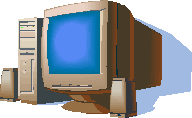
\includegraphics[width=0.25\textwidth]{turing220191201.png}};
\node (TJQ1)[align=center,left=2.3cm of Gei,yshift=-1.85cm,xshift=0.25cm] {被测机器};
\node (BCR1)[align=center,right=2cm of Gei,yshift=0cm] {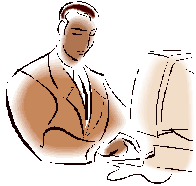
\includegraphics[width=0.25\textwidth]{turing320191201.png}};
\node (TBCR1)[align=center,right=2.3cm of Gei,yshift=-1.85cm] {被测人};
\draw[thick,blue,<->] (0,-5) parabola (-3,-1.5);
%加上bend at end 属性, 就会以终点为抛物线顶点.
\draw[thick,blue,<->] (4,-5) parabola (7,-1.5);
%%\draw[green] (-0.5,3) parabola bend (0,0) (2,3);%相当于画了两条顶点相同抛物线,
\end{tikzpicture}
\end{center}
\caption{图灵测试}
\label{AI:turingFig1}
\end{figure}
%%%%%%%%%%%%%%%%%%%%%%%%%%%%%%%%%%%%
\subsection{人工智能的近远期目标}
\begin{itemize}
\item 远期目标: 揭示人类智能的运行机理, 用智能机器去模拟、延伸和扩展人类的智能.
              涉及到\uwave{脑科学、认知科学、计算机科学、系统科学、控制论等多种学科的共同发展}.

\item 近期目标: 研究如何使现有的计算机更聪明, 即使它能够运用知识去处理问题, 能够模拟人类的智能行为.

\item 相互关系: 远期目标为近期目标指明了方向. 近期目标则为远期目标奠定了理论和技术基础.
\end{itemize}
%%%%%%%%%%%%%%%%%%%%%%%%%%%%%%%%%%%%
\subsection{人工智能对计算机科学的影响}
人工智能时代的来临, 给计算机体系结构的创新带来了新的黄金时代, 挑战的同时也要抓住机遇.

在过去的 50 年间, 人工智能的发展经历了三次起伏, 其中的三大关键因素便是\textbf{算法、大数据和算力}.
而在当下的第三次浪潮中, 软件和硬件的融合成为新的趋势, 其中 AI芯片更是成为了此次浪潮中极为重要的因素. 传统意义上的软件公司如 Facebook、亚马逊, 以及中国的互联网企业都开始涌入这一领域.
这一形势下, 呈现出百花齐放的形势, 让硬件研发存在更多的可能性.
具体而言, 可以探索的三个大方向:

一、\Circled{异构计算}. AI 时代没有哪一个单独的芯片能够做到一统天下, 如 CPU、GPU、FPGA 这些不同的通用芯片, 各有其优势, 未来可能需在同一个平台上使用不同的芯片. 研究异构计算方法, 提高高性能分布式系统的训练效率.

二、\Circled{专用 芯片}. 从谷歌在 2017 年发布的第一款 ASIC TCP——TPU, 到阿里前不久发布的平头哥含光 900芯片, 这些专用的芯片相比通用芯片的优势非常明显. 都是为特定的场景定制, 功耗低、成本低以及性能优.

三、\Circled{围绕存储做新架构探索}. AI 时代对存储的带宽容量的要求非常高, 计算过程中将数据从存储搬到计算单元、再从计算单元搬回存储中所需的容量和性能损失远远超过做计算本身. 因此, 当下 AI 硬件创新面临的一个很重要的挑战, 就是存储墙. 有两个探索方向:

方向 一是利用 3D 堆叠技术解决未来计算中的存储带宽问题. AMD 于 2015 年发布的 Fiji 核心便是这一思路的产物, 其可以直接用 Fiji GPU 来加速 DNN, 性能大幅提高. 现在, 几乎所有 AI 芯片公司都会沿用这一思路, 考虑在芯片训练中使用这种 HBM(高带宽存储器).

方向二是计算存储一体化, 这是未来有可能改变传统的把计算和存储分开的冯·诺依曼架构的一个方向, 并且这种方法不仅仅改变计算机体系结构, 还能在材料、底层半导体技术上做更新. 其中一个比较有趣的工作便是 ReRAM 技术, 能够让计算和存储发生在同一个地方, 而不需要做数据的搬移, 节省的能耗和提高的性能非常多.

AI 时代, 可以探索到计算机体系结构前沿主题, 从底层看, 可以尝试异构计算、3D 堆叠以及计算存储一体化等; 往上看, 则是在应用层做创新.

AI 计算系统体系提出了一致的愿景:未来的 AI 计算应该是分等级的分布式计算系统, 即从云到边缘设备再到终端设备, 让不同等级的数据在不同的地方进行计算和处理, 从「AI in Cloud」变成「AI Everywhere」.
而要实现这一愿景, 还面临着一个难题:计算需求和功耗受限之间的矛盾. 具体到 AI 芯片设计上, 则主要有以下三个主要的挑战:

1) 来自于可编程能力. 也就是说, 随着算法的演进, AI 芯片能够通过编程得到持续改进.

2) 来自于 AI 芯片落地应用处理任务时, 不仅需要处理神经网络, 还需要处理大量常规的计算或经典的信号处理计算.

3) 能耗问题, 尤其是对于边缘设备或者物联网设备而言, 能耗问题非常突出.

为了实现这种超高能效、可编程又具有灵活性的计算, 在过去六七年的时间里已经有了相当多的工作, 主要沿着两个方向努力:一个方向是算法方向, 对神经网络模型进行剪枝、压缩、量化、低位宽化; 另一个方向则是在领域专用的体系结构上的探索, 包括数据粒度、编程和存储模型等.

针对体系架构(尹首一教授等的一系列工作), 其中就包括采用基础的可重构计算架构来做 AI 计算芯片, 主要从 MAC 单元、PE 及 PE 阵列架构三个层面上实现了硬件的可重构能力. 采用这种架构设计出来的芯片, 不仅能够支持灵活的、不同神经网络的编程, 还能极大地降低能耗.
下一阶段, 尝试实现可重构、可编程的体系结构和存储计算一体化(In-Memory Computing)的融合. 「这样才是一个将来能够真正把计算和能效继续推高, 把芯片的适用性和灵活性继续扩大的 AI 芯片解决方案. 」

现在的计算逐渐从云端走向边缘端, 然而边缘端的计算目前还存在很多问题:一方面是移动设备「算不好」; 另一方面则是穿戴设备「算不了」. 而这些问题背后的原因主要还是边缘端的智能计算复杂度太高, 当前的芯片还无法满足这类边缘端计算的需求.
在过去很长一段时间, 国内学术界研究算法和研究硬件的人属于两个完全不同的领域, 各自「井水不犯河水」, 几乎很难一起做研究, 然而随着近几年来智能计算的发展, 尤其是深度学习模型对芯片架构提出了新的挑战和诉求, 计算和芯片二者在研究中结合得越来越紧密.

智能计算按应用领域分为\uwave{云端}和\uwave{边缘端}, 按任务可以分为\uwave{训练}和\uwave{推理}, 这四者可以组成四个象限:\uwave{云端训练、云端推理、边缘推理以及边缘训练}. 而随着目前智能计算走过了从云端训练到云端推理、再到边缘推理的阶段, 下一步可以探索边缘训练, 特别是随着 5G 通信的到来, 将为这一方向的探索带来了更多的机会(中国科学院自动化研究所南京人工智能芯片创新研究院常务副院长程健).

人工智能时代的到来使社会的生产要素发生了根本性变化. 生产力的三要素, 劳动者、劳动对象、劳动资料都在发生巨大变化, 这三要素都跟计算密切相关, 是人工智能计算是未来核心动力.

在农业时代、工业时代, 甚至信息时代, 劳动者没有发生太大的变化, 但是在智慧时代, 自然人和人工智能结合, 对劳动者的生产能力产生了极大的促进, 比如过去受自然环境的影响, 我们用人工去识别图像, 资料, 现在靠人工智能来做, 识别效率得到了成千上万倍的提升; 进入智慧时代, 数据成为重要的劳动对象, 以前的劳动对象, 是一种自然资源, 会在生产过程中, 消耗或转化, 而数据资源使用后仍然存在, 并且又生成了新的数据, 数据资源生生不息; 同时, 计算设备成为了新的劳动资料, 特别是人工智能时代, 劳动资料呈现指数级的需求.

“人工智能计算是未来核心动力, 代表着智慧计算的发展方向”(王恩东). 在人工智能计算中, 由于大场景、大计算需求越来越明显, 用通用芯片进行AI计算可能越来越不实用, 而更多的加速芯片会占据主流. 在这方面, 国内外很多的企业, 像谷歌、亚马逊、Facebook, 中国的BAT、浪潮, 都在AI领域不断的创新. 目前的AI计算服务, 一方面是以云的形式提供, 另一方面以物理服务器的形式提供.

目前, 浪潮在AI服务器领域, 中国市场占比超过50\%, 大部分AI企业使用浪潮服务器进行AI的深度学习和推理训练. 此外, 浪潮也在围绕AI算法优化、框架融合应用等方面持续创新.

人工智能推动了各个行业从信息化向智慧化升级, 提高了社会经济的效率, 并在多个行业引发了新一轮商业模式创新. 如在金融领域, 智能分析系统能够秒级完成人工一年36万小时的合同分析工作; 在制造领域, 一些大型的制造企业已经用智能机器人代替了50\%以上的劳动力. 从宏观来看, 人工智能发展将成为中国经济增长的新引擎, 相关数据显示, 到2035年人工智能领域的经济总量在整体经济的占比将达到20\%.
%%%%%%%%%%%%%%%%%%%%%%%%%%%%%%%%%%%%
\subsection{计算机科学与技术、软件工程、物联网、大数据专业的区别}
\begin{itemize}
\item 计算机科学与技术

计算机科学与技术专业是一个比较传统计算机类专业之一, 特点是注重基础知识结构的构建, 这个专业往往有较为全面的知识结构, 未来的就业面也相对更广一些, 目前很多IT行业的技术研发人员都是该专业毕业的.
不是该专业的人, 如果未来有明确的读研计划或者专业技能提升计划, 可以重点考虑一下计算机科学与技术专业, 未来在就业的方向上也会有更大的选择空间.

\item 软件工程

软件工程专业比较注重学生动手实践能力的培养, 相对于计算机科学与技术专业来说, 软件工程专业的知识结构也有所调整, 会增加一部分关于软件项目管理方面的课程, 更偏向于软件方面的知识.
软件工程专业近些年来的就业情况非常不错, 这与当前软件行业的快速发展有较为直接的关系.

\item 物联网

物联网专业的知识结构分为三大部分. 一、计算机硬件知识; 二、软件开发知识; 三、网络知识.
由于早期物联网领域的产业规模相对较小, 所以早期物联网专业的就业情况不太理想, 很多这个专业的人会选择软件开发领域的相关岗位.
但是, 随着5G的落地应用, 物联网未来的发展前景将非常广阔, 所以目前物联网专业也是热门专业之一.

\item 大数据

大数据专业是新开设的专业之一, 大数据专业在知识结构上与其他传统计算机专业的差别还是比较明显的, 重点增加了统计学相关知识, 同时还会增加一些行业领域的专业知识, 比如经济学、社会学、医学等, 不同高校会根据自身的实际情况来设置具体的课程体系.

\item 催生的新行业
智能制造工程技术人员、工业互联网工程技术人员、虚拟现实工程技术人员、人工智能训练师、连锁经营管理师、供应链管理师、网约配送员、电气电子产品环保检测员、全媒体运营师、健康照护师、呼吸治疗师、出生缺陷防控咨询师、康复辅助技术咨询师、无人机装调检修工、铁路综合维修工和装配式建筑施工员等16个新职业(2020年3月, 人力资源和社会保障部与市场监管总局、国家统计局联合向社会发布).
\end{itemize}
%%%%%%%%%%%%%%%%%%%%%%%%%%%%%%%%%%%%
\subsection{2020年十大科技趋势预测——百度研究院}
\begin{itemize}
\item 趋势1:AI技术已发展到可大规模生产的工业化阶段, 2020年将出现多家"AI工厂", 运用在各行各业帮助产业升级;
\item 趋势2:2020年将会是AI芯片大规模落地的关键年;
\item 趋势3:开源深度学习平台降低了技术开发门槛, 提高了AI应用的质量和效率, 深度学习技术将深入渗透到产业层面, 开始大规模应用;
\item 趋势4:自动机器学习AutoML将大大降低机器学习的门槛;
\item 趋势5: 多模态深度语义理解技术进一步成熟并将得到更广泛应用;
\item 趋势6:自然语言处理技术将与知识深度融合, 面向通用自然语言理解的计算平台得到广泛应用;
\item 趋势7:物联网将在边界、维度和场景三个方向形成突破 (突破云计算中心的边界, 向万物蔓延. 物理世界的时间和空间维度将被拓展. 物联网与能源、电力、工业、物流、医疗、智能城市等更多场景发生融合);
\item 趋势8:智能交通将加速在园区、城市等多样化场景中的落地;
\item 趋势9:区块链技术将以更加务实的姿态融入更多场景, 围绕区块链构建的数据确权、数据安全、数据使用、数据流通和交换等解决方案将在各行各业发挥巨大的作用;
\item 趋势10:量子计算将迎来新一轮爆发, 为AI和云计算注入新活力.
\end{itemize}

2019年3月召开的中央全面深化改革委员会第七次会议上, 审议通过了包括《关于促进人工智能和实体经济融合的指导意见》在内的八份文件, 是国家层面促进人工智能发展的又一份重要指导文件.
会议指出, \uwave{促进人工智能和实体经济深度融合, 要把握新一代人工智能发展的特点, 坚持以市场需求为导向, 以产业应用为目标, 深化改革创新, 优化制度环境, 激发企业创新活力和内生动力, 结合不同行业、不同区域特点, 探索创新成果应用转化的路径和方法, 构建数据驱动、人机协同、跨界融合、共创分享的智能经济形态}.

“\uwave{智能+}”被写入政府工作报告, 人工智能技术对社会的赋能被进一步提高. 在工业经济由数量和规模扩张向质量和效益提升转变的关键期, “智能+”的理念给人工智能等数字技术提供了最广阔的落地空间和回报想象. 通过智能化手段把传统工业生产的全链条要素打通, 可以更好地推动制造业的数字化、网络化和智能化转型, 更能反向助推技术自身的迭代和进步.

$\bullet$ 国产芯片和人工智能双突破

2019年8月, 清华天机AI芯片登上《自然》封面, 这也是中国芯片和人工智能领域第一次登上《自然》杂志. 作为全球首款异构融合类脑芯片, 它让自行车实现“无人驾驶”. 据报道, 天机芯片采用多核架构, 有多个高度可重构的功能性核, 可以同时支持机器学习算法和类脑电路. 从长远来看, 以通用人工智能为目标的“天机芯”, 如果真能实现自己的理想, 它将“无所不能”, 可用于各行各业.

$\bullet$ 人脸识别纠纷走上法庭

2019年9月初, 一款名为“ZAO”的APP火遍全网, 只需在APP中上传一张照片, 就能将自己的脸替换成大明星, 效果几乎以假乱真. 不过很快, 这款APP就因为涉嫌侵犯用户隐私受到争议, 用户上传脸部信息后, 将面临侵权、盗刷等安全风险. 另一边, 11月, 由于被强制要求刷脸入园, 浙江理工大学特聘副教授郭兵把杭州野生动物世界告上法庭, 这也成为国内人脸识别第一案.

$\bullet$ 新方法让机器人学习提速

2019年12月, 《自然》评出2019年度十大杰出论文, 其中包括苏黎世联邦理工学院用\textbf{数据驱动的方法设计机器人软件来训练四足机器人}, 大大提高了机器人的运动能力和学习速度. 新的训练方法利用强化学习, 使机器人学习的速度提升了1000倍, 动作灵活性和速度都大幅增强, 而且踢不倒, 甚至可以从跌倒中翻身站起. 四足机器人在实验室中的小跑速度已经提升了25\%, 在被推倒或滑倒后, 也能获得平衡, 重新站稳.

$\bullet$ 人脸识别国标开跑

人脸识别技术也在争议中探索着符合用户期待又不损害技术发展的治理模式. 在全国信标委生物特征识别分技术委员会换届大会上, 人脸识别技术国家标准工作组正式成立, 人脸识别国家标准制定工作全面启动.
随着人脸识别技术的广泛应用, 引发的问题也不可忽视, 如技术精度等性能标准缺乏导致的仿冒身份、用户授权被盗用等使用安全问题, 人脸信息收集、存储、处理等使用规范欠缺导致的信息泄露安全问题, 数据滥用、隐私保护缺乏规范等伦理问题. 公众也越发关注该技术在安全性上面临的挑战.

$\bullet$ 人工智能和宇宙

《生命3.0》让我们对人工智能和宇宙有了一个新的认识. 作者是美国迈克斯·泰格马克, 麻省理工学院物理系终身教授、未来生命研究所创始人.
%%%%%%%%%%%%%%%%%%%%%%%%%%%%%%%%%%%
\begin{example}
你说一束光有目标吗?
\end{example}
看起来没有, 向什么方向发射, 光就奔向哪个方向啊, 它自己能有啥目标?
但是, 你知道一个现象, 光线射入水中会发生折射. 光的路径不是一条直线, 而是一个折线.
为什么会这样呢?计算之后发现, 因为这样速度最快.
你可以想象一个救生员, 救生员在海滩上奔跑的速度快, 游泳的速度慢, 所以, 如果他要营救一个落水的游客, 最佳路线不是直直地过去, 而是在海滩上多跑一段, 在水里少游一段, 这样虽然看起来走了冤枉路, 但是总体花的时间最短.

同样道理, 光在空气中传播得快, 在水中传播得慢, 所以光会先在空气中多走一段, 再射到水中, 这样, 它到达目的地的速度更快.
你看, 奇怪吧. 光没有生命, 但是它居然会有自己的行动原则, 用最短时间从这一点到达那一点.
所以, 光的目标是什么?那就是在最短时间内到达目的地.
%%%%%%%%%%%%%%%%%%%%%%%%%%%%%%%%%%%%%%%%%%
\begin{figure}[H]
\centering
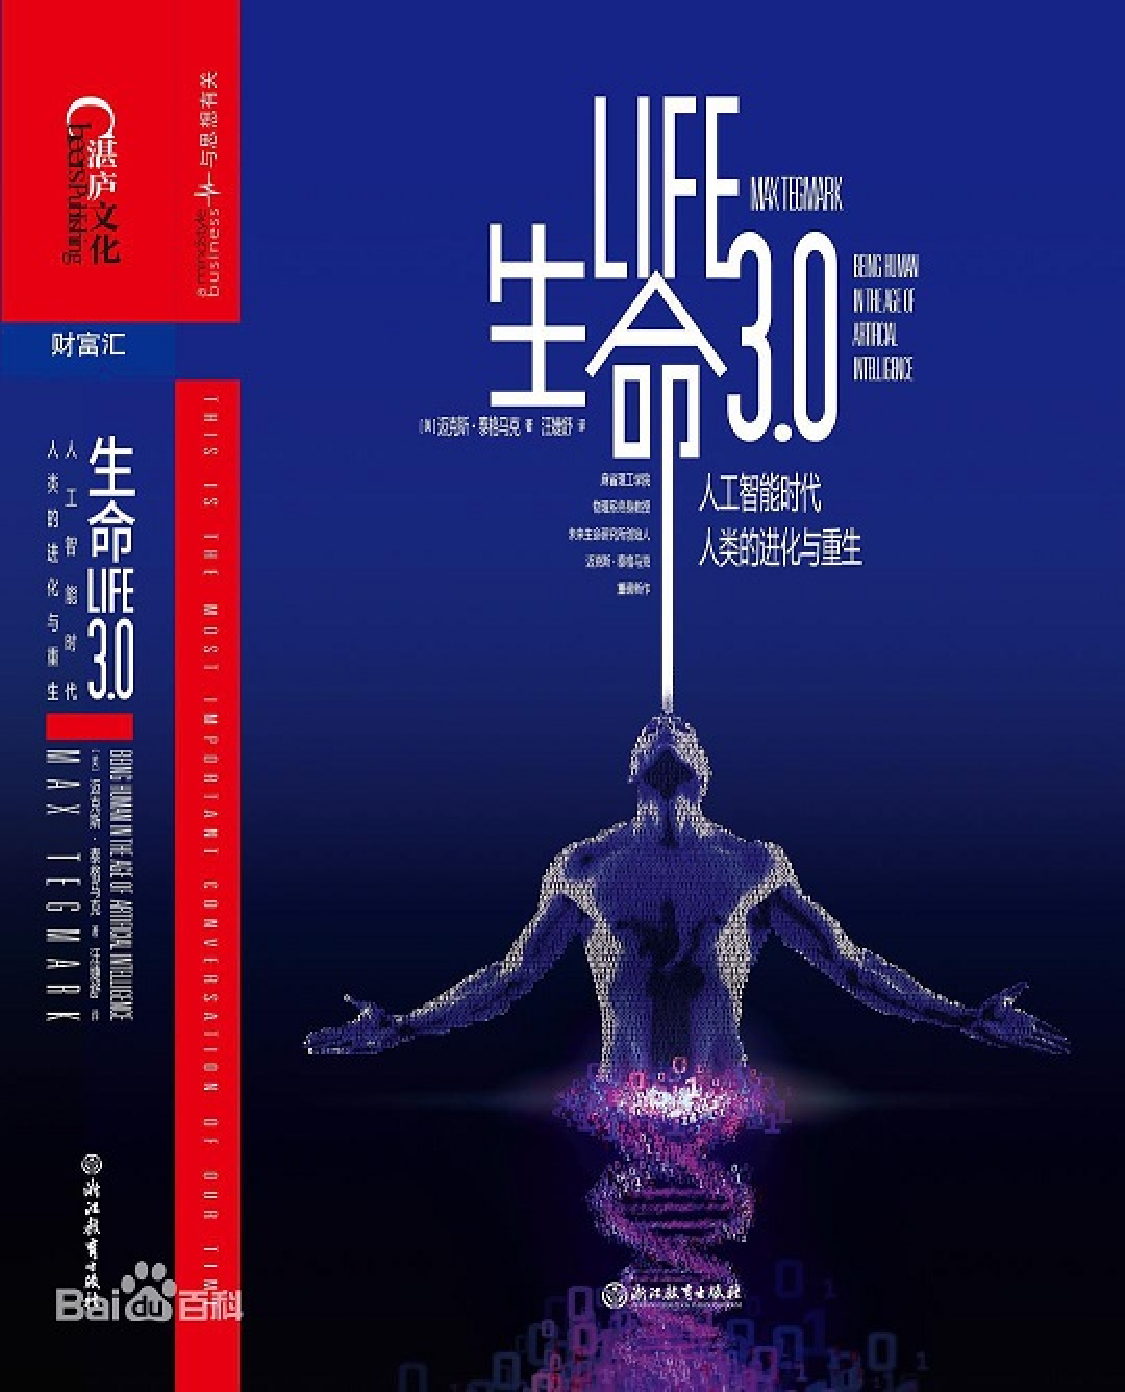
\includegraphics[width=0.46\textwidth]{AI30633d4.pdf}
\caption{生命3.0}
\label{AI30633d4}
\end{figure}
%%%%%%%%%%%%%%%%%%%%%%%%%%%%%%%%%%%%%%%%%%
\begin{figure}[H]
\centering
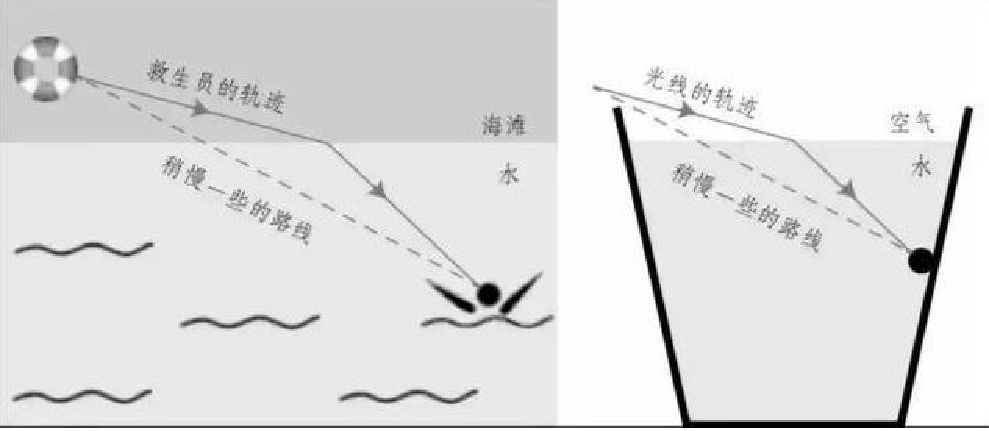
\includegraphics[width=0.76\textwidth]{AIUniverse0102.pdf}
\caption{营救溺水者的最佳路径和光的折射}
\label{AIUniverse0102}
\end{figure}
%%%%%%%%%%%%%%%%%%%%%%%%%%%%%%%%%%%
\begin{example}
那整个宇宙有没有这样的目标呢?
\end{example}
热力学第二定律说\index{热力学第二定律}, 就是追求“熵”的最大化. 简单说就是整个宇宙越来越无序、越来越混乱. 最后整个宇宙归于“热寂”.
\begin{remark}
就是万事万物都扩散成一种无聊而又完美的均质状态.
所有的星星都会熄灭, 所有的秩序都会变成混乱, 所有的地方温度都一样, 再也没有什么值得流动的了, 整个宇宙寂静了.
所以, 可以说宇宙的“目标”, 就是达到热寂.
\end{remark}
%%%%%%%%%%%%%%%%%%%%%%%%%%%%%%%%%%%
\begin{example}
超级人工智能时代, 人类来提供目标.

比如, 我们人类说, 地球太小了, 我们要更大的生存空间, 好, 人工智能就会造一个以恒星为动力源的戴森球.
比如, 人类说, 我想探索真理, 我们想把圆周率尽可能地算下去, 看看它到底有没有尽头, 人工智能就干脆熄灭一个星系的能量, 给人类算圆周率.
人类说, 我要星际旅行, 人工智能就帮你完成这个目标, 过程中耗掉无穷无尽的能量.
这也是一个合作, 人类提供意义和目标, 人工智能提供能力和方法. 这一合作, 宇宙走向热寂的大目标就能越来越快地达成.
\end{example}

\begin{center}
  “\uwave{发展中的问题, 发展中解决}”.
\end{center}
\begin{remark}
  人工智能的终极目标: 机器$\equiv$人.
\end{remark}
%%%%%%%%%%%%%%%%%%%%%%%%%%%%%%%%%%%%
\subsection{美国人工智能计划:2020年度报告}
2020年2月26日, 美国白宫科技政策办公室发布《“美国人工智能计划”:首个年度报告》(下称《报告》). 《报告》由美政府首席技术官克瑞西奥斯与副首席技术官帕克联合签发, 主要从投资AI研发、共享AI资源、消除AI创新障碍等方面, 总结了美政府过去一年在实施“美国人工智能计划”方面取得的重大进展.

《报告》指出, 美政府拥有大量数据、模型及计算资源等重要AI资源. 美政府努力使各界获得高质量、可追溯的AI资源, 支持AI研发, 主要举措包括:①2019年12月, 美政府发布《联邦数据战略2020年行动计划》, 指导各机构开发工具、完善流程, 高效使用数据. ②美国国家科学基金会与DARPA合作开展“实时机器学习”项目, 探索可在连续数据流中学习的硬件与机器学习架构;与联邦公路管理局合作研究隐私技术, 寻求远程访问高速公路数据库;资助加利福尼亚大学及华盛顿大学开发并运营“云银行”(CloudBank), 为计算机科学人员提供公共云. ③美国能源部为国家癌症研究所提供超级计算机, 开发治疗癌症的AI解决方案. 三、消除AI创新障碍《报告》认为, AI仍然处于起步阶段. 美政府发布多项文件以指导制定相关法律、法规及标准, 消除AI创新障碍, 快速推进AI发展, 包括:

\ding{172} 2019年4月, 美国食品药品监督管理局提出针对医疗AI软件的监管框架, 确保这些软件安全有效.

\ding{173} 2019年8月, 美国国家标准技术研究院发布《联邦政府参与开发技术标准与相关工具的计划》, 强调美政府应持续参与AI标准开发活动, 推进可信任AI技术发展.

\ding{174} 2020年1月, 美国运输部发布《确保美国在自动驾驶汽车技术中的领导地位:自动驾驶汽车4.0》文件, 详细阐述了美政府在自动驾驶汽车领域的若干原则. ④2020年1月, 美政府发布监管AI的10项原则, 包括公众信任、公众参与、科学诚信与信息质量等.
%%%%%%%%%%%%%%%%%%%%%%%%%%%%%%%%%%%%
%\subsection{José Luis García Vigil-未来十年预测12/26/2019: Report to Enrique Portillo}
%
%We went to the future ... and we came back to tell you the 5 technologies that will explode in the next decade
%
%Telepresence and brains 'connected to the cloud'. By 2030,  technology will take a leap that can go beyond our imagination.
%Flying cars. Talking robots. Interstellar travel Science fiction has raised scenarios that seemed crazy for decades,  but now are real possibilities thanks to the leaps and bounds of technology.
%Maybe we still don't see cars in the skies,  but there are already several companies with projects in development of flying taxis. Will people ever get to other planetary systems? We do not know,  but there are objects made by humans (the Voyager 1 and Voyager 2 probes,  launched in 1977) that are already in interstellar space,  billions of kilometers from our Sun. And from robots… well,  we should Ask Alexa,  Siri,  Cortana,  Google and even Sophia to see what they think.

%Beyond these achievements,  the power of technology has also extended to more everyday issues: the ‘plague’ of smartphones,  the era of internet connectivity and even electric cars.
%What will we expect by 2030? Experts in the sector tell us about the technologies that will be a trend in the next ten years and that will become as common as a cell phone in hand.
%Fuimos al futuro… y volvimos para decirte las 5 tecnologías que explotarán en la siguiente década
%El Financiero 26/12/2019: Reportaje a Enrique Portillo
%Telepresencia y cerebros 'conectados a la nube'. Hacia 2030,  la tecnología dará un salto que puede ir más allá de nuestra imaginación.
%Autos voladores. Robots parlantes. Viajes interestelares. La ciencia ficción ha planteado escenarios que hace décadas parecían una locura,  pero que ahora resultan posibilidades reales gracias al avance agigantado de la tecnología.
%
%Quizá todavía no vemos coches por los cielos,  pero ya hay diversas compañías con proyectos en desarrollo de taxis voladores. ¿Alguna vez las personas lograrán llegar a otros sistemas planetarios? No lo sabemos,  pero hay objetos hechos por humanos (las sondas Voyager 1 y Voyager 2,  lanzadas en 1977) que ya se encuentran en el espacio interestelar,  a miles de millones de kilómetros de nuestro Sol. Y de los robots… pues habríamos que preguntarle a Alexa,  Siri,  Cortana,  Google y hasta a Sophia a ver qué ‘piensan’.
%Más allá de estos logros,  el poder de la tecnología también se ha extendido a cuestiones más cotidianas: la ‘plaga’ de los smartphones,  la era de la conectividad a internet y hasta los autos eléctricos.
%¿Qué nos deparará hacia 2030? Expertos en el sector nos hablan de las tecnologías que serán tendencia en los siguientes diez años y que se volverán tan comunes como un celular en la mano.
%https://elfinanciero.com.mx/tech/fuimos-al-futuro-y-volvimos-para-decirte-las-5-tecnologias-que-explotaran-en-la-siguiente-decada
%%%%%%%%%%%%%%%%%%%%%%%%%%%%%%%%%%%%
\section{AI的产生与发展}

50多年来, 人工智能走过了一条起伏和曲折的发展道路. 回顾历史, 可以按照不同时期的主要特征, 将其产生与发展过程分为6个阶段.
\begin{itemize}
\item 孕育期(1956年以前);
\item 形成期(1956——1970年);
\item 知识应用期(1970——20世纪80年代末);
\item 从学派分离走向综合(20世纪80年代末到本世纪初);
\item 智能科学技术学科的兴起(21世纪初以来);
\item 深度学习为代表的人工智能技术(2010年以来).
\end{itemize}
%%%%%%%%%%%%%%%%%%%%%%%%%%%%%%%%%%%%
\subsection{AI的产生与发展-孕育期(1956年以前)}
%%%%%%%%%%%%%%%%%%%%%%%%%%%%%%%%%%%%
\paragraph{AI的产生与发展-孕育期(远古——1946年以前)}

自远古以来, 人类就有用机器代替人们进行劳动的的构想: 公元前900多年我国有歌舞机器人流传的记载; 公元前850年古希腊有制造机器人帮助人们劳动的神话传说; 三国时的木牛流马.
\begin{itemize}
\item  亚里斯多德(Aristotle, 公元前384——公元前322): 古希腊伟大的哲学家和思想家, 创立了演绎法. 他提出的三段论至今仍然是演绎推理的最基本出发点.
\item  莱布尼茨(G. W. Leibnitz, 1646——1716): 德国数学家和哲学家, 把形式逻辑符号化, 奠定了数理逻辑的基础.
\item  图灵(A. M. Turing, 1912——1954): 英国数学家, 1936年创立了自动机理论, 自动机理论亦称图灵机, 是一个理论计算机模型.
\item  莫克利(J. W. Mauchly, 1907——1980): 美国数学家、电子数字计算机的先驱, 与他的研究生埃克特(J. P. Eckert)合作, 1946年研制成功了世界上第一台通用电子计算机ENIAC.
\end{itemize}
%%%%%%%%%%%%%%%%%%%%%%%%%%%%%%%%%%%%
\paragraph{AI的产生与发展-孕育期(1956年以前)}
\begin{itemize}
\item  麦克洛奇(W. McCulloch)和皮兹(W. Pitts): 美国神经生理学家, 于1943年建成了第一个神经网络模型(MP模型).
\item  维纳(N. Wiener, 1874—1956): 美国著名数学家、控制论创始人. 1948年创立了控制论, 使得控制论向人工智能的渗透, 形成了行为主义学派. 1954年, 钱学森在McGraw-Hill出版了《工程控制论》.
\item  图灵又于1950年, 发表题为《计算机能思维吗?》的著名论文, 明确提出了“机器能思维”的观点.
\end{itemize}
\begin{remark}
在人工智能诞生之前, 一些著名科学家就已经创立了数理逻辑、神经网络模型和控制论, 并发明了通用电子数字计算机. 为人工智能的诞生准备了必要的思想、理论和物质技术条件.
\end{remark}
%%%%%%%%%%%%%%%%%%%%%%%%%%%%%%%%%%%%
\subsection{AI的产生与发展-形成期(1956--1970年)}
AI诞生于一次历史性的聚会.
\begin{itemize}
\item  时间: 1956年夏季;
\item  地点: 达特莫斯 (Dartmouth)大学;
\item  目的: 为使计算机变得更“聪明” , 或者说使计算机具有智能.

\item  发起人:
      \begin{itemize}
          \item  麦卡锡(J. McCarthy) , Dartmouth的年轻数学家、计算机专家, 后为MIT教授.
          \item  明斯基(M. L. Minsky), 哈佛大学数学家、神经学家, 后为MIT教授.
          \item  洛切斯特(N. Lochester),  IBM公司信息中心负责人.
          \item  香农(C. E. Shannon), 贝尔实验室信息部数学研究员.
      \end{itemize}
\item  参加人:
      \begin{itemize}
          \item  莫尔(T. More)、塞缪尔(A. L. Samuel),  IBM公司.
          \item 塞尔夫里奇(O. Selfridge)、索罗蒙夫(R. Solomonff), MIT.
          \item 纽厄尔(A. Newell), 兰德(RAND)公司.
          \item 西蒙(H. A. Simon), 卡内基(Carnagie)工科大学.
      \end{itemize}
\item  会议结果:

     由麦卡锡提议正式采用了“Artificial Intelligence”这一术语. AI以“推理、 知识” 为重点.
\end{itemize}

\begin{itemize}
\item  心理学小组
    \begin{itemize}
        \item  1957年, 纽厄尔、肖(J.Shaw)和西蒙等人的心理学小组研制了一个称为逻辑理论机(Logic Theory Machine, 简称LT)的数学定理证明程序.
        \item  1960年研制了通用问题求解(General Problem Solving)程序. 该程序当时可以解决11种不同类型的问题, 如不定积分、三角函数、代数方程、猴子摘香蕉、河内梵塔、人—羊过河等.
    \end{itemize}
\item  IBM工程小组

     1956年, 塞缪尔在IBM704计算机上研制成功了具有自学习、自组织和自适应能力的西洋跳棋程序. 这个程序可以从棋谱中学习, 也可以在下棋过程中积累经验、提高棋艺. 通过不断学习, 该程序1959年击败了塞缪尔本人, 1962年又击败了一个州的冠军.
\item  MIT小组
    \begin{itemize}
       \item  1958年, 麦卡锡建立了行动规划咨询系统.
       \item  1960年, 麦卡锡又研制了人工智能语言LISP.
       \item  1961年, 明斯基发表了“走向人工智能的步骤”的论文, 推动了人工智能的发展.
    \end{itemize}
\end{itemize}

其他方面

     \ding{172} 1965年, 鲁宾逊(J. A. Robinson)提出了归结(消解)原理.

     \ding{173} 1965年, 费根鲍姆(E. A. Feigenbaum) 开始研究化学专家系统DENDRAL.
%%%%%%%%%%%%%%%%%%%%%%%%%%%%%%%%%%%%
\subsection{AI的产生与发展-知识应用期(1971--80年代末)}
%%%%%%%%%%%%%%%%%%%%%%%%%%%%%%%%%%%%
\subparagraph{失败的预言}

60年代初, 西蒙预言: 10年内计算机将成为世界冠军、将证明一个未发现的数学定理、将能谱写出具有优秀作曲家水平的乐曲、大多数心理学理论将在计算机上形成并被验证.
%%%%%%%%%%%%%%%%%%%%%%%%%%%%%%%%%%%%
\subparagraph{挫折和教训}
\begin{itemize}
\item  在博弈方面, 塞缪尔的下棋程序在与世界冠军对弈时, 5局败了4局.
\item  在定理证明方面, 发现鲁宾逊归结法的能力有限. 当用归结原理证明两个连续函数之和还是连续函数时, 推了10万步也没证出结果.
\item  在问题求解方面, 对于不良结构, 会产生组合爆炸问题.
\item  在机器翻译方面, 发现并不那么简单, 甚至会闹出笑话. 例如, 把“心有余而力不足”的英语句子翻译成俄语, 再 翻译回来时竟变成了“酒是好的, 肉变质了”.
\item  在神经生理学方面, 研究发现人脑有$10^{11-12}$以上的神经元, 在现有技术条件下用机器从结构上模拟人脑是根本不可能的.
\item  在其它方面, 人工智能也遇到了不少问题. 在英国, 剑桥大学的詹姆教授指责“人工智能研究不是骗局, 也是庸人自扰”. 从此, 形势急转直下, 在全世界范围内人工智能研究陷入困境、落入低谷.
\end{itemize}
%%%%%%%%%%%%%%%%%%%%%%%%%%%%%%%%%%%%

以知识为中心的研究:
\begin{itemize}
\item  专家系统实现了人工智能从理论研究走向实际应用, 从一般思维规律探讨走向专门知识运用的重大突破, 是AI发展史上的一次重要转折.

2020年3月, 日本诺日士钢机集团旗下的Doctor-NET(东京港区)将启动人工智能检测新型冠状病毒的实证试验. 该公司将与中国的AI开发企业北京推想科技合作, 向日本引进在武汉等地使用的新冠肺炎诊断系统.

\item  1972年, 费根鲍姆开始研究MYCIN专家系统, 并于1976年研制成功. 从应用角度看, 它能协助内科医生诊断细菌感染疾病, 并提供最佳处方. 从技术角度看, 他解决了知识表示、不精确推理、搜索策略、人机联系、知识获取及专家系统基本结构等一系列重大技术问题.
\item  1976年, 斯坦福大学的杜达(R. D. Duda)等人开始研制地质勘探专家系统PROSPECTOR.
\end{itemize}

这一时期, 与专家系统同时发展的重要领域还有计算机视觉和机器人, 自然语言理解与机器翻译等. 但直到80年代末,  所有的AI程序都只是“玩具”.

\textbf{新的问题}: 专家系统本身所存在的应用领域狭窄、缺乏常识性知识、知识获取困难、推理方法单一、没有分布式功能、不能访问现存数据库等问题被逐渐暴露出来.
%%%%%%%%%%%%%%%%%%%%%%%%%%%%%%%%%%%%
\subsection{AI的发展-知识深化期(1990-2000年代末)}
以“特征” 为重点

     \ding{172} 1993年, 支持向量机出现.  国内的王国俊教授提出了三I方法.  由于模糊推理与模糊逻辑在模糊控制中有直接的应用, 模糊推理与模糊逻辑的研究受到模糊系统与人工智能学界的广泛关注. 1997年3月在美国召开的国际信息科学联合会议上, 王国俊作了“\uwave{论模糊推理的逻辑基础}”的报告. 这一报告引起了很多与会代表的浓厚兴趣, 并受到前任国际模糊系统协会主席、纽约宾汉顿大学的Klir 教授以及 Turksen等著名教授在内的许多学者高度评价, 克雷顿大学模糊系统研究所所长Mordeson教授还在该校的研究报告中刊登王的全文. 如今这一成果已全文发表于Information Sciences.
       在此基础上, 王提出了模糊推理的三I方法, 于1999年发表于《中国科学》, 全面改进了传统的CRI方法. 2004年7月, 他在美国盐湖城召开的信息科学联合会议上当选为不确定性数学学会副理事长.

     \ding{173} 1992年, 美国控制论专家L. A. Zadeh教授指出:人工神经网络、模糊逻辑、遗传算法、蚁群算法与传统计算模式的区别, 在于它们与人脑对应, 具有在不确定及不精确环境中进行推理和学习的智能计算能力. 除此之外, 粗糙集方法、机器学习方法以及各种随机搜索技术等也被纳入到人工智能的统一框架中, 人工智能技术已在众多应用领域取得了极大的成功.

     \ding{174} 全蕴涵模糊推理机制与模糊规则的启发式生成方法.  模糊控制系统的核心技术是模糊控制器的设计,  模糊控制器的主要组成部分是\uwave{模糊推理机和模糊规则库}. 70 年代 L.A.Zadeh 教授提出的“复合蕴涵规则”方法虽得以广泛应用, 但模糊推理的基本形式FMP问题的合成推理方法求解使用的合成运算缺乏严格的逻辑依据, 模糊推理逻辑基础问题一直受到了科学家和工程师的极大关注, 同时也已取得了一系列有价值的研究成果. 其中以我国前辈数学家王国俊教授提出的“\uwave{全蕴涵模糊推理机制与推理方法}”受到了最为广泛的关注. 该推理方法在模糊推理的每一步运算过程都使用了蕴涵运算, 通过蕴涵算子给出模糊推理最优解的解析形式. 在此工作基础上, 基于不同的蕴涵方式, 我们提出了反向模糊推理机制与模糊推理算法, 给出了模糊取式和模糊拒取式最优解的解析计算公式.

     \ding{175} 模糊知识约简/模糊决策树生成模糊规则的启发式方法.  1982年Z. Pawlak教授提出的粗糙集理论在处理不完整、不一致和不精确数据的问题中取得成功, 目前已经发展成为一种较为成熟的定量分析数学工具, 在机器学习、数据挖掘、模式识别、故障诊断等领域有着广泛的应用. 其主要思想是将模糊相似关系代替粗糙集的等价关系, 引入模糊上、下近似概念, 并提出模糊约简与模糊核的定义, 提出了一种启发式算法能够从初始模糊数据中学习模糊规则, 该算法从真正意义上实现了从模糊数据抽取模糊规则. 项目进一步开展了模糊决策树归纳学习研究, 提出了一种产生模糊决策树的启发式算法, 将粗集核学习与决策树归纳进行结合, 可生成高性能加权模糊规则.

     \ding{176} 基于极限学习机或随机机会约束模型的智能学习方法.  极限学习机方法的前期工作仅适用于解决有监督的机器学习问题, 不能处理标签数据存在缺失的情形. 针对数据标签有缺失且带有分布流形特性的数据, 基于Laplacian矩阵的流形正则化思想学习数据的流形特性, 构造了两步骤学习的统一框架,  将有监督、无监督和半监督极限学习算法纳入其中. 进而项目研究了基于机会约束模型的有监督学习方法与半监督学习方法. 首先建立了基于随机机会约束的鲁棒支持向量非线性回归模型, 将随机约束优化问题转化为二次锥规划问题, 由内点法可实现高效求解, 解决了回归分析中输入数据和输出数据同时受到噪声干扰的问题.
%%%%%%%%%%%%%%%%%%%%%%%%%%%%%%%%%%%%
\subsection{数据智能——发展期(2000-2009年末)}

2006年, Geoffery Hinton提出深度学习, 使得神经网络得以重生.  关于人工智能的每一个进步都是由30年前的一篇阐述多层神经网络的训练方法的论文(Learning representations by back-propagating errors, \cite{RumelhartHinton1986-9415})演变而来, 它为人工智能在最近十年的发展奠定了基础, 但要保持这种进步, 就要面对人工智能严重的局限性.

多伦多市中心一栋高级大厦, 七层是新成立的人工智能研究所Vector Institute的所在地. 研究所的联合创始人乔丹·雅各布(Jordan Jacobs). 该研究所于今年秋天正式成立, 致力于成为全球人工智能中心.  为了拜访杰弗里·辛顿(Geoffrey Hinton)来到多伦多. 他是“深度学习”之父, 正是这个技术让人工智能发展到今天这般炙手可热. 雅各布说:“我们30年后再往回看, 杰弗里就是人工智能(我们认为深度学习就是人工智能)的爱因斯坦. ” 在人工智能领域最顶尖的研究人员当中, 辛顿的引用率最高, 超过了排在他后面三位研究人员的总和. 他的学生和博士后领导着苹果、Facebook和OpenAI的人工智能实验室; 辛顿本人是谷歌大脑(Google Brain)人工智能团队的首席科学家.

事实上, 人工智能在最近十年里取得的几乎每一个成就, 包括语音识别、图像识别, 以及博弈, 在某种程度上都能追溯到辛顿的工作.
Vector Institute研究中心进一步升华了辛顿的研究. 在这里, 谷歌、Uber、Nvidia等美国和加拿大的公司正努力将人工智能的技术商业化. 资金到位的速度比雅各布想象的更快; 他的两个联合创始人调研了多伦多的公司, 发现他们对人工智能专家的需求是加拿大每年培养的人数的10倍.
某种意义上, Vector研究所是全球深度学习运动的原爆点:无数公司靠这项技术牟利, 训练它、改进它、应用它. 到处都在建造数据中心, 创业公司挤满了摩天大楼, 整整新一代学生也纷纷投身这一领域.
%%%%%%%%%%%%%%%%%%%%%%%%%%%%%%%%%%%%
\subsection{数据智能——爆发期(2010-现在)}
\begin{figure}[H]
\centering
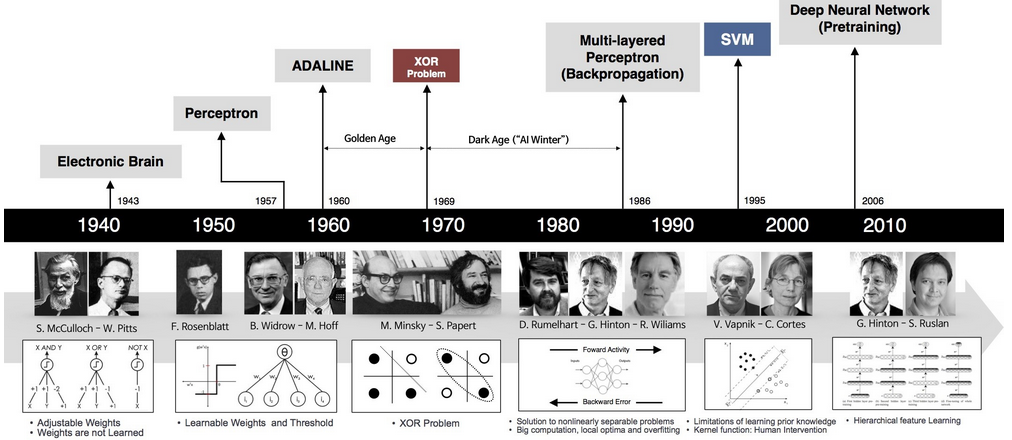
\includegraphics[width=0.86\textwidth]{AIhistory013001.PNG}
\caption{神经网络的发展\href{https://aistudio.baidu.com/}{历史}}
\label{AIhistory01300}
\end{figure}
%%%%%%%%%%%%%%%%%%%%%%%%%%%%%%%%%%
$\blacklozenge$ 2012年, 深卷积神经网络错误率下降到了16\%;在接下来的几年中, 错误率下降了几个百分点. 虽然2012年的突破是“前所未有的组合”, 但大幅量化的改进标志着全行业人工智能繁荣的开始. 到2015年, 研究人员报告说, 软件在狭窄的ILSVRC任务中超出人类能力. 然而, 作为挑战组织者之一的Olga\, Russakovsky在2015年指出, 这些计划只需将图像识别为属于千分之一的图像;人类可以识别更多的类别, 并且(不像程序)可以判断图像的上下文.
\begin{remark}
ILSVRC (ImageNet Large Scale Visual Recognition Challenge)是近年来机器视觉领域最受追捧也是最具权威的学术竞赛之一, 代表了图像领域的最高水平.

ImageNet数据集是ILSVRC竞赛使用的是数据集, 由斯坦福大学李飞飞教授主导\index{李飞飞}, 包含了超过1400万张全尺寸的有标记图片. ILSVRC比赛会每年从ImageNet数据集中抽出部分样本, 以2012年为例, 比赛的训练集包含128\,1167张图片, 验证集包含5E4张图片, 测试集为1E5张图片.

\end{remark}
$\blacklozenge$ 2014年, 超过50家机构参加了ILSVRC. 2015年, 百度科学家因使用不同帐户而被禁止使用一年, 大大超过每周两次提交的指定限制. 百度后来表示, 它解雇了涉及的团队领导, 并建立了一个科学咨询小组.

$\blacklozenge$ 2016年, AlphaGo在一场复杂的围棋比赛中打败了世界冠军, 震惊了计算机科学家们. 它背后的DeepMind团队中的重要成员曾是特南鲍姆的博士后. 特南鲍姆参与了一家创业公司的工作, 这家公司致力于让自动驾驶汽车直观地了解一些基础物理学, 对其他驾驶员的意图也能做出一定的直觉判断, 从而更好地应对从未遇到过的情况, 比如一辆卡车冲到前面或他人强行超车.

$\blacklozenge$ 2016年,  以“学习” 为重点, 出现了\href{http://www.image-net.org/}{ImageNet数据库}. ImageNet项目是一个用于视觉对象识别软件研究的大型可视化数据库. 超过1400万的图像URL被ImageNet手动注释, 以指示图片中的对象;在至少一百万个图像中, 还提供了边界框. ImageNet包含2万多个类别;一个典型的类别, 如“气球”或“草莓”, 包含数百个图像. 第三方图像URL的注释数据库可以直接从ImageNet免费获得;但是, 实际的图像不属于ImageNet. 自2010年以来, ImageNet项目每年举办一次软件比赛, 即ImageNet大规模视觉识别挑战赛(ILSVRC), 软件程序竞相正确分类检测物体和场景.ImageNet挑战使用了一个“修剪”的1000个非重叠类的列表. 2012年在解决ImageNet挑战方面取得了巨大的突破, 被广泛认为是2010年的深度学习革命的开始.辛顿在1986年取得了突破, 他发现反向传播可以用来训练深度神经网络, 即多于两层或三层的神经网络. 但自那以后又过了26年, 不断增强的计算能力才使这一理论得以证实. 辛顿和他在多伦多的学生于2012年发表的一篇论文表明, 用反向传播训练的深度神经网络在图像识别领域打败了当时最先进的系统——“深度学习”终于面世.  神经网络似乎能抓取图像、文字、某人说话的录音、医疗数据等事物, 将它们放到数学家所说的高维矢量空间里, 使这些事物之间的距离远近反映真实世界的一些重要特点. 辛顿相信, 这就是大脑的运作方式.

$\blacklozenge$ 2017年, 38个竞争团队中有29个错误率低于5\%.

$\blacklozenge$ 2017年, ImageNet宣布将在2018年推出一项新的, 更加困难的挑战, 其中涉及使用自然语言对3D对象进行分类. 由于创建3D数据比注释预先存在的2D图像更昂贵, 数据集预计会更小. 这方面的进展应用范围从机器人导航到增强现实.

$\blacklozenge$ 2017年11月前后, 谷歌的AutoML项目发展出新的神经网络拓扑结构, 创建了NASNet, 这是一个针对ImageNet和COCO优化的系统.
据Google称, NASNet的性能超过了以前发布的所有ImageNet性能.

$\blacklozenge$ 2018新一代人工智能院士高峰论坛, 张正友博士加入腾讯并创建 Robotics X 机器人实验室, 他对未来的判断是我们将迎来一个\uwave{人机共生的时代}. 当计算技术、感知技术得到充分应用后, 人机协作、人机共生将有长足的发展.
Robotics X 机器人机器人有6个组成部分, 本体、感知、执行器、动力系统、交互系统、决策. 机器人的未来趋势是自动化、智能化, 要在不确定的环境中自主决策. SLAP范式(SLAP打耳光理论)的提出, 解决机器人的自主决策问题;
传感器和执行器的紧密结合, 在学习和计划模块的帮助下提升能力、做出决策.

自主分为“反应式自主”和“有意识的自主”.  张正友博士提出了“SLAP打耳光理论”实现自主:第一步, 让感知(Sense)和行动(Act)相连, 先得到反应式自主. 在上层规划后, 做到长期自主去规划(Plan), 就是有意识的自主.

第二步, 整个过程中, 机器人还需要不断学习(Learn), 在学习中与外界交互, 与自身交互, 让机器能力越来越强. 这个SLAP范式, 在英文里也有打耳光的意思, 这就是它名字的由来.

当机器人进过SLAP范式进化后, 智能化程度变高, 就有丰富的应用场景, 从操作复杂工艺, 到陪伴和护理儿童与老年人, 到更复杂的人机合作.


机器人本体的研究有六大趋势: \uwave{仿生化, 灵巧操控, 触觉基础, 多机器人协同, 人机协同以及医疗辅助}. 在技术达到人机协同的水平之前, 还有很多的技术研发需求, 技术突破点包括人工智能技术、机器人本体、自动控制、进化学习、情感理解、灵活操控、守护人类, 这对更先进、更智慧的机器人提出了要求. 最终目标是机器人要服务于人.

迁移学习和联邦学习(香港科技大学教授杨强)的提出是针对现代组织机构数据多且是小数据库或者是某一种任务大数据且另一任务小数据情形的智能化学习方案.

第一种方案是\uwave{迁移学习}, 希望像人类一样把以往的任务中学习到的技能运用在新任务中. 迁移学习还可以兼顾可靠性和隐私安全问题. 迁移学习把源领域的模型和任务迁移到新领域, 但迁移学习的本质是找出\uwave{学习中存在的不变量}. 迁移学习中, 定量分析表明模型的浅层比较容易迁移, 理论分析结果可以帮助我们更好地做迁移学习. 例子比如卫星图像识别, 贷款风控不同用户类别间的迁移, 推荐系统的策略迁移, 舆情分析中的迁移学习.

第二种方案是\uwave{联邦学习}, 它的目标是解决有许多不同的领域, 而每个领域都只有小数据要如何建立模型的问题. 这种方法也引起了很多金融企业的兴趣, 数据可以不离开本地的数据库, 正因为联邦学习的学习过程不需要大量的数据交换. 联邦学习有两种模式, 纵向联邦学习, 数据中有部分数据特征是同样的, A方和 B方都持有模型的一部分, 通过动态加密技术传递重要的参数; 第二种模式, 横向联邦学习, 在用户端更新模型并上传, 云端服务器根据一定的策略统一更新用户模型. 未来可以形成数据联盟, 让各方都受益.

国内的人工智能领域这几年取得蓬勃的发展. 然而短板也很明显, 如\uwave{人工智能基础理论和原创算法差距较大、关键部件基础薄弱、高水平人才不足}等, 关键的一点是, 尚未形成具有\uwave{国际影响力的人工智能开源开放平台}.
为此, 在科技部发起了新一代人工智能产业创新战略联盟(ATSA)组织、产学研用的通力协作下, 我国正式推出新一代人工智能开源开放平台——启智(英文名称 OpenIntelligence, 简称 OpenI), 以促进人工智能领域的开源开放协同创新, 构建 OpenI 的技术链、创新链和生态链, 进而推动人工智能产业健康快速发展及其在社会经济各领域的广泛应用.
人工智能开源开放平台已在2018年3月31日取得开源许可证, 前期参与的单位包括北京大学、国防科技大学、北京航空航天大学、华为、百度、阿里、腾讯、讯飞、商汤、微软、lntel、NVIDIA等, 在未来有望打造出一个学术机构、商业实体、自然人或任何其他法人等共建共享的开源软件开源硬件开源数据超级社区.

OpenI 启智平台基础设施及环境建设已经在万科云城的鹏城实验室 AI 中心大楼启动, 建设内容包括 AI 超算、AI 研究中心、OpenI 启智深圳平合、OpenI 智源深圳社区和新一代人工智能产业创新联盟「启智空间」(含 AVS2 超高清影音中心、「启智未来 4k 超高清 VR 直播间、OpenI 门户网站、「源智造」流水线-AI 开发基础设施建设及系列推广活动、「智源」社区公号、「启智」官微抖音号等).

5G 是为非人类的使用而设计, 其带来的更大的挑战包括万物互联、大数据应用以及新业务模式等, 而「云端机器人」则是 5G 的「杀手级应用」, 其需要的带宽是人类的 100 倍. 基于这种理念, 黄晓庆博士将其创立的达闼科技定位为「服务云端机器人」, 致力于通过公共基础设施创造有效的机器人网络, 将云端机器人租给用户使用(华中科技大学电子信息与通信学院院长黄晓庆博士, 《5G时代的云端智能机器人发展》).
机器人通过云端连接所存在的安全隐患, 为此, 他认为应该利用新型网络架构和能力来将机器人与互联网进行隔离, 一种方式是通过 5G 网络切片技术构建安全可靠的「云端机器人神经网络」, 从而实现机器人的可控; 另一种方式则是采用边缘云(Edge Cloud)的方式, 将云端智能推理能力分布在 5gMEC 服务器上, 形成一个类似于 CDN(内容分发网络)的 IDN(Inference Distribution Network).

在「云端机器人」的产品化方面, 达闼科技做的第一个项目是云端导盲机器人, 不过这款产品还没来得及量产; 另外在新零售领域和营销宣传方面, 达闼科技则正在跟运营商进行云端机器人+5G 的探索和合作, 并尝试利用 5G 实现云端智能的更广泛的应用, 包括超声数据分析、超声操作指导、拉曼光谱分析以及拉曼数据收集等. 同时, 其还在推进「XR-Plan」计划, 致力于建立服务机器人的标准模型, 计划研发 4 款关节灵活、行动平衡的标准服务机器人(3 轮人形机器人、4 轮车形机器人、4 足车形机器人、2 足人形机器人), 来引导未来机器人的开发.

360公司依托运动引擎(例:扫地机器人)、交互引擎(例: 儿童手表)、视觉引擎(例:家庭安防生态、内容安全审核等)和决策引擎(金融风控、广告等). 这些也成为支撑 360 公司 IoT业务和互联网业务的核心技术. 单就 2018 年上半年的表现而言, 360 安全大脑成功在恶意程序、钓鱼攻击、骚扰电话、垃圾短信和网络诈骗等问题的解决上均取得不俗的成果(360 人工智能研究院院长颜水成博士,《视觉智能:从攻坚到闭环》).
360 近期在视觉智能领域的最新研究成果——Global Reasoning Unit. Global Reasoning Unit 将5个$1\times1$的卷积以模块的形式插入任意网络做学习, 在浅层网络就能对远处的目标进行识别, 使跨区域进行信息交换成为可能. 相较于通过增加 depth 进行优化的方式, Global Reasoning Unit 能有效提升现有网络的性能, 因此在消费级智能设备的应用上指日可待.

2019年12月, 新一代人工智能院士高峰论坛, 世界计算机科学最高奖图灵奖获得者John Hopcroft院士, 丁文华、王立军、王沙飞、刘韵洁、吴建平、张东晓、陈杰、赵沁平、高文和蒲慕明等十余位国内智能科技领域的院士专家, 商汤、百度、腾讯、阿里巴巴、旷视、华为和寒武纪等产业内一线企业的领军人物, 以及北京大学、清华大学、中科院等学术研究机构, 通过自身所在行业领域的优势, 分享智慧, 共谋发展.

在高峰论坛上, 院士们将重点关注人工智能在开源开放平台、高端芯片、类脑研究、智能应用的动态, 关注人工智能技术领域的行业变革与技术创新; 现场深度点评并集中讨论国家新一代人工智能开放创新平台单位的AI创新应用成果, 以及鹏城实验室主导建设的AI开源开放基础平台.
强调让AI领先技术走出实验室, 赋能产业. 作为论坛的举办地, 深圳将在交通、医疗产业领域, 先行先试, 打造具有国际竞争力的人工智能产业集群, 建设优质AI生态圈.

今天的神经网络由大平面层组成, 但\uwave{人类新皮层的真实神经元不仅是水平分布成层的, 还有垂直排列的}. 辛顿认为, 他知道这些垂直结构的作用, 比如在人类视觉系统中, 这些结构确保我们在视角变化时保持识别物体的能力. 因此, 他正在搭建一个叫做“胶囊”(capsules)的人工视觉体系来验证这个理论. 目前, 他还没有成功; 这些胶囊并没有显著提升神经网络的表现. 但是, 他研究反向传播时也遇到了同样的情况, 而且持续了近30年.
%%%%%%%%%%%%%%%%%%%%%%%%%%%%%%%%%%%%
\subsection{AI的产生与发展-从学派分立到综合(20世纪80年代到本世纪初)}
人工智能研究形成了三大学派:  随着人工神经网络的再度兴起和布鲁克(R.A.Brooks)的机器虫的出现, 人工智能研究形成了符号主义、连接主义和行为主义三大学派.
\begin{itemize}
\item  符号主义学派

    是指基于符号运算的人工智能学派, 他们认为知识可以用符号来表示, 认知可以通过符号运算来实现. 例如, \textbf{专家系统}等.
\item  连接主义学派

    是指神经网络学派, 在神经网络方面, 继\textbf{鲁梅尔哈特}研制出BP网络之后, 1987年, 首届国际人工神经网络学术大会在美国的圣迭戈(San-Diego)举行, 掀起了人工神经网络的第二次高潮. 之后, 随着模糊逻辑和进化计算的逐步成熟, 又形成了“计算智能”这个统一的学科范畴.
\item  行为主义学派

    是指进化主义学派, 在行为模拟方面, 麻省理工学院的布鲁克教授1991年研制成功了能在未知的动态环境中漫游的有6条腿的机器虫.
\item  三大学派的综合集成

随着研究和应用的深入, 人们又逐步认识到, 三个学派各有所长, 各有所短, 应相互结合、取长补短, 综合集成.
\end{itemize}
%%%%%%%%%%%%%%%%%%%%%%%%%%%%%%%%%%%%
\subsubsection{人工智能的进化}

$\bullet$ 弱人工智能:完成某个特定的任务, 如图像及语音识别、智能翻译、自动驾驶、 Watson(IBM的AI系统; 2015年成立独立的WatsonHealth部门, 收购多家医疗数据公司)、 AlphaGo.

$\bullet$ 强人工智能:具备思考、推理和解决问题的能力、快速学习、在非监督学习的情况下处理前所未见的操作.

$\bullet$ 超人工智能:在几乎所有领域都比最聪明的人类大脑都聪明很多, 包括科学创新、通识和社交技能.
%%%%%%%%%%%%%%%%%%%%%%%%%%%%%%%%%%%%
\paragraph{AI的产生与发展-智能科学技术的兴起(本世纪初以来)}
目前, 一个以人工智能为核心, 以自然智能、人工智能、集成智能为一体的新的智能科学技术学科正在逐步兴起, 并引起了人们的极大关注.

人工智能研究的主要特征包括以下几个方面:
\begin{itemize}
\item 由对人工智能的单一研究走向以自然智能、人工智能、集成智能为一体的协同研究;
\item 由人工智能学科的独立研究走向与脑科学、认知科学等学科的交叉研究;
\item 由多个不同学派的独立研究走向多学派的综合研究;
\item 由对个体、集中智能的研究走向对群体、分布智能的研究.
\end{itemize}

%%%%%%%%%%%%%%%%%%%%%%%%%%%%%%%%%%%%
\subsection{AI成功的标志: IBM的“深蓝”和“小深”}
\textcolor[rgb]{0, 0, 1}{“深蓝”}
\begin{itemize}
\item 对弈情况:
     \begin{itemize}
         \item 时间: 北京时间1997年5月12日凌晨4点50分;
         \item 对手: IBM的“深蓝”超级计算机;
         \item 国际象棋世界冠军卡斯派罗夫;
               结局: 2胜1负3平, 总比分3.5 : 2.5,  “深蓝”获胜.
     \end{itemize}
\item 技术指标
     \begin{itemize}
         \item 32个CPU, 每个CPU有12个协处理器, 每个CPU有256M内存, 每个CPU的处理速度为200万步/秒.
         \item 对弈的实质机器智能与人类智能的较量.
     \end{itemize}
\textcolor[rgb]{0, 0, 1}{“小深”}
\item 对弈情况:
     \begin{itemize}
         \item 时间: 北京时间203年1月26日至2月7日;
         \item 对手: 比“深蓝”功能强大的“小深”超级计算机, 国际象棋世界冠军卡斯派罗夫;
         \item 结局: 1胜1负4平, 平局.
     \end{itemize}
\end{itemize}
\begin{remark}
  计算机可以有智能; 计算机要完全战胜人类象棋大师也非易事, 深度学习基本解决了这个问题.
\end{remark}
%%%%%%%%%%%%%%%%%%%%%%%%%%%%%%%%%%%%
\subsection{编程语言}
在21世纪初, 在21世纪初, 开发人员更喜欢用C语言进行系统编程, 用JAVA开发企业应用程序, 用SaaS进行分析, 用MATLAB进行科学计算.
然而, 今天的开发人员使用Rust进行系统编程, Go进行企业开发, 使用Python/R进行分析, 并使用Julia进行科学计算 (Julia Computing的首席执行官Viral Shah).
\begin{remark}
  Julia是一种高级动态编程语言, 旨在满足高性能数值分析和计算科学的需求, 而不需要快速单独编译, 通用编程也很高效.
  Julia设计的独特之处包括: 1) 具有参数多态性的类型系统; 2) 完全动态编程语言中的类型多个调度作为其核心编程范例; 3) 允许并发、并行和分布式计算; 4) 无需胶水代码即可直接调用C和 Fortran库.
  Julia有垃圾回收机制,包括用于浮点计算、线性代数、随机数生成、快速傅立叶变换和正则表达式匹配的高效库.

  Julia作为一门新兴语言, 它的版本后向兼容行还有待提高, 原生环境里面一个包都不给配置, 需一个个地下载. 选择JuliaPro这个集成环境(主要集成了Atom+juno (julia的第三方IDE)、jupyter notebook(浏览器端的编辑器)).
  JuliaPro初始化就配置了好许多常用的包, 不用下载和配置各种路径. 图\ref{Julia105de021001}给出了JuliaPro v1.0.5界面下, 宏包命令Pkg.add("TensorFlow")的执行和依赖情况.
\end{remark}
%%%%%%%%%%%%%%%%%%%%%%%%%%%
\begin{figure}[H]
\centering
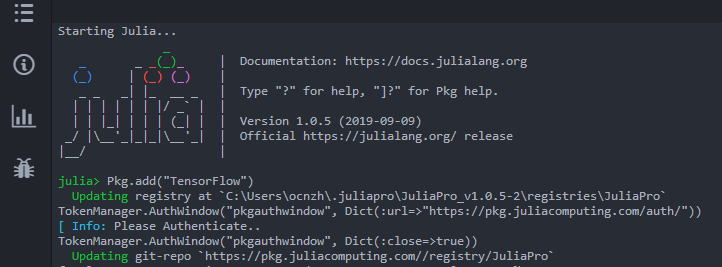
\includegraphics[width=0.86\textwidth]{Julia105de021001.PNG}
\caption{Julia V1.0.5}
\label{Julia105de021001}
\end{figure}
\begin{remark}
 过去动态语言大部分都是面向解释器设计, 这使得动态语言非常简单易学. 但实际上经常用程序不需要这么动态的特性, Julia平衡各种动态性, 去掉了一些不那么重要的动态性, 是面向JIT等优化技术设计的动态语言. Julia加入了一些限制, \href{https://www.zhihu.com/question/284356534/answer/437372256}{消除了Python和MATLAB的局限}.
 Julia可以调用大部分的R语言包. 虽然Julia学习曲线平滑, 但是想用Julia写出性能好, 抽象干净的代码是需要一定时间的.
 只有在科学计算这个领域, Julia目前才是更加合适的解决方案, 因为它为科学计算而生, 但是在其它领域Julia就几乎没有比较优势了.
 Python里使用Julia可以使用pyjulia.
 Julia可以调用MATLAB语言, 详情见包 \href{https://github.com/JuliaInterop/MATLAB.jl}{MATLAB.jl包}.
\end{remark}
%%%%%%%%%%%%%%%%%%%%%%%%%%%
\begin{figure}[H]
\centering
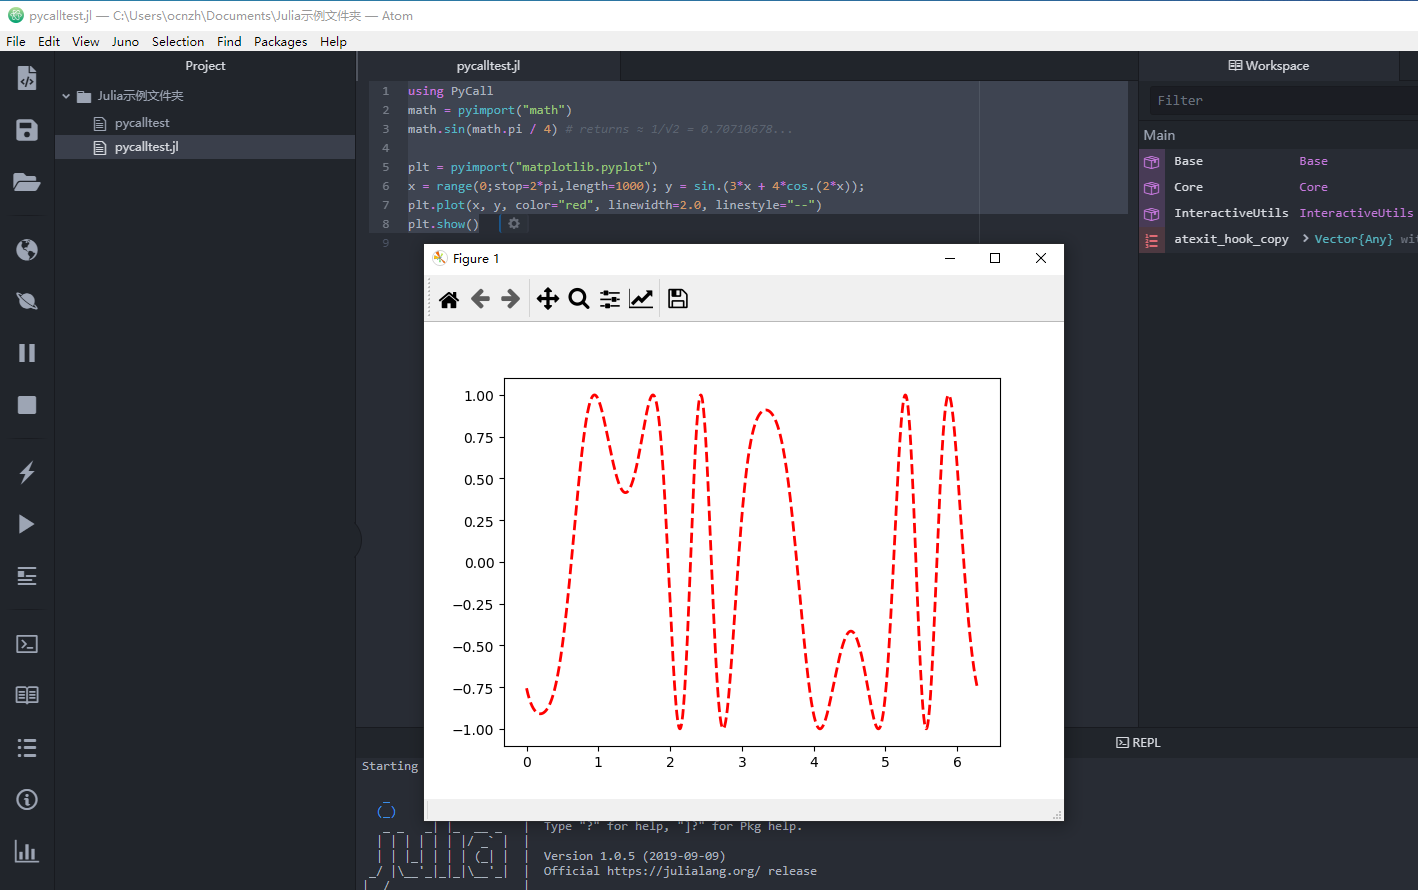
\includegraphics[width=0.7\textwidth]{Juliamatplotlib0211.png}
\caption{Julia使用Matplotlib}
\label{Juliamatplotlib0211}
\end{figure}
%%%%%%%%%%%%%%%%%%%%%%%%%%%
\begin{figure}[H]
\centering
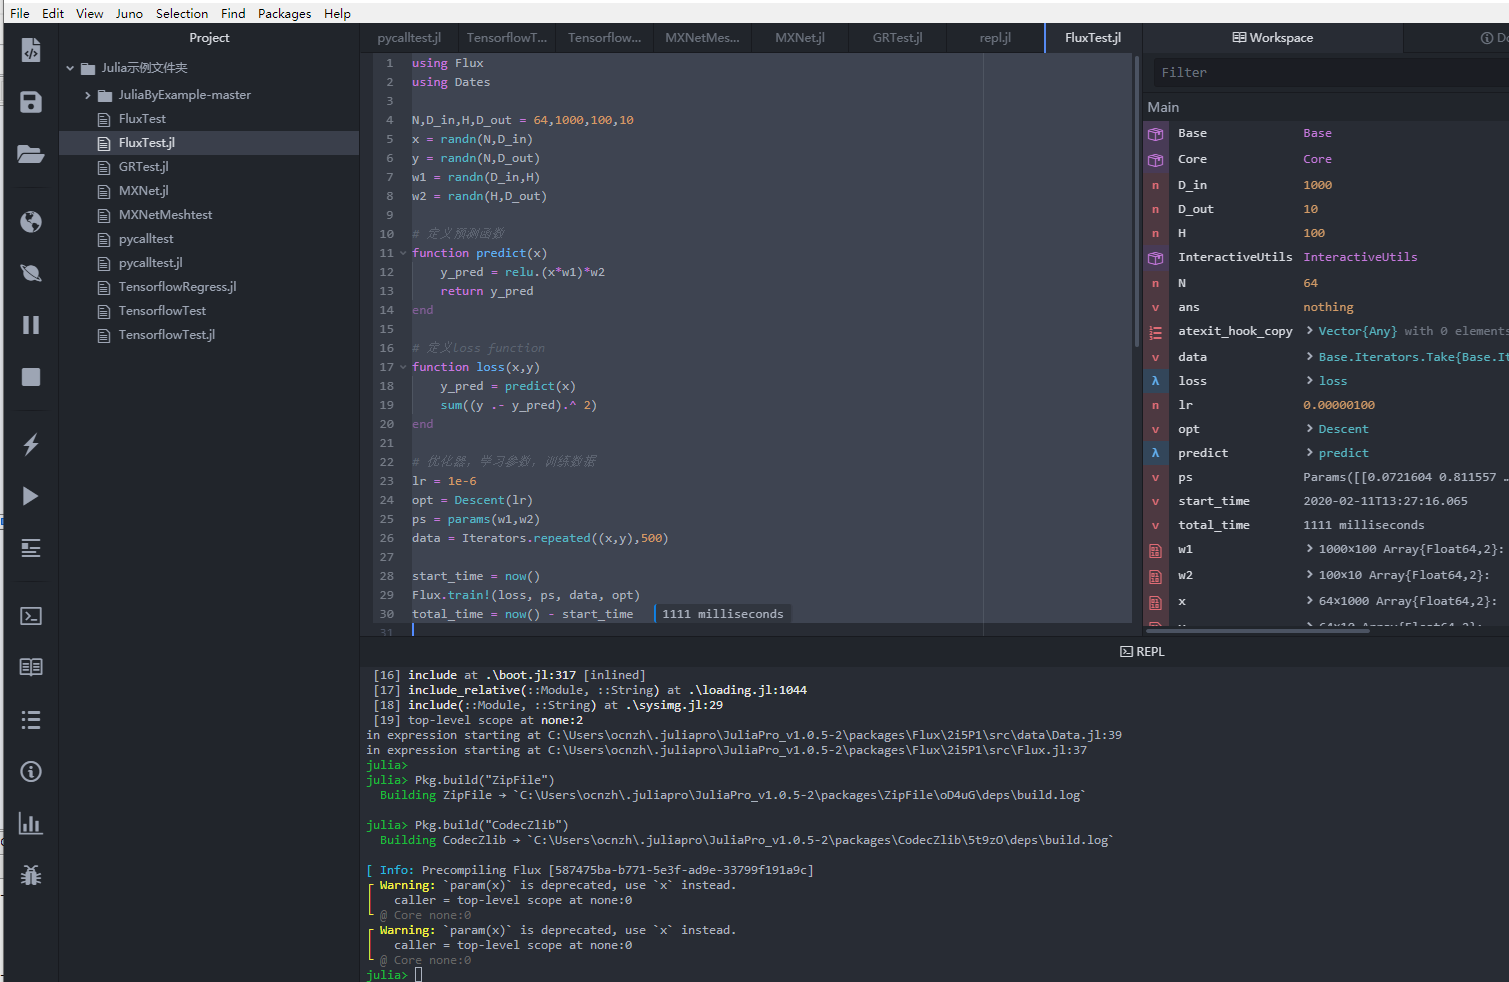
\includegraphics[width=0.7\textwidth]{JuliaFlux021101.PNG}
\caption{FLux宏包示例}
\label{JuliaFlux021101}
\end{figure}
%%%%%%%%%%%%%%%%%%%%%%%%%%%
\begin{figure}[H]
\centering
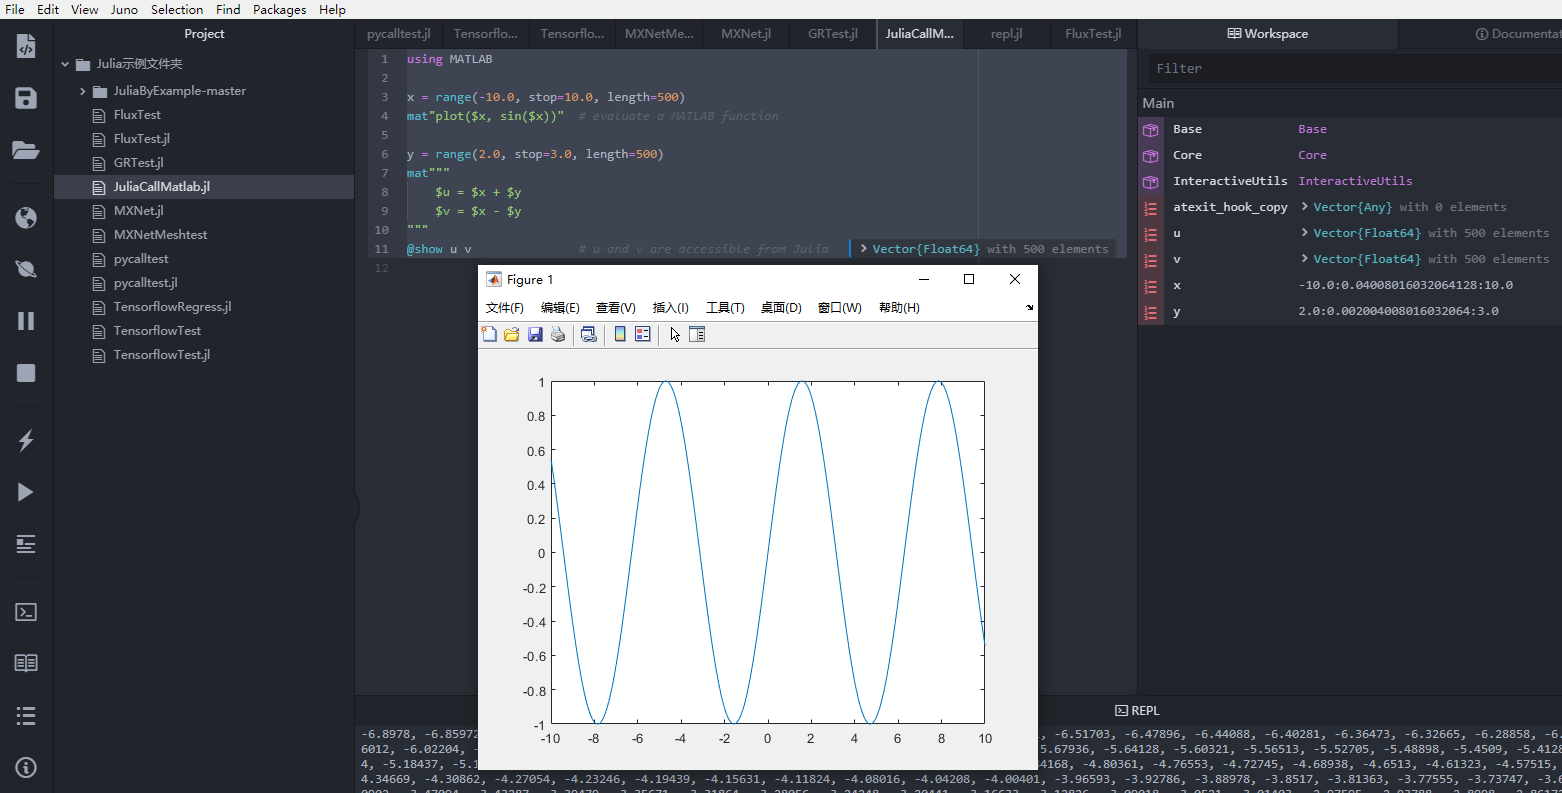
\includegraphics[width=0.7\textwidth]{JuliaMatlab021102.PNG}
\caption{调用MATLAB宏包}
\label{JuliaMatlab021102}
\end{figure}
自上世纪90年代以来, 编程语言Python已经取得了长足的进步.
Python含有优质的文档、丰富的AI库、机器学习库、自然语言和文本处理库. 尤其是Python中的机器学习, 实现了人工智能领域中大量的需求.
当Guido Van Rossum (1956年1月31日-)开发Python时, 他几乎不知道Python会成为世界上最流行的语言之一.
今天, Python是人类历史上使用最广泛的编程语言之一, 应用于很多程序中. 无论是企业级应用程序, 还是机器学习/人工智能模型、数据科学工作, Python几乎在所有蓬勃发展的行业和领域中都受人青睐.
全世界有超过800万的开发人员出于各种目的热衷于使用Python. 由于其\uwave{动态特性和易扩展性}, Python已经成为开发人员的首选语言. 这也是Python能够击败Java的原因,
而Java一度以来都是开发人员最喜欢的语言. 由于语言的自然老化, Java正在自然老去. 大多数新语言都是为解决现代面临的新挑战而设计的.
之前开发的语言在解决当时的问题时效率极高, 但要让它们跟上不断变化的行业和市场就变得极其困难.
但是, Python作为一种拥有如此庞大用户和开发者支持的开源语言, 即使在今天仍然保持着它的巅峰状态.
它丰富的库和内置的功能使其成为企业、开发人员和数据科学家的热门选择. 尽管Java仍然被用于企业开发, 但它在其他领域的相关性几乎为零.
很难发现一个机器学习专家在Java上设计和训练模型. 尽管如此, Java是全球第二大最受开发人员欢迎的语言.

Python已经成功地在大多数领域取代了Java. 在企业开发方面, Java面临着来自谷歌的新编程语言Go的威胁. 随着我们进入未来科技时代, 对高性能计算的需求也在不断增长. 这也是数据科学和人工智能的时代需求. 尽管有人可能认为使用extreme GPU有助于提高速度和效率, 但事实远非如此. 它不能满足特定的数据处理需求. 相反, 前沿应用程序需要其他依赖项来优化性能, 并帮助科学家和开发人员实现预期的目标. 最终, 这将引导企业和研究机构寻找更健壮的编程语言, 为特定的任务及其交付速度而设计.

在这个人人都喜爱Python的时代, 正面临着来自编程语言世界的新参与者——Julia的威胁. 这几年来我们能够感受到从MATLAB到Python的过渡. 我们知道机器学习几乎在所有应用程序中使用, 而且Python库使ML模型的实现更加容易, 所以人们转向了Python. 在此之前, MATLAB是这项任务的最佳选择, 可以帮助人们进行分析和科学计算. 但是很明显, 人们会把目光转向更容易实现、容易理解、更快速、更高性能和可扩展的解决方案. 因此, Python完美地填补了JAVA和MATLAB的空白.

3.8版的 Python语言引入一个独特的算子. 被称为海象算子(Walrus Operator)或命名表达式算子(Named Expression operator), 记为「:=」. 海象算子 这个新算子(:=)能让我们为表达式中的一个变量赋值, 看起来类似于海象的眼睛和犬齿.
%%%%%%%%%%%%%%%%%%%%%%%%%%%%%%%%%%%%
\begin{figure}[htbp]
\centering
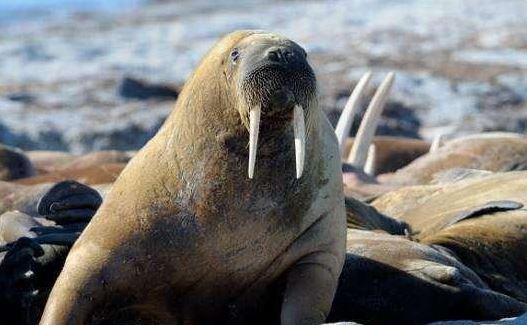
\includegraphics[width=0.65\textwidth]{Python20191228072329.jpg}
\caption{海象}
\label{Python2019122807232918}
\end{figure}
%%%%%%%%%%%%%%%%%%%%%%%%%%%%%%%%%%%%%%
\begin{example}
海象算子可以在 if 语句之中直接执行声明和赋值操作.
\begin{itemize}
\item ifcountry\_size:=len(countries)<5:print("Lengthofcountriesis"+country\_size)
\item employees=[resultforidinemployee\_idsif(result:=fetch\_employee(id))]
\item whilechunk:=file.read(256):process(chunk)
\end{itemize}
\end{example}

海象算子是作为 PEP-572(Python 改进提议)的一部分而引入的. 海象算子的争议点:
\begin{itemize}
\item 句法变化问题:开发者们为 := 提议了多种替代方案, 比如「表达式 -> NAME」、「NAME -> 表达式」、「{表达式} NAME」等等. 少数人建议使用现有的关键字, 其他人则使用了新的算子.
\item 后向兼容问题:这个特性无法向后兼容, 也无法运行在之前的 Python 版本上.
\item 算子名称问题:人们建议不要使用「海象算子」这样的代号, 而是使用「赋值算子」、「命名表达式算子」、「成为算子」等术语, 以免人们不明白.
\end{itemize}

Julia和Python之间的一个关键区别是处理特定问题的方式. Julia的构建是为了减轻高性能计算的挑战. 尽管Python现在已经发展为一种快速的计算语言, 但是我们必须承认它不是为这项工作而设计的. 然而, Julia是专门为高速处理和计算工作设计的. 虽然它只有几个月的历史, 却已经在研究人员和数据科学家中引起轰动.
两个月前, Julia发布了一个稳定的版本, 称为 \href{https://julialang.org/}{Julia 1.3}, 它已经得到了进一步的改进, 可以有效地处理大量占用资源的数据科学项目. 目前有超过800名Julia开发人员, 他们正在为GitHub做贡献, 帮助其成为首选语言.

Python 编辑器——Google Colaboratory

Colab 是一个免费的 Jupyter Notebook 环境(你可以想成是网页版多功能笔记本), 它不需要进行任何设置就可以使用, 并且完全在云端运行.

Tensorflow云端示例: \href{https://colab.research.google.com/drive/1bHPCray2HwwuFwpiA_KH6Klkc3aB_6oh}{Colab},
%%%%%%%%%%%%%%%%%%%%%%%%%%%%%%%%%%%%
\begin{figure}[htbp]
\centering
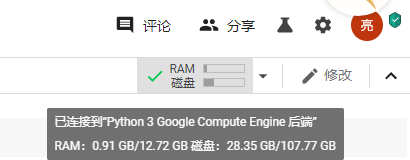
\includegraphics[width=0.65\textwidth]{GoogleComputeEngineColab1.PNG}
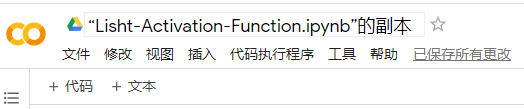
\includegraphics[width=0.65\textwidth]{GoogleComputeEngineColab2.PNG}
\caption{google-colab云端python编辑器}
\label{GoogleComputeEngineColab1}
\end{figure}

Anaconda 是一个基于 Python 的数据处理和科学计算平台, 它已经内置了许多非常有用的第三方库, 装上Anaconda, 就相当于把 Python 和一些如 Numpy、Pandas、Scrip、Matplotlib 等常用的库自动安装好了, 使得安装比常规 Python 安装要容易. 如果是学习Python的小白, 直接安装Anaconda+Pycharm就可以.
%%%%%%%%%%%%%%%%%%%%%%%%%%%%%%%%%%%%
\begin{figure}[htbp]
\centering
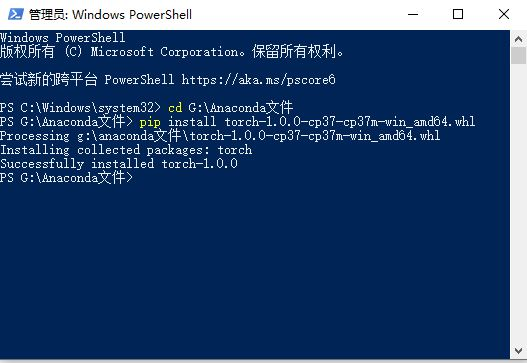
\includegraphics[width=0.65\textwidth]{pytorch20191218.JPG}
\caption{Cuda90-torch-1.0.0-cp37-cp37m-win\_amd64安装}
\label{pytorch20191218}
\end{figure}
%%%%%%%%%%%%%%%%%%%%%%%%%%%%%%%%%%%%
\begin{figure}[htbp]
\centering
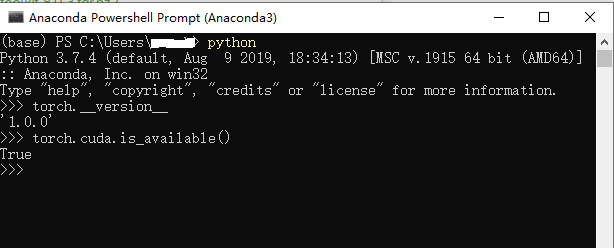
\includegraphics[width=0.65\textwidth]{Anaconda3torch1218.png}
\caption{Anaconda下测试torch包和Cuda90是否安装成功}
\label{Anaconda20191218}
\end{figure}

文件名列表
\begin{itemize}
\item \href{https://repo.anaconda.com/archive/Anaconda2-2019.10-Windows-x86\_64.exe}{Anaconda3-2019.10-py3.7Windows-x86\_64.exe}

\item \href{https://download.pytorch.org/whl/cu90/torch-1.0.0-cp37-cp37m-win\_amd64.whl}{torch-1.0.0-cp37-cp37m-win\_amd64.whl}, \href{https://pytorch.apachecn.org/docs/1.2/}{Pytorch 1.2帮助文档}

\item \href{https://pan.baidu.com/s/1EGRWJeW522xzPjCkF_Fzlw}{PyCharm Professional 2019.2.5},  提取码: m7d3, PyCharm Professional 2019.2.5的启动界面如图\ref{Pycharm20191218001}.
\end{itemize}
%%%%%%%%%%%%%%%%%%%%%%%%%%%%%%%%%%%%
\begin{figure}[htbp]
\centering
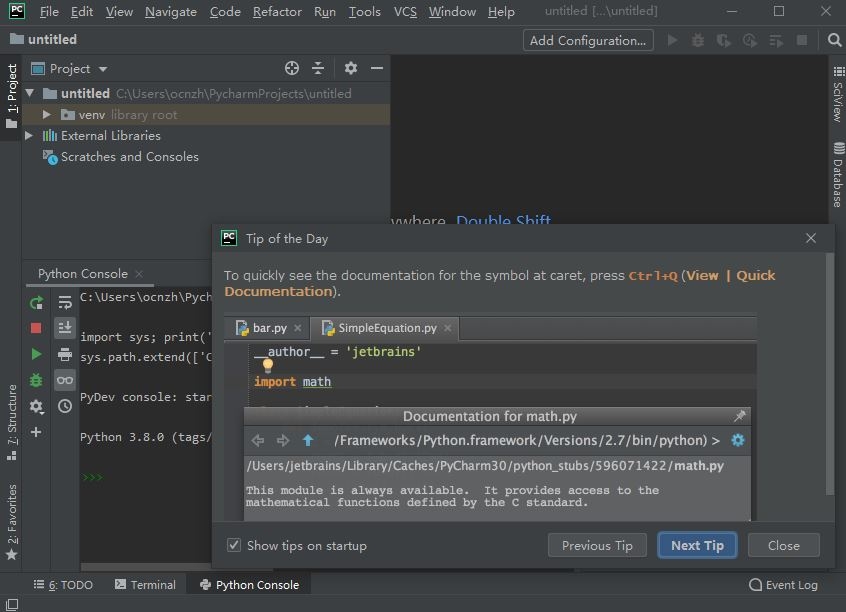
\includegraphics[width=0.65\textwidth]{Pycharm201925.JPG}
\caption{Pycharm 2019.2.5启动界面}
\label{Pycharm20191218001}
\end{figure}

创建项目并配置Anaconda, 首先点击create new project, location为文件存储位置, project interpreter为解释器, 也就是Anaconda中的python.exe, 按图\ref{PycharmAnacondaiter1218001}中步骤操作.
%%%%%%%%%%%%%%%%%%%%%%%%%%%%%%%%%%%%
\begin{figure}[htbp]
\centering
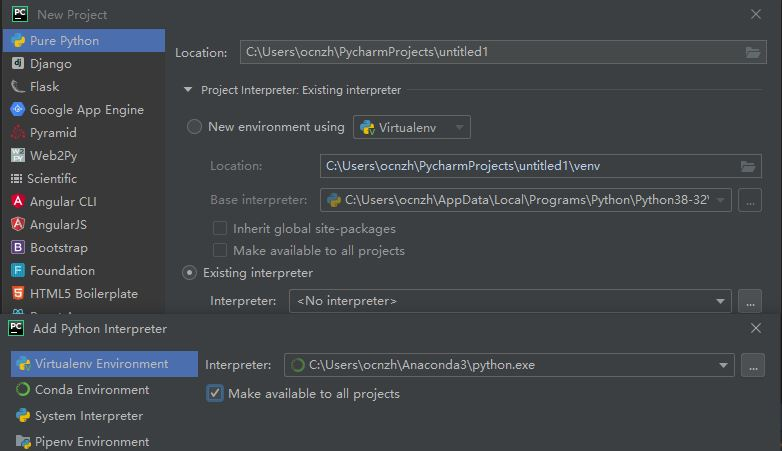
\includegraphics[width=0.65\textwidth]{PycharmAnacondaiter.JPG}
\caption{Pycharm中配置使用Anaconda中的python}
\label{PycharmAnacondaiter1218001}
\end{figure}
在file选项中选择default setting, 选择project interpreter并且按步骤选中Anaconda中的python.exe.
最后点击create(图\ref{PycharmAnacondaiter1218002}), 创建完之后进入pycharm界面, 点击close.
图\ref{PycharmPytorchDemo}是在ycharm中运行 two\_layer\_net\_tensor.py示例.
%%%%%%%%%%%%%%%%%%%%%%%%%%%%%%%%%%%%
\begin{figure}[H]
\centering
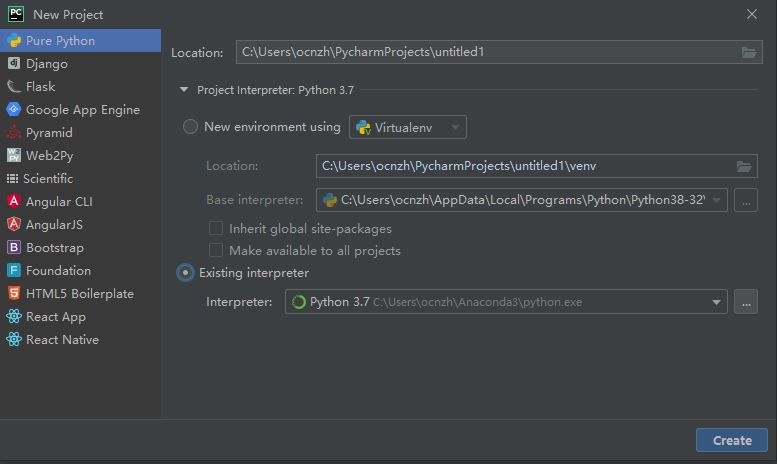
\includegraphics[width=0.65\textwidth]{PycharmAnacondaiterOk.JPG}
\caption{Pycharm中配置使用Anaconda中的python}
\label{PycharmAnacondaiter1218002}
\end{figure}
%%%%%%%%%%%%%%%%%%%%%%%%%%%%%%%%%%%%
\begin{figure}[htbp]
\centering
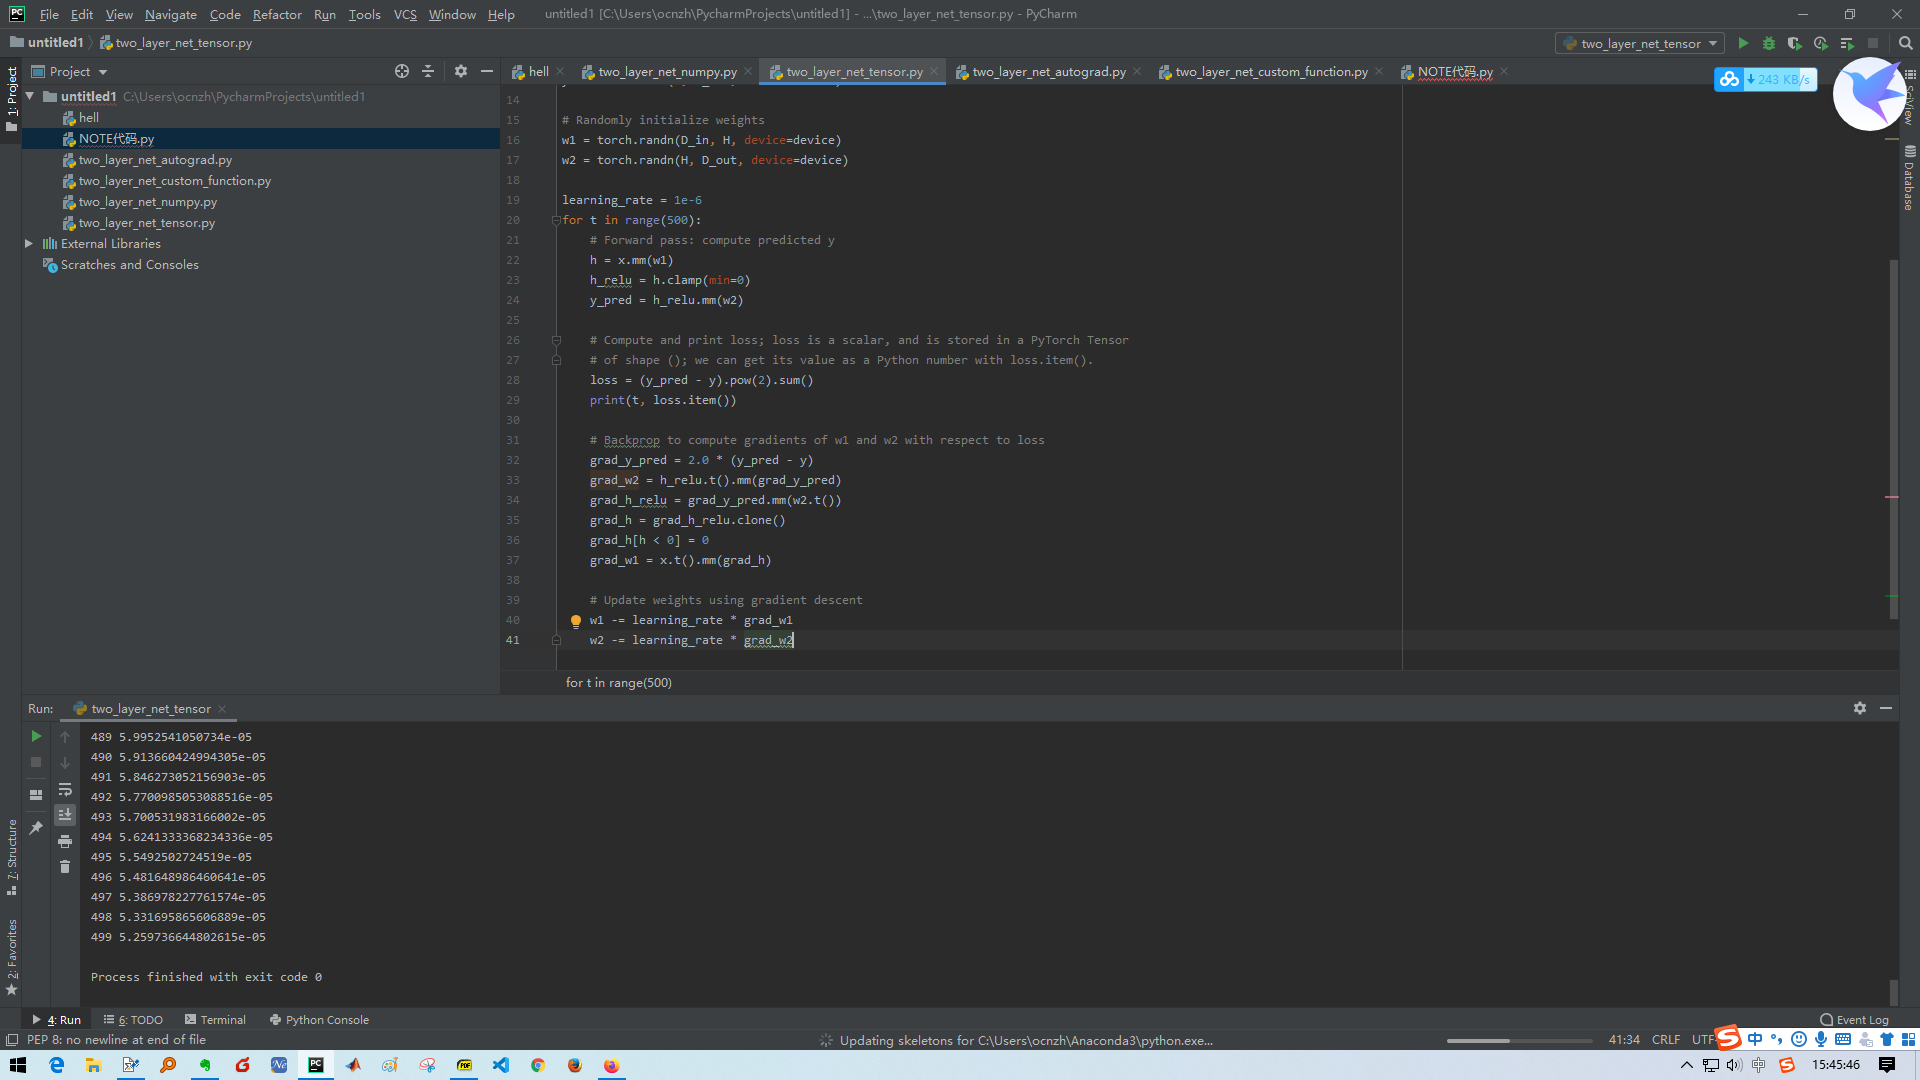
\includegraphics[width=0.85\textwidth]{PycharmPytorchDemo.png}
\caption{Pycharm中运行two\_layer\_net\_tensor.py}
\label{PycharmPytorchDemo}
\end{figure}

Python四个重要应用:验证算法、快速开发、测试运维、数据分析
\begin{itemize}
\item 验证算法:就是对我们公司常见设计算法或者公式的验证, 公式代码化.
\item 快速开发:就是用更少的代码来开发网站, Python在网站前后台有大量的成熟的框架, 如django, flask, bottle, tornado, flask和django的使用较多, 国内用Python开发的网站有:知乎、豆瓣、扇贝、腾讯、阿里巴巴;
\item 测试运维:用python实现的测试工具及过程, 包含服务器端、客户端、web、andriod、client端的自动化测试, 自动化性能测试的执行、监控和分析, 常用selenium appium等框架.
做运维同学应该清楚, 在Linux运维工作中日常操作涵盖了监控, 部署, 网络配置, 日志分析, 安全检测 等等许许多多的方面, 无所不包. python可以写很多的脚本, 把“操作”这个行为做到极致.
Python在服务器管理工具上非常丰富, 配置管理(saltstack) 批量执行( fabric, saltstack) 监控(Zenoss, nagios 插件) 虚拟化管理( python-libvirt) 进程管理 (supervisor) 云计算(openstack) ...... 还有大部分系统C库都有python绑定.
\item 数据分析:Python有三大神器:numpy,scipy,matplotlib,其中numpy很多底层使用C语言实现的, 所以速度很快, 用它参加各种数学建模大赛, 完全可以替代r语言和MATLAB.
\end{itemize}

%%%%%------------------------------------------------------------
\href{https://github.com/google/TensorNetwork}{Tensornetwork}

利用别的软件下的pip3文件安装tensornetwork, 假设如下路径
\begin{Verbatim}
    C:\Users\ocn***\Anaconda3\pkgs\pip-19.2.3-py37_0\Scripts

    D:\Program Files (x86)\Microsoft Visual Studio
      \Shared\Python37_64\Scripts
\end{Verbatim}
默认情况下, Windows PowerShell 不会从当前位置加载命令. 如果信任此命令, 切换到其中一个目录后, 键入“.$\backslash$pip3 install tensornetwork”

查看python安装位置

\quad python -version

\quad import sys

\quad sys.executable

所有python的路径: whereis python

当前使用的python路径: which python

升级pip: python -m pip install --upgrade pip
%%%%%%%%%%%%%%%%%%%%%%%%%%%%%%%%%%%%
\begin{figure}[htbp]
\centering
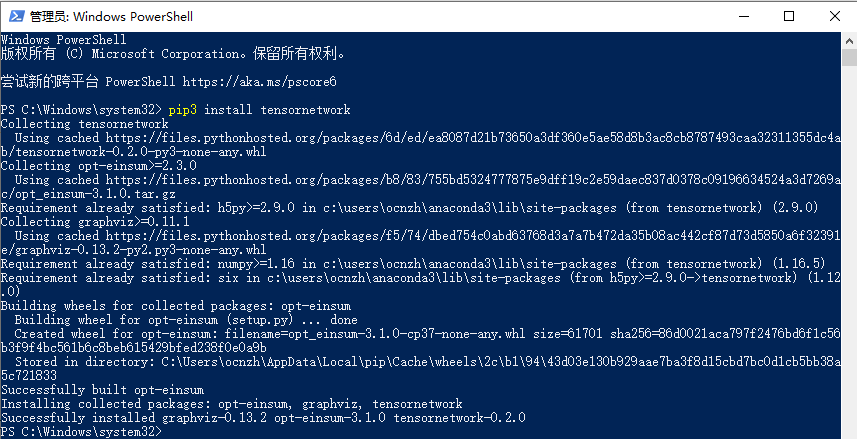
\includegraphics[width=0.85\textwidth]{Tensornetwork0118.PNG}
\caption{pip3文件安装tensornetwork}
\label{Tensornetwork0118}
\end{figure}

代码: TensorNN.py
\href{https://git-scm.com/download/win}{下载}
\includegraphics[width=0.05\textwidth]{gitlogo0130.png}

\href{https://morvanzhou.github.io/tutorials/machine-learning/theano/}{Theano的安装说明}
Theano是一个让你去定义, 优化, 计算数学表达式, 特别是多维数组(numpy.ndarray)的Python包. 具有速度快的特点, 支持GPU. Theano结合了计算机代数系统(computer algebra system, CAS)的特征和优化编译器的功能.
Theano 可以使用 GPU 进行运算, 用GPU运行比CPU快100倍左右, theano 是比较优秀的 python 模块.
theano.function可以被视为一个从纯符号图构建可调用对象的编译器接口, 重要的特征之一是theano.function能够优化图, 甚至能够将图的一部分或者全部编译成简单的机器指令.
%%%%%%%%%%%%%%%%%%%%%%%%%%%%%%%%%%%%
\begin{figure}[htbp]
\centering
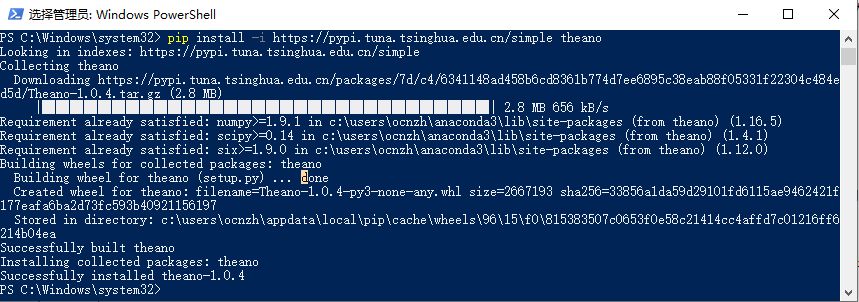
\includegraphics[width=0.85\textwidth]{theano2020020701.PNG}
\caption{安装theano}
\label{theano2020020701}
\end{figure}

\href{http://rll.berkeley.edu/cgt/}{CGT}
%%%%%%%%%%%%%%%%%%%%%%%%%%%%%%%%%%%%
\section{AI研究的基本内容}
现在, 人类社会正在进入第四次技术革命, 就是以互联网、大数据和人工智能技术驱动的技术革命, 它会推动人类社会生活生产方式进入自动化时代, 人工智能时代. 而人类社会的教育, 特别是学校教育, 将会发生什么样的变化?具体来说有以下几个领域.

\textcolor[rgb]{0,0,1}{一}、\Circled{教育的人文性}. 也就是教育的价值转型, 人文是教育的本质. 脑科学证明, 在人类接受幼儿和学校教育的阶段, 离不开师生交往和生生交往. 从这个意义上来看, 教师不会被技术取代, 需要转型的是教育的价值导向. 我认为, 技术变革使未来匮乏的不再是征服世界和改造世界的能力, 而是对于人的心理、情感和品德的培养.

\textcolor[rgb]{0,0,1}{二}、\Circled{教育的全域化特点}. 在技术革命的影响下, 学校教育、家庭教育和社会教育的边界正在解构. 在全域教育时代, 如何使学校教育线上线下融合、学校家庭沟通协同、校内和校外衔接、学校和社区共治, 这是未来教育重大的挑战.

\textcolor[rgb]{0,0,1}{三}、\Circled{教育的集智性}. 教育将从过去封闭的、个体化的教学, 转向开放的集智化教学时代. 随着人工智能的发展, 教育合作将基于人力配置进行重组, 家庭与学校的教学协同性, 教育资源配置的协同性都将产生重大变化.

\textcolor[rgb]{0,0,1}{四}、\Circled{教育的自组织性}. 未来教育将从过去的班级授课制转变为学习共同体, 学校的功能定位要从过去服务于知识传承的教学型组织, 转向服务自主探究的学习型组织. 面向未来, 应该推进学习型组织的转变, 把传统教室进行改造, 开展社团学习活动以及鼓励教师进行自组织教学活动.

\textcolor[rgb]{0,0,1}{五}、\Circled{教育的个体性}. 传统教育是同质化的, 是按照统一的课程标准、教材、班级, 以及统一的备课、上课、考试评价进行的. 而未来强调人的主体性、个性化、差别化, 我们要从知识的教学转向核心素养的教育. 必须要改变传统的教学方式, 也就是课程的供给方式要去同质化, 要把统一的知识教学和针对个人的定制
教育结合并存.

\textcolor[rgb]{0,0,1}{六}、\Circled{教育的综合化}. 未来课程组织的逻辑将从分科走向综合, 传统的课程体系学科彼此独立. 而今天的教育变革强调跨学科、主题性, 要将课程去学科化, 增加主题化、跨学科和生活化的教育, 也就是将学科课程逻辑与实践课程逻辑相结合.
此外, 教育还要为学生提供试错的机会和发展潜能的平台, 要注重学生身心合一引导其进行自主建构的学习, 要将智能数据作为工具分析学生的学习状态、兴趣和优势, 以及未来教育还要开展多元合作治理等等.
(北京师范大学教授 |中国教育学会副会长 张志勇, 现代教育报, 2019-12-25)
%%%%%%%%%%%%%%%%%%%%%%%%%%%%%%%%%%%%
\subsection{AI 的 学 科 位 置}
AI是一门新兴的边缘学科, 是自然科学与社会科学的交叉学科
AI的交叉包括: 逻辑、思维、生理、心理、计算机、电子、语言、自动化、光、声等
AI的核心是思维与智能, 构成了自己独特的学科体系
AI的基础学科包括: 数学(离散、模糊)、思维科学(认知心理、逻辑思维学、形象思维学)和计算机(硬件、软件)等.

人工智能是最宽泛的概念, 机器学习则是实现人工智能的一种方式, 也是目前较有效的方式. 深度学习是机器学习算法中最热的一个分支, 在近些年取得了显著的进展, 并代替了多数传统机器学习算法. 所以, 三者的关系可用下图表示, 人工智能 > 机器学习 > 深度学习.
\begin{figure}[htbp]
	\centering
	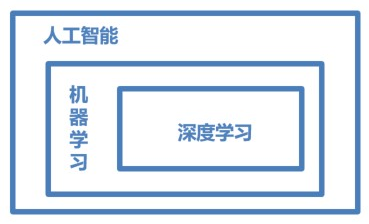
\includegraphics[width=0.5\textwidth]{AI2020012901.PNG}
	\caption{人工智能、机器学习和深度学习三者的关系}
   \label{AI2020012901}
\end{figure}
\begin{figure}[htbp]
	\centering
	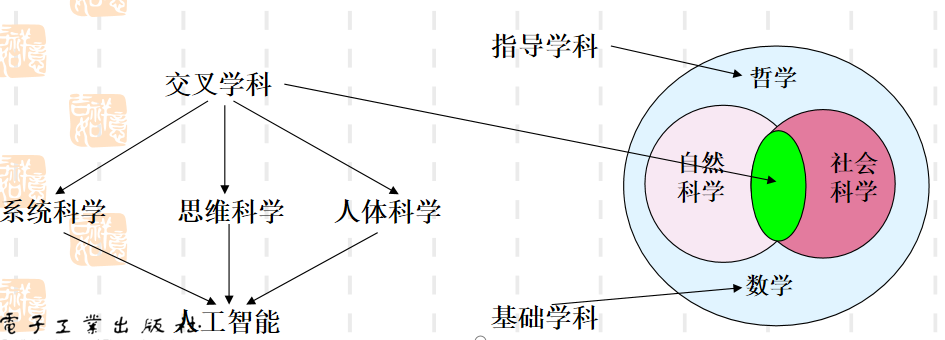
\includegraphics[width=0.5\textwidth]{Xuekeweizhi.png}
	\caption{学科树状示意图}
   \label{AI:XuekeweizhiFig2}
\end{figure}
%%%%%%%%%%%%%%%%%%%%%%%%%%%%%%%%%%%%%%%%%%
\begin{figure}[H]
\centering
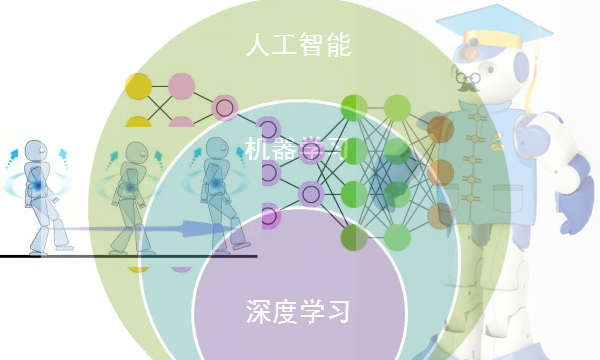
\includegraphics[width=0.5\textwidth]{MLDNN121801.png}
\label{MLDNN12019121501}
\end{figure}
AI的研究方向分为2个层次,第1层分为计划于调度、专家系统、机器学习、推荐系统等。而机器学习还可以继续往下分,例如,有监督学习、无监督学习、深度学习等。在这2层分类中,发现了前面提到的机器学习和深度学习。
%%%%%%%%%%%%%%%%%%%%%%%%%%%%%%%%%%%%%%%%%%
\begin{figure}[H]
\centering
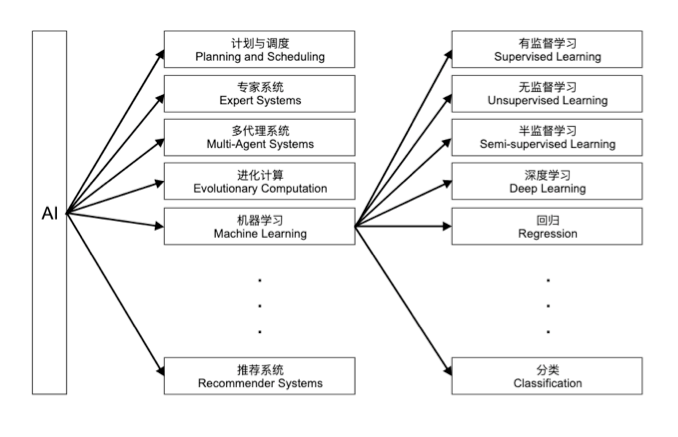
\includegraphics[width=0.38\textwidth]{AIstruc20200318133603.png}
\caption{AI研究的方向}
\label{AIstruc20200318133603}
\end{figure}
%%%%%%%%%%%%%%%%%%%%%%%%%%%%%%%%%%%%
\subsection{人工智能学科(F06)代码}
2020年度人工智能学科(F06)代码进行了较大调整, 大部分代码对应的内容都发生了变化, 比如增加了新的申请方向“F0602复杂性科学与人工智能理论”,
原申请方向“机器感知与模式识别”分拆为“F0604机器感知与机器视觉”和“F0605模式识别与数据挖掘”等.
%%%%%%%%%%%%%%%%%%%%%%%%%%%%%%%%%%%%
\subsection{与脑科学和认知科学的交叉研究-脑科学}
%%%%%%%%%%%%%%%%%%%%%%%%%%%%%%%%%
\begin{mydef}{脑科学}{1}
又称神经科学, 其目的是要认识脑、保护脑和创造脑. 美国神经科学学会的定义: 神经科学是为了了解神经系统内分子水平、细胞水平及细胞间的变化过程, 以及这些过程在中枢的功能、控制系统内的整合作用所进行的研究.
\end{mydef}
%%%%%%%%%%%%%%%%%%%%%%%%%%%%%%%%%
\begin{mydef}{脑的涵义}{1}
从狭义和广义两个方面来理解: 从狭义方面, 脑是指中枢神经系统, 有时特指大脑; 从广义方面, 脑可泛指整个神经系统. 人工智能是从广义角度来理解脑科学的, 因此它涵盖了所有与认识脑和神经系统有关的研究.
    人脑是自然界中最复杂、最高级的智能系统: 这种复杂性主要表现在人脑是由巨量神经元经其突触的广泛并行互联所形成的一个巨复杂系统.
\end{mydef}

现代脑科学的基本问题主要包括:

  (1) 揭示神经元之间的连接形式, 奠定行为的脑机制的结构基础;

  (2) 阐明神经活动的基本过程, 说明在分子、细胞到行为等不同层次上神经信号的产生、传递、调制等基本过程;

  (3) 鉴别神经元的特殊细胞生物学特性;

  (4) 认识实现各种功能的神经回路基础;

  (5) 解释脑的高级功能机制等.

脑科学是人工智能的基础: 研究的任何进展, 都将会对人工智能的研究起到积极的推动作用, 因此人工智能应该加强与脑科学的交叉研究, 以及人类智能与机器智能的集成研究.
%%%%%%%%%%%%%%%%%%%%%%%%%%%%%%%%%
\begin{mydef}{认知}{1}
认为是和情感、动机、意志相对应的理智或认识过程, 或者是为了一定的目的, 在一定的心理结构中进行的信息加工过程.
\end{mydef}

美国心理学家浩斯顿(Houston)等人把认知归纳为以下5种主要类型:

(1) 认知是信息的处理过程;

(2) 认知是心理上的符号运算;

(3) 认知是问题求解;

(4) 认知是思维;

(5) 认知是一组相关的活动, 如知觉、记忆、思维、判断、推理、问题求解、学习、想象、概念形成及语言使用等.

%%%%%%%%%%%%%%%%%%%%%%%%%%%%%%%%%
\begin{mydef}{认知科学}{1}
认知科学(亦称思维科学)是研究人类感知和思维信息处理过程的一门学科, 其主要研究目的就是要说明和解释人类在完成认知活动时是如何进行信息加工的.
\end{mydef}

认知科学也是人工智能的重要理论基础, 对人工智能发展起着根本性的作用. 认知科学涉及的问题非常广泛, 除了像浩斯顿提出的知觉、语言、学习、记忆、思维、问题求解、创造、注意、想象等相关联活动外, 还会受到环境、社会、文化背景等方面的影响.

从认知观点看, AI应同时开展对逻辑思维、形象思维和灵感思维的研究.


%%%%%%%%%%%%%%%%%%%%%%%%%%%%%%%%%%%%
\subsection{智能模拟的方法和技术研究}
\begin{itemize}
\item 机器感知: 就是要让计算机具有类似于人的感知能力, 如视觉、听觉、触觉、嗅觉、味觉.
      \begin{itemize}
         \item 机器视觉(或叫计算机视觉): 就是给计算机配上能看的视觉器官, 如摄像机等, 使它可以识别并理解文字、图像、景物等.
         \item 机器听觉(或叫计算机听觉): 就是给计算配上能听的听觉器官, 如话筒等, 使计算机能够识别并理解语言、声音等.
         \item 机器感知相当于智能系统的输入部分.
         \item 机器感知的专门的研究领域: 计算机视觉、模式识别、自然语言理解.
      \end{itemize}
\item 机器思维: 让计算机能够对感知到的外界信息和自己产生的内部信息进行思维性加工.
      \begin{itemize}
         \item 逻辑思维
         \item 形象思维
         \item 灵感思维
      \end{itemize}
\item 机器学习: 让计算机能够像人那样自动地获取新知识, 并在实践中不断地完善自我和增强能力.
      \begin{itemize}
         \item 机器学习方法: 机械学习、类比学习、归纳学习、发现学习、遗传学习和连接学习等.
      \end{itemize}
\item 机器行为: 让计算机能够具有像人那样地行动和表达能力, 如走、跑、拿、说、唱、写画等.  相当于智能系统的输出部分.
\item 智能系统与智能机器
      \begin{itemize}
         \item 无论是人工智能的近期目标还是远期目标, 都需要建立智能系统或构造智能机器.
         \item 需要开展对系统模型、构造技术、构造工具及语言环境等研究.
      \end{itemize}
\end{itemize}
%%%%%%%%%%%%%%%%%%%%%%%%%%%%%%%%%%%%
\section{AI研究中的不同学派——不同学派}
\begin{itemize}
\item 符号主义学派(逻辑主义和心理学派)
     \begin{itemize}
       \item 主要观点: AI起源于数理逻辑, 人类认知的基元是符号, 认知过程是符号表示上的一种运算.
       \item 代表性成果: 厄尔和西蒙等人研制的称为逻辑理论机的数学定理证明程序LT.
       \item 代表人物: 纽厄尔、肖、西蒙和尼尔逊(Nilsson)等.
    \end{itemize}
\item 连接主义学派(仿生学派或心理学派)
     \begin{itemize}
       \item 主要观点: AI起源于仿生学, 特别是人脑模型, 人类认知的基元是神经元, 认知过程是神经元的连接活动过程.
      \item 代表性成果: 由麦克洛奇和皮兹创立的脑模型, 即MP模型.
      \item 代表人物: 麦克洛奇和皮兹.
    \end{itemize}
\item 行为主义学派(进化主义、控制论学派)
     \begin{itemize}
        \item 主要观点: AI起源于控制论, 智能取决于感知和行为, 取决于对外界复杂环境的适应, 而不是推理.
        \item 代表性成果: 澳大利亚科学院院士、机器人专家Rodney Brooks教授研制的机器虫,  头衔: 澳洲科学院fellow、美国国家工程院院士、国际人工智能协会(AAAI)创始会员、作家、机器人企业家、MIT机器人教授、MIT计算机科学和人工智能实验室前主任、iRobot创始人及前CTO、RethinkRobotics前CTO及联合创始人.
        \item 代表人物:  Brooks教授,  是机器人行为主义学派的旗帜性人物. 而这位大神不仅在学术领域建树卓著, 在1997年上映的电影《又快又贱又失控》(Fast,  Cheap&Out of Control),  图\ref{AI:fyqincu540Fig2}.
    \end{itemize}
\begin{figure}[htbp]
	\centering
	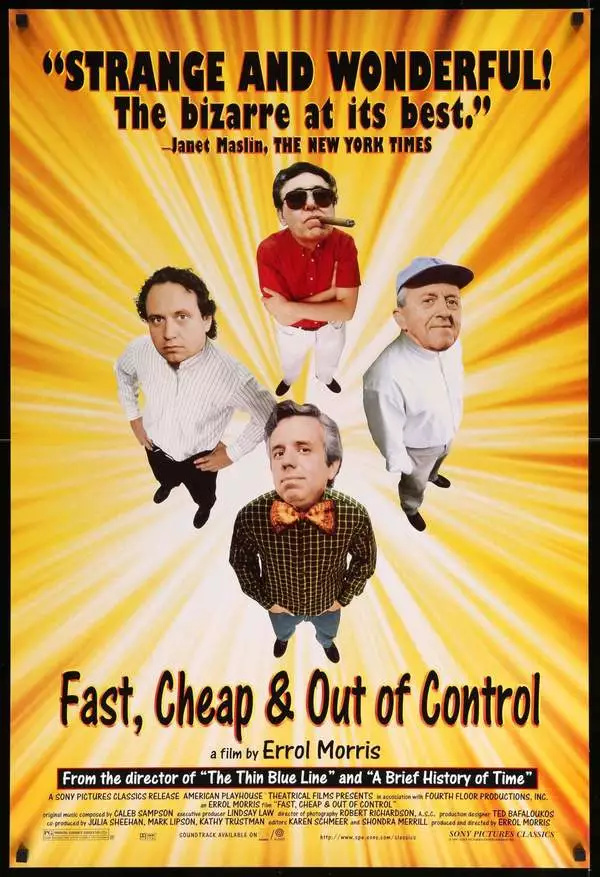
\includegraphics[width=0.4\textwidth]{9PWh-fyqincu5408120.jpg}
	\caption{电影《又快又贱又失控》}
   \label{AI:fyqincu540Fig2}
\end{figure}

\end{itemize}
%%%%%%%%%%%%%%%%%%%%%%%%%%%%%%%%%%%%
\paragraph{不同学派的理论之争}
\begin{itemize}
\item \textcolor{blue}{符号主义}

      智能的基础是知识, 其核心是知识表示和知识推理; 知识可用符号表示, 也可用符号进行推理, 因而可以建立基于知识的人类智能和机器智能的统一的理论体系.
\item \textcolor{blue}{连接主义}

      思维的基元是神经元, 而不是符号; 思维过程是神经元的联结活动过程, 而不是符号运算过程; 反对符号主义关于物理符号系统的假设.
\item \textcolor{blue}{行为主义}

      智能取决于感知和行动, 提出了智能行为的“感知—动作”模型; 智能不需要知识、不需要表示、不需要推理; 人工智能可以像人类智能那样逐步进化.

\item \textcolor{blue}{符号主义、功能模拟}

      构造能够模拟大脑功能的智能系统. 相当于“鸟飞”.
\item \textcolor{blue}{连接主义、结构模拟}

      构造模拟大脑结构的神经网络系统. 相当于“飞鸟”.
\item \textcolor{blue}{行为主义、行为模拟}

      构造具有进化能力的智能系统. 相当于“由猿到人”.
\end{itemize}
%%%%%%%%%%%%%%%%%%%%%%%%%%%%%%%%%%%%%%%%%%%
\begin{example}(全息AI)
微美全息WIMI专注于计算机视觉全息云服务. 据介绍, 微美全息覆盖从全息计算机视觉AI合成、全息视觉呈现、全息互动软件开发、全息AR线上及线下广告投放、全息ARSDK支付、5G全息通讯软件开发、全息人脸识别开发、全息AI换脸开发等全息AR技术的多个环节, 是一家全息云综合技术方案提供商. 其商业应用场景主要聚集在家用娱乐、光场影院、演艺系统、商业发布系统及广告展示系统等五大专业领域.
\end{example}
%%%%%%%%%%%%%%%%%%%%%%%%%%%%%%%%%%%%
\section{人工智能近期发展分析}
人工智能自提出到现在已与经历60多年的演化和发展, 在移动互联网、大数据、超算、传感网络、脑科学等理论和技术驱动以及经济社会发展需求牵引下, 呈现出强劲和加速发展的势头;
以强化学习、深度学习及宽度学习等为代表的先进学习方法得到了迅猛发展, 在解决大数据驱动知识学习、跨媒体协同处理、人机物协同增强智能、群体集成智能、自主智能系统等领域关键技术问题中发挥了非常关键性的作用;
与此同时, 类脑智能的研究与开发工作也同样受到国内外相关研究机构和学者的高度关注及重视, 为人工智能的深入快速发展迎来了机遇和挑战.

人工智能已经走过50多年的历史, 下一步该如何发展, 是人工智能学者最为关心的一个问题. 但要准确回答这一问题却又十分困难, 下面所给出的分析(6个方面)仅是对国内外学者的一些观点的归纳.
%%%%%%%%%%%%%%%%%%%%%%%%%%%%%%%%%%%%
\subsection{人工智能发展方向}
\subsubsection{人工智能应用前景}
\begin{figure}[H]
\centering
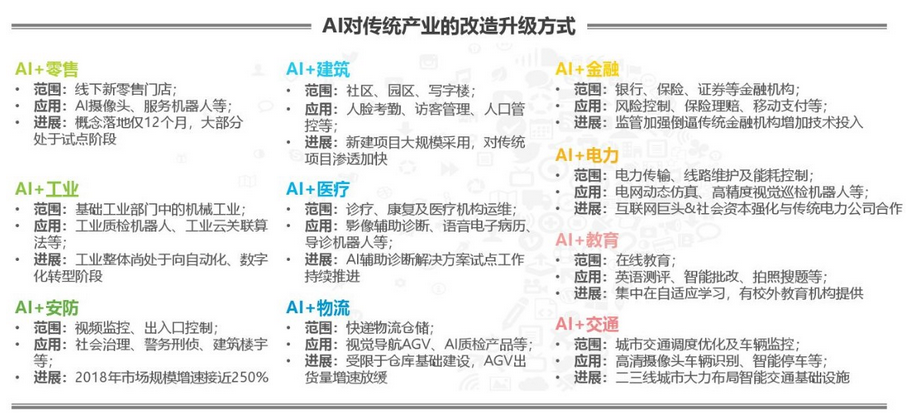
\includegraphics[width=0.86\textwidth]{AIqushi013002.PNG}
\caption{以深度学习为基础的AI技术的应用}
\label{AIqushi013002}
\end{figure}
%%%%%%%%%%%%%%%%%%%%%%%%%%%%%%%%%%
\subsubsection{人工智能近期发展方向}
人工智能的产业化前景(人机物三元协同控制与决策优化的角度):人机物智能技术就是综合应用物联网、移动互联网、通信、大数据计算、人工智能等技术使物与物之间、人与物之间实现互联和互通, 并通过协同仿真、分布计算、跨平台管控等智能处理技术实现人与万物的协同工作. 利用人机物三元协同的智能技术, 使人类社会、虚拟空间、自然空间、机器物理空间实现联通互动、数字双生、虚实交融, 形成以人为中心人机物三元融合的协同工作场景. 人机物共融将推进生产方式向智能技术领域演化, 同时也体现了智能制造的标志性特征. 将人的联想、推理、反馈、学习、理解等能力与机器的搜索、作业、推理、学习等能力相融合, 解决人机物三元分布式协同控制与决策优化问题. 在复杂制造系统的生产计划、质量管控、设备维护和制造执行等企业的各个应用管理层面均体现了人机物三元协同与融合技术的普适性.
%%%%%%%%%%%%%%%%%%%%%%%%%%%%%%%%%%%%
\paragraph{多学科交叉研究}

人工智能理论基础研究强调与脑科学、认知科学、心理学、信息科学、生物学、逻辑学、物理学和数学等学科的交叉研究.
\begin{itemize}
\item  脑科学为人工智能研究提供人脑神经系统功能的本质和机理;
\item  认知科学为人工智能研究提供感知、思维、学习和语言等基本原理;
\item  心理学为人工智能研究提供认知、情感、意识等心理过程及联系;
\item  生物学为人工智能研究提供自然界生物运行的机制;
\item  逻辑学为人工智能研究提供思维规律描述的理论和方法;
\item  信息科学为人工智能研究提供模拟的物质基础和技术手段;
\item  数学为人工智能研究提供各种有效的计算模型和方法.
\end{itemize}
%%%%%%%%%%%%%%%%%%%%%%%%%%%%%%%%%%%%
\paragraph{集成智能研究}

智能的物质、能量、信息基础: 自然智能是一种基于“碳”的信息处理, 人工智能是一种基于“硅”的信息处理, 尽管这两种信息处理所基于的物质不同, 但它们的运算能量的都应该是电信号. 那么, 是否可以在“碳”和“硅”这两种不同物质上建立一种基于电信号的统一的信息处理模型?
\begin{Verbatim}
    人类的智能: 物质(碳)+能量(生物电)→ (生物)信息.
    人造的智能: 物质(硅)+能量(物理电)→ (电子)信息.
    集成智能的研究: 脑-机接口(Brain-Computer Interface, BCI)的研究成果.
          进一步证实了集成智能的可能性和辉煌前景.
\end{Verbatim}
智能产生机理测试, 图\ref{AItest2020012801}.
%%%%%%%%%%%%%%%%%%%%%%%%%%%%%%%
\begin{figure}[htbp]
\begin{center}
\begin{tikzpicture}[font={\sf \small}]
\def \shiftx{2cm}
%\node[judge,good,minimum size=1cm] at (0,0){主持人};
%\node[sailor,good,minimum size=1cm] at (2,0){普通的被测试者};
%\node[conductor,female,good,minimum size=1cm] at (-2,0){};
\node[name=a,shape=maninblack,monitor,saturated,minimum size=1cm,yshift=-4.05cm] {主持人};
\node[name=b,shape=graduate,monitor,saturated,minimum size=1cm,xshift=-3.25cm] {普通的被测试者};
\node[name=c,shape=graduate,monitor,saturated,minimum size=1cm,mirrored,xshift=3.25cm] {含脑芯片的被测试者};
\draw[thick,blue,->] (a.south) parabola (c.south);
\draw[thick,blue,->] (a.south) parabola (b.south);
\node[ellipse callout, draw,yshift=-0.28cm, callout absolute pointer={(a.mouth)}] {小于50\%吗?};
%\node[ellipse callout, draw, yshift=-.3cm, callout absolute pointer={(b.mouth)},font=\tiny] {普通的被测试者};
%\node[ellipse callout, draw, yshift=-.3cm, callout absolute pointer={(c.mouth)},font=\tiny] {含脑芯片的被测试者};
\end{tikzpicture}
\end{center}
\caption{智能产生机理测试}
\label{AItest2020012801}
\end{figure}
%%%%%%%%%%%%%%%%%%%%%%%%%%%%%%%%%%%%
\paragraph{多学派融合研究}

融合是一种必然趋势: 符号主义、联结主义和行为主义三大学派各有所长、各有所短, 它们各自经过一段时间的分立研究之后, 正逐步开始走向融合. 多学派融合是人工智能发展的一种必然趋势.

融合需要解决的关键问题:

(1) 不同学派之间的共同机制是什么?

(2) 怎样建立一个统一的智能理论体系?

(3) 如何真正实现它们之间的有机融合等.
%%%%%%%%%%%%%%%%%%%%%%%%%%%%%%%%%%%%
\paragraph{智能网格}

互联网是人类历史上发展速度最快的一次技术革命, 但目前仍处于发展的初级阶段, 其智能水平还很低.
未来的互联网应该是一种具有自动调整功能, 各个节点之间协调工作, 能为用户提供便利、有效服务的智能网络.
%%%%%%%%%%%%%%%%%%%%%%%%%%%%%%%%%%%%
\paragraph{智能机器人研究}

智能机器人将会对社会生产力发展和人类社会进步, 以及对人们生活、工作和思维方式的改进等产生不可估量的影响(例如, 海军总医院的手术机器人“黎元”, 可通过互联网完成远程颅脑手术).
未来智能机器人应该是一种具有人类感知、行为能力, 超强记忆、学习、推理、规划能力, 有情感、人性化, 能代替人类在真实环境中自主工作的机器人.
%%%%%%%%%%%%%%%%%%%%%%%%%%%%%%%%%%%%
\paragraph{智能应用和智能产业}

智能技术将进一步与主流信息技术融合, 并将应用于人类社会的各个领域和人类生活的各个方面.
有人预计: 智能产业将逐步成为社会第四产业; 智件将逐步从软件中分离出来, 成为智能计算机系统的三件(硬件、软件、智件)之一.

《机器人和人工智能的崛起》一书的作者Martin Ford说:“机器人崛起的可能性很大, 自动化在最初的不稳定性对发展中国家的影响更大, 而最终的结果则取决于我们如何选择、我们如何作为以及我们如何适应这种状况. ”
%%%%%%%%%%%%%%%%%%%%%%%%%%%%%%%%%%%%
\subsection{人工智能发展八大新趋势}
人工智能(AI)是物联网及工业4.0发展的核心. 尤其, 当特斯拉(Tesla)推出电动车及苹果(Apple)推出FaceID之后, 让市场体验到AI芯片的无限商机. 同时, AI应用接受度越高的国家, 将对其GDP产生贡献愈大.
%%%%%%%%%%%%%%%%%%%%%%%%%%%%%%
\begin{figure}[htbp]
	\centering
	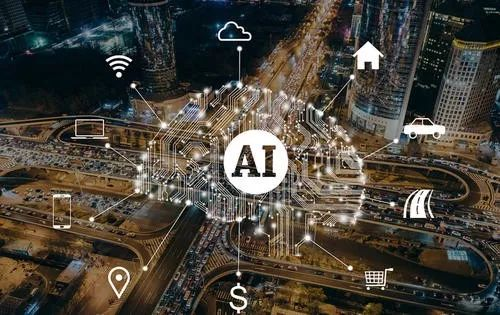
\includegraphics[width=0.5\textwidth]{AI20191218182232.jpg}
	\caption{示意图}
   \label{AI20191218182232Fig4}
\end{figure}
AI芯片包含三大类市场, 分别是数据中心(云端)、通信终端产品(手机)、特定应用产品(自驾车、头戴式AR/VR、无人机、机器人...). 当前机器学习多采用GPU图像处理, 尤以Nvidia是此一领域龙头, 但是, 有些业者认为GPU处理效率不够快, 而且因应众多特定新产品的不同需求, 于是, 推出NPU、VPU、TPU、NVPU...等等. 目前还不清楚哪种架构的芯片会在AI大战获胜. 但(手机)终端市场对于AI芯片的功耗、尺寸、价格都有极为严格的要求, 难度上比云端数据芯片更高. 为抢未来AI应用市场商机, 科技巨头如Google、微软、苹果企图建构AI平台生态模式吃下整个产业链.
%%%%%%%%%%%%%%%%%%%%%%%%%%%%%%
\begin{figure}[htbp]
	\centering
	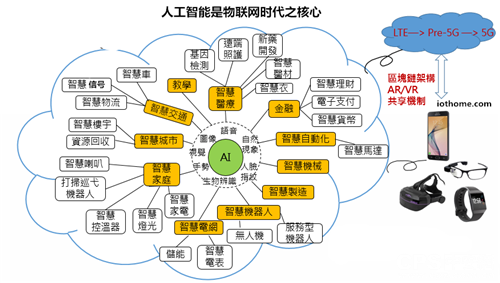
\includegraphics[width=0.6\textwidth]{AI20191218182305.png}
	\caption{人工智能是物联网时代之核心}
   \label{AI20191218182305Fig4}
\end{figure}

目前来看, 未来AI发展有八大新趋势
\begin{itemize}
\item  趋势一、\Circled{AI于各行业垂直领域应用具有巨大的潜力}

人工智能市场在零售、交通运输和自动化、制造业及农业等各行业垂直领域具有巨大的潜力. 而驱动市场的主要因素, 是人工智能技术在各种终端用户垂直领域的应用数量不断增加, 尤其是改善对终端消费者服务.当然人工智能市场要起来也受到IT基础设施完善、智能手机及智能穿戴式设备的普及.其中, 以自然语言处理(NLP)应用市场占AI市场很大部分. 随着自然语言处理的技术不断精进而驱动消费者服务的成长, 还有: 汽车信息通讯娱乐系统、AI机器人及支持AI的智能手机等领域.
\item  趋势二、\Circled{AI导入医疗保健行业维持高速成长}

由于医疗保健行业大量使用大数据及人工智能, 进而精准改善疾病诊断、医疗人员与患者之间人力的不平衡、降低医疗成本、促进跨行业合作关系. 此外AI还广泛应用于临床试验、大型医疗计划、医疗咨询与宣传推广和销售开发. 人工智能导入医疗保健行业从2016年到2022年维持很高成长, 预计从2016年的6.671亿美元达到2022年的79.888亿美元年均复合增长率为52.68\%.
%%%%%%%%%%%%%%%%%%%%%%%%%%%%%%
\begin{figure}[htbp]
	\centering
	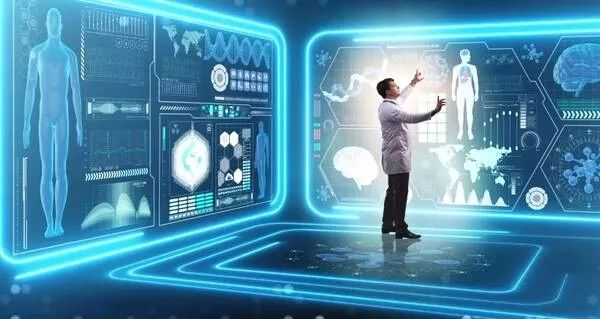
\includegraphics[width=0.5\textwidth]{AI20191218182524.jpg}
	\caption{人工智能是物联网时代之核心}
   \label{AI20191218182524}
\end{figure}

\item  趋势三、\Circled{AI取代屏幕成为新UI/UX接口}

过去从PC到手机时代以来, 用户接口都是透过屏幕或键盘来互动. 随着智能喇叭(SmartSpeaker)、虚拟/增强现实(VR/AR)与自动驾驶车系统陆续进入人类生活环境, 加速在不需要屏幕的情况下, 人们也能够很轻松自在与运算系统沟通. 这表示着人工智能透过自然语言处理与机器学习让技术变得更为直观, 也变得较易操控, 未来将可以取代屏幕在用户接口与用户体验的地位. 人工智能除了在企业后端扮演重要角色外, 在技术接口也可承担更复杂角色. 例如: 使用视觉图形的自动驾驶车, 透过人工神经网络以实现实时翻译, 也就是说, 人工智能让接口变得更为简单且更有智能, 也因此设定了未来互动的高标准模式.
\item  趋势四、\Circled{未来手机芯片一定内建AI运算核心}

现阶段主流的ARM架构处理器速度不够快, 若要进行大量的图像运算仍嫌不足, 所以未来的手机芯片一定会内建AI运算核心. 正如, 苹果将3D感测技术带入iPhone之后, Android阵营智能手机也将跟进导入3D感测相关应用.
\item  趋势五、\Circled{AI芯片关键在于成功整合软硬件}

AI芯片的核心是半导体及算法. AI硬件主要是要求更快指令周期与低功耗, 包括GPU、DSP、ASIC、FPGA和神经元芯片, 且须与深度学习算法相结合, 而成功相结合的关键在于先进的封装技术. 总体来说GPU比FPGA快, 而在功率效能方面FPGA比GPU好, 所以AI硬件选择就看产品供货商的需求考虑而定. 例如, 苹果的FaceID脸部辨识就是3D深度感测芯片加上神经引擎运算功能, 整合高达8个组件进行分析, 分别是红外线镜头、泛光感应组件、距离传感器、环境光传感器、前端相机、点阵投影器、喇叭与麦克风. 苹果强调用户的生物识别数据, 包含: 指纹或脸部辨识都以加密形式储存在iPhone内部, 所以不易被窃取.

\item  趋势六、 \Circled{使用人工智能的预测营销}

人工智能有助于预测用户的个性. 全球用户进行了数十亿次搜索. 搜索数据被保存在数据库中, 用于预测用户的人口位置、喜好、兴趣和职业等. 这有助于针对产品和服务定位到正确的客户.

\item  趋势七、\Circled{定制网站}


如何向不同用户展示具有个性化内容的同一网站?这在人工智能的帮助下也成为可能. 根据过去的搜索, 人口统计位置, 性别, 喜好, 人工智能可以定制网站, 并向用户显示他想看到的内容. 这在很大程度上改善了用户体验.
人工智能的市场价值具有巨大的净值空间. 随着商业营销概念的日益增多, 人工智能的市场价值也越来越多元化. 人工智能公司与商业营销合作, 获得了巨额利润. 人工智能的市场价值呈指数级增长, 预计未来几年还会增长.

\item  趋势八、\Circled{语音搜索}

未来几年, 语音搜索将完全超越文本搜索. 在人工智能和语音识别系统的帮助下, 用户仅仅使用自己的语音就可以发出各种命令. AI系统首先识别语音, 将它们从语音转换为文本, 并提供想得到的结果. 这意味着网站的内容应与人类对话交互过程相匹配.

\item  趋势九、\Circled{图像识别系统}

机器人技术和人工智能使人们很容易识别人、产品等的图像. 因此, 人工智能可以识别图像中的人, 并且更先进的系统能够收集消费者信息, 进一步用于决策.
%%%%%%%%%%%%%%%%%%%%%%%%%%%%%%
\begin{figure}[htbp]
	\centering
	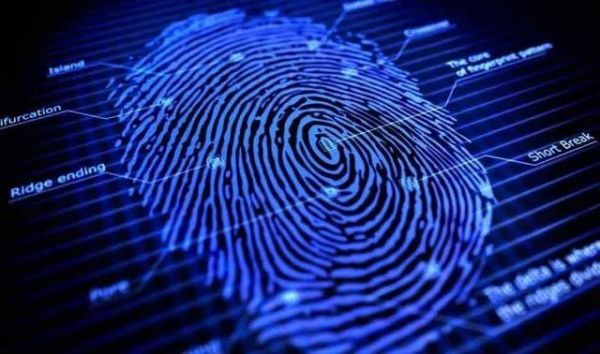
\includegraphics[width=0.5\textwidth]{AI20191218182642.jpg}
   \label{AI20191218182642}
\end{figure}
\item  趋势十、\Circled{AI自主学习是终极目标}

AI“大脑”变聪明是分阶段进行, 从机器学习进化到深度学习, 再进化至自主学习. 目前, 仍处于机器学习及深度学习的阶段, 若要达到自主学习需要解决四大关键问题. 首先, 是为自主机器打造一个AI平台;还要提供一个能够让自主机器进行自主学习的虚拟环境, 必须符合物理法则, 碰撞, 压力, 效果都要与现实世界一样;然后再将AI的“大脑”放到自主机器的框架中;最后建立虚拟世界入口(VR). 目前, NVIDIA推出自主机器处理器Xavier, 就在为自主机器的商用和普及做准备工作.
\item  趋势十一、\Circled{最完美的架构是把CPU和GPU(或其他处理器)结合起来}

未来, 还会推出许多专门的领域所需的超强性能的处理器, 但是CPU是通用于各种设备, 什么场景都可以适用. 所以, 最完美的架构是把CPU和GPU(或其他处理器)结合起来. 例如, NVIDIA推出CUDA计算架构, 将专用功能ASIC与通用编程模型相结合, 使开发人员实现多种算法.
\item  趋势十二、\Circled{AR成为AI的眼睛, 两者是互补、不可或缺}
 
未来的AI需要AR, 未来的AR也需要AI, 可以将AR比喻成AI的眼睛. 为了机器人学习而创造的在虚拟世界, 本身就是虚拟现实. 还有, 如果要让人进入到虚拟环境去对机器人进行训练, 还需要更多其它的技术.
\end{itemize}
%%%%%%%%%%%%%%%%%%%%%%%%%%%%%%
\begin{figure}[htbp]
	\centering
	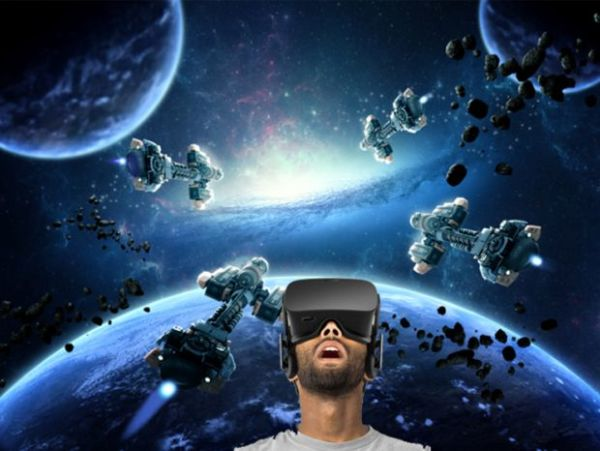
\includegraphics[width=0.5\textwidth]{AI20191218182713.jpg}
   \label{AI20191218182713}
\end{figure} 

来源:物联之家
%%%%%%%%%%%%%%%%%%%%%%%%%%%%%%%%%%%%
\subsection{达摩院2020十大科技趋势}
\begin{itemize}
\item  趋势一、\Circled{人工智能从感知智能向认知智能演进}

人工智能已经在“听、说、看”等感知智能领域已经达到或超越了人类水准, 但在需要外部知识、逻辑推理或者领域迁移的认知智能领域还处于初级阶段. 认知智能将从认知心理学、脑科学及人类社会历史中汲取灵感, 并结合跨领域知识图谱、因果推理、持续学习等技术, 建立稳定获取和表达知识的有效机制, 让知识能够被机器理解和运用, 实现从感知智能到认知智能的关键突破.

\item  趋势二、\Circled{计算存储一体化突破AI算力瓶颈}

冯诺伊曼架构的存储和计算分离, 已经不适合数据驱动的人工智能应用需求. 频繁的数据搬运导致的算力瓶颈以及功耗瓶颈已经成为对更先进算法探索的限制因素. 类似于脑神经结构的存内计算架构将数据存储单元和计算单元融合为一体, 能显著减少数据搬运, 极大提高计算并行度和能效. 计算存储一体化在硬件架构方面的革新, 将突破AI算力瓶颈.

\item  趋势三、\Circled{工业互联网的超融合}

5G、IoT设备、云计算、边缘计算的迅速发展将推动工业互联网的超融合, 实现工控系统、通信系统和信息化系统的智能化融合. 制造企业将实现设备自动化、搬送自动化和排产自动化, 进而实现柔性制造, 同时工厂上下游制造产线能实时调整和协同. 这将大幅提升工厂的生产效率及企业的盈利能力. 对产值数十万亿乃至数百万亿的工业产业而言, 提高5\%-10\%的效率, 就会产生数万亿人民币的价值.

\item  趋势四、\Circled{机器间大规模协作成为可能}

传统单体智能无法满足大规模智能设备的实时感知、决策. 物联网协同感知技术、5G通信技术的发展将实现多个智能体之间的协同——机器彼此合作、相互竞争共同完成目标任务. 多智能体协同带来的群体智能将进一步放大智能系统的价值: 大规模智能交通灯调度将实现动态实时调整, 仓储机器人协作完成货物分拣的高效协作, 无人驾驶车可以感知全局路况, 群体无人机协同将高效打通最后一公里配送.

\item  趋势五、\Circled{模块化降低芯片设计门槛}

传统芯片设计模式无法高效应对快速迭代、定制化与碎片化的芯片需求. 以RISC-V为代表的开放指令集及其相应的开源SoC芯片设计、高级抽象硬件描述语言和基于IP的模板化芯片设计方法, 推动了芯片敏捷设计方法与开源芯片生态的快速发展. 此外, 基于芯粒(chiplet)的模块化设计方法用先进封装的方式将不同功能“芯片模块”封装在一起, 可以跳过流片快速定制出一个符合应用需求的芯片, 进一步加快了芯片的交付.

\item  趋势六、\Circled{规模化生产级区块链应用将走入大众}

区块链BaaS(Blockchain as a Service)服务将进一步降低企业应用区块链技术的门槛, 专为区块链设计的端、云、链各类固化核心算法的硬件芯片等也将应运而生, 实现物理世界资产与链上资产的锚定, 进一步拓展价值互联网的边界、实现万链互联. 未来将涌现大批创新区块链应用场景以及跨行业、跨生态的多维协作, 日活千万以上的规模化生产级区块链应用将会走入大众.

\item  趋势七、\Circled{量子计算进入攻坚期}

2019年, “量子霸权”之争让量子计算在再次成为世界科技焦点. 超导量子计算芯片的成果, 增强了行业对超导路线及对大规模量子计算实现步伐的乐观预期. 2020年量子计算领域将会经历投入进一步增大、竞争激化、产业化加速和生态更加丰富的阶段. 作为两个最关键的技术里程碑, 容错量子计算和演示实用量子优势将是量子计算实用化的转折点. 未来几年内, 真正达到其中任何一个都将是十分艰巨的任务, 量子计算将进入技术攻坚期.

\item  趋势八、\Circled{新材料推动半导体器件革新}

在摩尔定律放缓以及算力和存储需求爆发的双重压力下, 以硅为主体的经典晶体管很难维持半导体产业的持续发展, 各大半导体厂商对于3纳米以下的芯片走向都没有明确的答案. 新材料将通过全新物理机制实现全新的逻辑、存储及互联概念和器件, 推动半导体产业的革新. 例如, 拓扑绝缘体、二维超导材料等能够实现无损耗的电子和自旋输运, 可以成为全新的高性能逻辑和互联器件的基础; 新型磁性材料和新型阻变材料能够带来高性能磁性存储器如SOT-MRAM和阻变存储器.

\item  趋势九、\Circled{保护数据隐私的AI技术将加速落地}

数据流通所产生的合规成本越来越高. 使用AI技术保护数据隐私正在成为新的技术热点, 其能够在保证各方数据安全和隐私的同时, 联合使用方实现特定计算, 解决数据孤岛以及数据共享可信程度低的问题, 实现数据的价值.

\item  趋势十、\Circled{云成为IT技术创新的中心}

随着云技术的深入发展, 云已经远远超过IT基础设施的范畴, 渐渐演变成所有IT技术创新的中心. 云已经贯穿新型芯片、新型数据库、自驱动自适应的网络、大数据、AI、物联网、区块链、量子计算整个IT技术链路, 同时又衍生了无服务器计算、云原生软件架构、软硬一体化设计、智能自动化运维等全新的技术模式, 云正在重新定义IT的一切. 广义的云, 正在源源不断地将新的IT技术变成触手可及的服务, 成为整个数字经济的基础设施.
\end{itemize}
%%%%%%%%%%%%%%%%%%%%%%%%%%%%%%%%%%%%
\section{AI的相关应用领域}
尽管目前不同人工智能的研究学派在理论基础、研究方法等方面还存在一定差异, 但这些并没有影响人工智能的发展, 反而使人工智能的研究更加客观、全面和深入.

今天, 被冠以智能的科技领域和社会现实数不胜数, 智能已成为一个极具价值的学术标签和商业标签, 并在科技进步和社会发展中扮演着越来越重要的角色.

面对人工智能这样一个高度交叉的新兴学科, 其研究和应用领域的划分可以有多种不同方法. 这里采用了基于智能本质和作用的划分方法, 即从感知、思维、行为、学习; 计算智能、分布智能、智能机器、智能系统、智能应用等方面来进行讨论.
%%%%%%%%%%%%%%%%%%%%%%%%%%%%%%%%%%%%
\subsection{机器思维}
机器思维: 就是让计算机模仿并实现人的思维, 具有人类类似的思维能力, 以对感知到的外界信息和自己内部产生的信息进行思维性加工.
     包括: \uwave{推理、搜索、规划等方面的研究}.
%%%%%%%%%%%%%%%%%%%%%%%%%%%%%%%%%%%%
\subsubsection{推理和搜索}
%%%%%%%%%%%%%%%%%%%%%%%%%%%%%%%%%%%%
\paragraph{推理}

推理的概念: 推理是指按照某种策略从已知事实出发利用知识推出所需结论的过程.
\begin{itemize}
\item 推理的类型: 可根据所用知识的确定性, 将其分为:
\item 确定性推理, 也称二值推理, 指推理所使用的知识和推出的结论都是可以精确表示的, 其真值要么为真、要么为假. 确定性推理主要是基于\textbf{一阶经典逻辑}. 它能解决的问题很有限.
\item \textbf{不确定性推理}, 指推理所使用的知识和推出的结论可以是不确定的. 所谓不确定性是对非精确性、随机性、模糊型和非完备性的统称. 不确定性推理主要基于非经典逻辑和概率等. 非一阶经典逻辑是泛指\textbf{除一阶经典逻辑以外的其他各种逻辑}, 如多值逻辑、模糊逻辑、模态逻辑、概率逻辑、默认逻辑、次协调逻辑及泛逻辑等.
\item 推理的理论基础: 逻辑是一门研究人们思维规律的学科, 数理逻辑则是用数学的方法去研究逻辑问题.
\end{itemize}
最常用的不确定性推理方法: 基于可信度的确定性理论, 基于Bayes公式的主观Bayes方法, 基于概率的证据理论和基于模糊逻辑的模糊推理(可能性理论)等.

%%%%%%%%%%%%%%%%%%%%%%%%%%%%%%%%%%%%
\paragraph{搜索}

搜索的概念: 是指为了达到某一目标, 不断寻找推理线路, 以引导和控制推理, 使问题得以解决的过程.

搜索的主要问题: 人工智能最关心的是如何利用已有的有用信息来引导搜索过程, 尽快达到目标, 即启发式搜索方法.
\begin{itemize}
\item 搜索的类型:可根据问题的表示方式将其分为状态空间搜索和与/或树搜索两大类型.
\item 状态空间搜索是一种用\textbf{状态空间法}求解问题时的搜索方法.
\item 与/或树搜索是一种用\textbf{问题规约法}求解问题时的搜索方法.
   \begin{itemize}
    \item 状态空间的启发式搜索方法
    \item 与/或树的启发式搜索方法
  \end{itemize}
\end{itemize}
%%%%%%%%%%%%%%%%%%%%%%%%%%%%%%%%%%%%
\paragraph{规划}
%%%%%%%%%%%%%%%%%%%%%%%%%%%%%%%%%%%%
\subparagraph{规划的概念}
是指从某个特定问题状态出发, 寻找并建立一个操作序列, 直到求得目标状态为止的一个行动过程的描述.
%%%%%%%%%%%%%%%%%%%%%%%%%%%%%%%%%%%%
\subparagraph{规划的特点}
与一般问题求解技术相比, 规划更侧重于问题求解过程, 并且要解决的问题一般是真实世界的实际问题, 而不是抽象的数学模型.
\begin{example}
  第\ref{AIchap2}章的机器人移盒子、猴子摘香蕉等问题.
\end{example}
%%%%%%%%%%%%%%%%%%%%%%%%%%%%%%%%%%%%
\subparagraph{规划系统的例子}
斯坦福研究所的问题求解系统(Stanford Research Institute Problem Solver,  STRIPS), 是一种基于状态空间和F规则的规划系统. 它由以下3部分所组成:

    (1) 世界模型: 用一阶谓词公式表示, 它包括问题的初始状态和目标状态.

    (2) 操作符(即$F$规则): 它包括先决条件、删除表和添加表.

    (3) 操作方法: 它采用状态空间表示和中间---结局分析的方法. 其中, 状态空间包括初始状态、中间状态和目标状态; 中间---结局分析的每一步都选择能够缩小当前状态与目标状态之间的差距的先决条件可以满足的$F$规则执行, 直至到达目标为止.

%%%%%%%%%%%%%%%%%%%%%%%%%%%%%%%%%%%%
\subsection{机器感知}
机器感知是机器获取外界信息的主要途径, 也是机器智能的重要组成部分.
%%%%%%%%%%%%%%%%%%%%%%%%%%%%%%%%%
\begin{mydef}{机器感知}{1}
让计算机具有类似于人的感知能力, 如视觉、听觉、触觉、嗅觉、味觉.
\end{mydef}
下面主要介绍机器视觉、模式识别和自然语言理解.
\subsubsection{机器视觉}
%%%%%%%%%%%%%%%%%%%%%%%%%%%%%%%%%%%%
%%%%%%%%%%%%%%%%%%%%%%%%%%%%%%%%%
\begin{mydef}{计算机视觉}{1}
用计算机来实现或模拟人类的视觉功能, 其主要研究目标是使计算机具有通过二维图像认知三维环境信息的能力.
\end{mydef}

重要性: 在人类感知到的外界信息中, 有80\%以上是通过视觉得到的.

视觉: 不仅仅指对光信号的感受, 它包括了对视觉信息的获取、传输、处理、存储与理解的全过程.

视觉系统: 人类视觉系统的功能是通过眼睛与大脑共同实现的. 人们视野中的物体在可见光的照射下, 先在眼睛的视网膜上形成图像, 然后由感光细胞转换成神经脉冲信号, 再经神经纤维传入大脑皮层, 最后由大脑皮层对其进行处理与理解.
%%%%%%%%%%%%%%%%%%%%%%%%%%%%%%%%%%%%%%%%
\begin{example}
设$p$为一物体. 两个透镜的轴线是平行的. $f$为两透镜与图像平面的距离, 即为焦距. $b$为两透镜轴线在基线上的距离, 即为两眼的距离. $l$和$m$分别是$p$点与左、右透镜轴线的距离. $a$和$c$分别是图像平面上的左、右图像与其相应透镜轴线上的距离.
从两个相似三角形, 可得到下式:
\begin{align}
  \frac d l=\frac {d+f}{l+a},  \frac d m=\frac {d+f}{m+c},  d=\frac{f\times b}{a+c}
\end{align}
\end{example}
已知$b=l+m$, 由上式可得观察者双眼至物体的距离:
\begin{figure}[htbp]
	\centering
	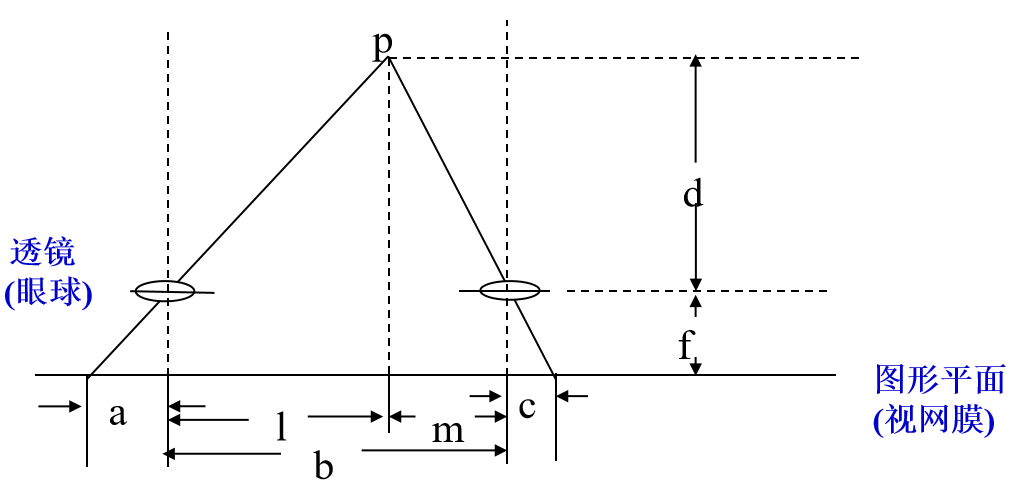
\includegraphics[width=0.75\textwidth]{Examp2019120101.png}
	\caption{示意图}
   \label{AI:Fig3}
\end{figure}
由于双眼的距离$b$为已知, 焦距$f$也是确定的, 因此$d$是可直接计算出来的.
%%%%%%%%%%%%%%%%%%%%%%%%%%%%%%%%%
\vspace{0.5cm}
\begin{mydef}{模式识别}{1}
是指让计算机能够对给定的事务进行鉴别, 并把它归入与其相同或相似的模式中.
被鉴别的事物可以是物理的、化学的、生理的, 也可以是文字、图像、声音等.
\end{mydef}
%%%%%%%%%%%%%%%%%%%%%%%%%%%%%%%%%%%%
\subparagraph{模式识别的一般过程}

\indent
      (1) 采集待识别事物的模式信息;

      (2) 对其进行各种变换和预处理, 从中抽出有意义的特征或基元, 得到待识别事物的模式;

      (3) 与机器中原有的各种标准模式进行比较, 完成对待识别事物的分类识别;

      (4) 输出识别结果.

自然语言处理包括的主要内容:
\begin{itemize}
\item 机器翻译: 把一种自然语言翻译成另外一种自然语言.
\item 自然语言理解主要研究如何使计算机能够理解和生成自然语言.

    理解的语言类型: 声音语言、书面语言.

    主要步骤: 语音分析、词法分析、句法分析、语义分析、语用分析.
\end{itemize}

自然语言理解的意义

该研究不仅对智能人机接口有着重要的实际意义, 而且对不确定人工智能的研究也具有重大的理论价值. 有学者指出: 人工智能如果不能用自然语言作为其知识表示基础, 建立起不确定人工智能的理论和方法, 人工智能也就永远实现不了跨越的梦想.
%%%%%%%%%%%%%%%%%%%%%%%%%%%%%%%%%%%%
\subsection{机器行为}
\vspace{0.5cm}
\begin{mydef}{机器行为}{1}
就是让计算机能够具有像人那样地行动和表达能力, 如走、跑、拿、说、唱、写画等.
\end{mydef}
机器行为则可看作智能系统的输出部分. 主要讨论内容为智能控制、智能检索和智能机器人等.
%%%%%%%%%%%%%%%%%%%%%%%%%%%%%%%%%%%%
\vspace{0.5cm}
\begin{mydef}{智能控制}{1}
是指那种无需或需要尽可能少的人工干预就能独立的驱动智能机器实现其目标的控制过程. 它是人工智能技术与传统自动控制技术相结合的产物.
\end{mydef}
\begin{itemize}
\item 智能控制系统: 是指那种能够实现某种控制任务, 具有自学习、自适应和自组织功能的智能系统. 从结构上, 它由传感器、感知信息处理模块、认知模块、规划和控制模块、执行器和通信接口模块等主要部件所组成.
\item 智能控制的主要应用领域: 智 能机器人系统、计算机集成制造系统(CIMS)、复杂工业过程的控制系统、航空航天控制系统、社会经济管理系统、交通运输系统、环保及能源系统等.
\end{itemize}
%%%%%%%%%%%%%%%%%%%%%%%%%%%%%%%%%%%%
%%%%%%%%%%%%%%%%%%%%%%%%%%%%%%%%%
\begin{mydef}{智能检索}{1}
是指利用人工智能的方法从大量信息中尽快找到所需要的信息或知识.
\end{mydef}

智能检索的重要性: 目前, 在各种数据库中, 尤其是互联网上存放着大量的、甚至是海量的信息或知识. 面对这种信息海洋, 如果还用传统的人工方式进行检索, 已很不现实.

智能检索系统须解决的主要问题:

(1) 具有一定的自然语言理解能力, 能理解用自然语言提出的各种询问;

(2) 具有一定的推理能力, 能够根据已知的信息或知识, 演绎出所需要的答案;

(3) 系统应拥有一定的常识性知识, 以补充学科范围的专业知识. 系统根据这些常识, 将能演绎出更一般询问的一些答案.
%%%%%%%%%%%%%%%%%%%%%%%%%%%%%%%%%%%%
机器人(Robots)和机器人学: 机器人(Robots)是一种可再编程的多功能操作装置. 机器人学是在电子学、人工智能、控制论、系统工程、精密机械、信息传感、仿生学、以及心理学等多种学科或技术发展的基础上形成的一种综合性技术学科.

\uwave{机器人研究的意义}: 机器人既是人工智能的研究对象, 同时又是人工智能的试验场地, 人工智能的所有技术几乎都可以在这个领域得到应用.

\uwave{机器人的发展过程}:  经历了遥控、程序、自适应、智能机器人、情感机器人. 人工智能的主要研究对象是智能机器人和情感机器人.

\uwave{智能机器人具有的能力}: 感知能力、思维能力和行为能力的机器人. 这种机器人能够主动的适应外界环境变化, 并能够通过学习丰富自己的知识、提高自己的工作能力.

\uwave{情感机器人}: 是一种具有情感(爱、恨…)和情绪(喜、怒、哀、乐…)功能新一代机器人.
%%%%%%%%%%%%%%%%%%%%%%%%%%%%%%%%%%%%
\subsection{计算智能}
计算智能(Computational Intelligence, CI)是借鉴仿生学的思想, 基于人们对生物体智能机理的认识, 采用数值计算的方法去模拟和实现人类的智能. 计算智能的三大基本领域包括神经计算、进化计算、模糊计算.
%%%%%%%%%%%%%%%%%%%%%%%%%%%%%%%%%%%%
\subsubsection{神经计算}
\begin{mydef}{神经计算}{1}
亦称神经网络(Neural Network, NN), 它是通过对大量人工神经元的广泛并行互联所形成的一种人工网络系统, 用于模拟生物神经系统的结构和功能.
\end{mydef}
主要研究内容:包括人工神经元的结构和模型, 人工神经网络的互连结构和系统模型, 基于神经网络的联结学习机制等.
\begin{itemize}
\item 人工神经元: 是指用人工方法构造单个神经元, 它有抑制和兴奋两种工作状态, 可以接受外界刺激, 也可以向外界输出自身的状态, 用于模拟生物神经元的结构和功能, 是人工神经网络的基本处理单元.
\item 人工神经网络的互连结构(或称拓扑结构)是指单个神经元之间的连接模式, 它是构造神经网络的基础. 从互连结构的角度, 神经网络可分为前馈网络和反馈网络两种主要类型.
\item 网络模型是对网络结构、连接权值和学习能力的总括. 最常用的有传统的感知器模型, 具有误差前向传播功能的前向传播网络模型, 采用反馈连接方式的反馈网络模型等.
\item 神经网络具有自学习、自组织、自适应、联想、模糊推理等能力, 在模仿生物神经计算方面有一定优势. 目前, 神经计算的研究和应用已渗透到许多领域, 如机器学习、专家系统、智能控制、模式识别等.
\end{itemize}
%%%%%%%%%%%%%%%%%%%%%%%%%%%%%%%%%%%%
\subsubsection{进化计算}
\begin{mydef}{进化计算}{1}
是一种模拟自然界生物进化过程与机制, 进行问题求解的自组织、自适应的随机搜索技术. 它以达尔文进化论的“物竞天择、适者生存”作为算法的进化规则, 并结合孟德尔的遗传变异理论, 将生物进化过程中的繁殖、变异、竞争和选择引入到了算法中, 是一种对人类智能的演化模拟方法.
\end{mydef}

进化计算的主要分支: 遗传算法、进化策略、进化规划和遗传规划四大分支. 其中, 遗传算法是进化计算中最初形成的一种具有普遍影响的模拟进化优化算法.

遗传算法的基本思想: (美国密执安大学霍兰德教授1962提出)是使用模拟生物和人类进化的方法来求解复杂问题. 它从初始种群出发, 采用优胜略汰、适者生存的自然法则选择个体, 并通过杂交、变异产生新一代种群, 如此逐代进化, 直到满足目标为止.
%%%%%%%%%%%%%%%%%%%%%%%%%%%%%%%%%%%%
\subsubsection{模糊计算}
\begin{mydef}{模糊计算}{1}
亦称模糊系统, 是通过对人类处理模糊现象的认知能力的认识, 用模糊集合和模糊逻辑去模拟人类的智能行为的. 模糊集合与模糊逻辑是美国加州大学扎德(Zadeh)教授1965年提出来的一种处理因模糊而引起的不确定性的有效方法.
\end{mydef}
\begin{mydef}{模糊}{1}
人们把那种因没有严格边界划分而无法精确刻画的现象称为模糊现象, 并把反映模糊现象的各种概念称为模糊概念.
\end{mydef}
\begin{example}
  “大”、“小”、“多”、“少”等.
\end{example}
\begin{itemize}
\item 模糊概念的表示: 通常是用模糊集合来表示的, 而模糊集合又是用隶属函数来刻画的. 一个隶属函数描述一个模糊概念, 其函数值为[0, 1]区间的实数, 用来描述函数自变量所代表的模糊事件隶属于该模糊概念的程度.
\item 模糊计算的争论: 一方面模糊逻辑存在一定缺陷; 另一方面它在推理、控制、决策等方面得到了非常广泛的应用.
\end{itemize}
%%%%%%%%%%%%%%%%%%%%%%%%%%%%%%%%%%%%
\subsection{机器学习}
\begin{itemize}
\item 机器学习就是让计算机能够像人那样自动地获取新知识, 并在实践中不断地完善自我和增强能力.
\item 机器学习是机器获取知识的根本途径, 同时也是机器具有智能的重要标志.
\item 机器学习有多种不同的分类方法, 如果按照对人类学习的模拟方式, 机器学习可分为符号学习和神经学习等.
\end{itemize}
%%%%%%%%%%%%%%%%%%%%%%%%%%%%%%%%%%%%
\subsubsection{符号学习}
\begin{itemize}
\item \uwave{符号学习}的概念: 是指从功能上模拟人类学习能力的机器学习方法, 它是一种基于符号主义学派的机器学习观点.
\item \uwave{符号学习}的类型: 可根据学习策略, 即学习中所使用的推理方法, 将其分为记忆学习、归纳学习、演绎学习等.
\item \uwave{记忆学习}也叫死记硬背学习, 它是一种最基本的学习方法, 原因是任何学习系统都必须记住它们所获取的知识, 以便将来使用.
\item \uwave{归纳学习}是指以归纳推理为基础的学习, 它是机器学习中研究得较多的一种学习类型, 其任务是要从关于某个概念的一系列已知的正例和反例中归纳出一个一般的概念描述.
\begin{example}
  示例学习和决策树学习.
\end{example}
\item \uwave{演绎学习}是指以演绎推理为基础的学习, 解释学习是一种演绎学习方法, 它是在领域知识的指导下, 通过对单个问题求解例子的分析, 构造出求解过程的因果解释结构, 并对该解释结构进行概括化处理, 得到一个可用来求解类似问题的一般性知识.
\end{itemize}
%%%%%%%%%%%%%%%%%%%%%%%%%%%%%%%%%%%%
\subsubsection{神经学习}
\begin{mydef}{神经学习}{1}
神经学习也称为连接学习, 它是一种基于人工神经网络的学习方法. 现有研究表明, 人脑的学习和记忆过程都是通过神经系统来完成的. 在神经系统中, 神经元既是学习的基本单位, 同是也是记忆的基本单位.
\end{mydef}

神经学习的类型:
\begin{itemize}
\item \uwave{感知器学习}实际上是一种基于纠错学习规则, 采用迭代的思想对连接权值和阈值进行不断调整, 直到满足结束条件为止的学习算法.
\item \uwave{BP网络学习}是一种误差反向传播网络学习算法. 这种学习算法的学习过程由输出模式的正向传播过程和误差的反向传播过程所组成, 其中, 误差的反向传播过程用于修改各层神经元的连接权值, 以逐步减少误差信号, 直至得到所期望的输出模式为止.
\item \uwave{Hopfield网络学习}实际上是要寻求系统的稳定状态, 即从网络的初始状态开始, 逐渐向其稳定状态过渡, 直至达到稳定状态为止. 至于网络的稳定性, 则是通过一个能量函数来描述的.
\end{itemize}
%%%%%%%%%%%%%%%%%%%%%%%%%%%%%%%%%%%%
\subsubsection{数据挖掘和知识发现}

\begin{mydef}{知识发现和数据挖掘}{1}
知识发现和数据挖掘是在数据库的基础上实现的一种知识发现系统. 它通过综合运用统计学、粗糙集理论、模糊数学、机器学习和专家系统等多种学习手段和方法, 从数据库中提炼和抽取知识, 从而可以揭示出蕴含在这些数据背后的客观世界的内在联系和本质原理, 实现知识的自动获取.
\end{mydef}

%%%%%%%%%%%%%%%%%%%%%%%%%%%%%%%%%%%%
\subparagraph{与传统数据库技术的区别}
传统数据库技术仅限于对数据库的查询和检索, 不能够从数据库中提取知识. 知识发现和数据挖掘以数据库作为知识源去抽取知识, 不仅可以提高数据库中数据的利用价值, 同时也为各种智能系统的知识获取开辟了一条新的途径.
%%%%%%%%%%%%%%%%%%%%%%%%%%%%%%%%%%%%
\subparagraph{发展}
随着大规模数据库和互联网的迅速发展, 知识发现和数据挖掘也从面向数据库的结构化信息的数据挖掘发展到面向数据仓库和互联网的海量、半结构化或非结构化信息的数据挖掘.
%%%%%%%%%%%%%%%%%%%%%%%%%%%%%%%%%%%%
\subsection{分布智能}

\begin{mydef}{分布智能}{1}
分布智能主要研究在逻辑上或物理上分布的智能系统之间如何相互协调各自的智能行为, 实现问题的并行求解.
\end{mydef}
分布智能的两个主要方向:
\begin{itemize}
\item 分布式问题求解主要研究如何在多个合作者之间进行任务划分和问题求解, 它一般是针对某一问题去创建一个能够进行合作求解的协作群体.
\item 多Agent系统主要研究如何在一群自主的Agent之间进行智能行为的协调, 它不限于单一目标, 可创建一个能够共同处理单个目标或多个目标的智能群体.
\item 多Agent系统的组成与工作: 它由多个自主Agent所组成, 其中的每个Agent都可以自主运行和自主交互, 即当一个Agent 需要与别的Agent合作时, 就通过相应的通信机制去寻找可以合作并愿意合作的Agent, 以共同解决问题.
\end{itemize}
%%%%%%%%%%%%%%%%%%%%%%%%%%%%%%%%%%%%
\subsection{智能系统}
\begin{mydef}{智能系统}{1}
智能系统可以泛指各种具有智能特征和功能的软硬件系统. 从这种意义上讲, 前面所讨论的不少研究内容都应以智能系统的形式来出现, 例如智能控制系统、智能制造系统、智能检索系统等. 这里主要介绍除前述研究内容以外的专家系统和智能决策支持系统.
\end{mydef}
%%%%%%%%%%%%%%%%%%%%%%%%%%%%%%%%%%%%
\subsubsection{专家系统}
\begin{mydef}{专家系统}{1}
专家系统是一种基于知识的智能系统, 它将领域专家的经验用知识表示方法表示出来, 并放入知识库中, 供推理机使用.
\end{mydef}

随着计算网络、多Agent、计算智能等技术的发展, 出现了模糊专家系统、神经网络专家系统、基于Web的专家系统、协同式专家系统和分布式专家系统等.
%%%%%%%%%%%%%%%%%%%%%%%%%%%%%%%%%%%%
\begin{figure}[htbp]
	\centering
	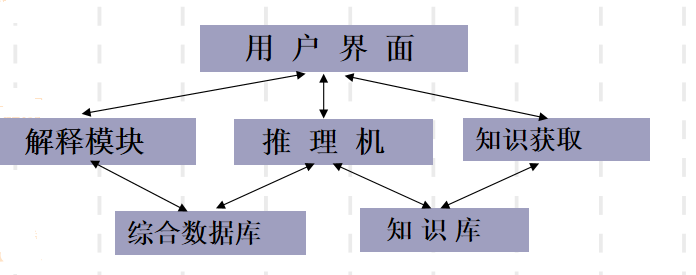
\includegraphics[width=0.65\textwidth]{tuili2019120102.png}
	\caption{专家系统结构}
   \label{AI:Fig4}
\end{figure}
%%%%%%%%%%%%%%%%%%%%%%%%%%%%%%%%%%%%
\subsubsection{智能决策支持系统}
\begin{mydef}{智能决策支持系统}{1}
智能决策支持系统是指那种在传统决策支持系统中增加了相应的智能部件的决策支持系统.
\end{mydef}

智能决策支持系统是把人工智能技术, 尤其是专家系统技术与决策支持系统相结合的产物, 具有很宽的应用范围和很好的应用前景.
\begin{figure}[htbp]
	\centering
	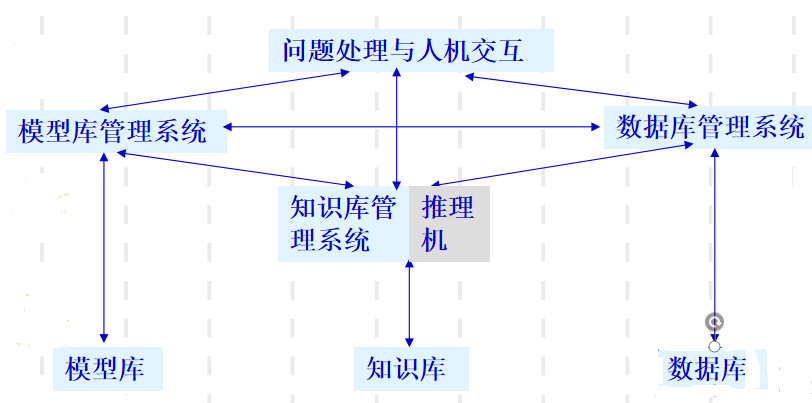
\includegraphics[width=0.65\textwidth]{turing320191203}
	\caption{智能决策支持系统}
   \label{AI:Fig4}
\end{figure}
%%%%%%%%%%%%%%%%%%%%%%%%%%%%%%%%%%%%
\subsection{人工心理与人工情感}
%%%%%%%%%%%%%%%%%%%%%%%%%%%%%%%%%%%%
\paragraph{\textbf{智能、情感和心理}}
\begin{itemize}
\item 智能: 是指感知、记忆、思维、学习、自适应、行为等能力
\item 情感: 指人对客观现实的态度的体验.
           \begin{itemize}
               \item 情绪(侧重于生理现象: 喜、怒、哀、乐…)
               \item 情感(侧重于价值判断: 爱、恨…)
               \item 情操(高级的情感现象: 道德、理智、审美…)
           \end{itemize}
\item 心理: 认知、情感、意志
           \begin{itemize}
               \item 认知: 实践活动中对认知信息的接收、编码、存储、提取、使用; 包括感知、思维、记忆等.
               \item 情感: …
               \item 意志: 自觉地确定目的, 并根据目的调节支配自身的行动, 克服困难, 去实现预定目标
           \end{itemize}
\end{itemize}
%%%%%%%%%%%%%%%%%%%%%%%%%%%%%%%%%%%%
\paragraph{\textbf{人工智能、人工情感和人工心理}}
\begin{itemize}
\item 人工智能: 研究、开发用于模拟、延伸和扩展人的智能的理论、方法、技术及应用系统的一门新的技术科学.
\item 人工情感: 人工情感(Artificial Emotion)是利用信息科学的手段对人类情感过程进行模拟、识别和理解, 使机器能够产生类人情感并与人类进行自然和谐地人机交互的研究领域.
\item 人工心理: 人工心理(Artificial Psychology)就是利用信息科学的手段,  对人的心理活动(着重是人的情感、意志、性格、创造)的更全面再一次人工机器(计算机、模型算法等)模拟, 其目的在于从心理学广义层次上研究人工情感、情感与认知、动机与情感的人工机器实现问题.
\end{itemize}
%%%%%%%%%%%%%%%%%%%%%%%%%%%%%%%%%%%%
\subsection{人工生命 }
人工生命(Artificial Life)是美国洛斯$\cdot$阿拉莫斯(Los Alamos)非线性研究中心克里斯$\cdot$兰顿(Chris Langton)于1987年在研究“混沌边沿”的细胞自动机提出的一个概念.

$\bullet$人工生命是通过对自然现象的模拟来研究行为如何变得智能、自适应的学科,以及复杂的行为如何产生. 研究内容就是要研究能够展示人类生命特征的人工系统. 即研究以非碳水化合物为基础的、具有人类生命特征的人造生命系统.

$\bullet$人工生命的研究目标就是要创造出具有人类生命特征的人工生命.
\begin{itemize}
\item 人工生命研究并不十分关心已经知道的以碳水化合物为基础的生命的特殊形式, 即“生命之所知(Lifeas we know it)”, 它主要是生物学研究的主题.
\item 人工生命最关心的是生命的存在形式, 即“生命之所能(Life as it could be)”. 生命之所能, 是人工生命研究所关心的主要问题.
\end{itemize}
按照这种观点, 如果能从具体的生命中抽象出控制生命的“存在形式”, 并且这种存在形式可以在另外一种物质中实现, 那么就可以创造出基于不同物质的另外一种生命——人工生命.

人工生命的主要研究内容主要包括\uwave{计算机进程、细胞自动机、人工脑和进化机器人}等. 其中, 进化机器人不同于传统意义上的机器人, 它是一种利用计算机和非有机物质构造出来的具有人类生命特征的人工生命实体.

%%%%%%%%%%%%%%%%%%%%%%%%%%%%%%%%%%%%
\subsection{自动推理}
近20年来, 几何定理机器证明的研究和实践有了很大的进展. 几何定理机器证明和非线性代数方程组作为主攻方向, 一方面是因为吴文俊先生在70年代的突出工作, 使中国在此方向上具有了领先的优势;另一方面, 这两个方向有鲜明的应用背景, 近年来在机器证明领域也确是十分活跃的, 值得重视. 由于传统的兴趣和多种原因, 几何定理的机器证明在自动推理的研究中占有重要的地位.

建立一个通用的几何解题方法, 成批地解决问题, 以至万理一证, 是历史上一些卓越科学家的梦想. 为此, 笛卡尔发明了坐标系; 莱布尼兹设想过推理机器; 希尔伯特在其名著(几何基础)中给出了一类几何命题的机械化定理. 电子计算机的出现推动了数学机械化. 50年代, 塔斯基用代数方法证明了初等几何的机械化的可能性. 到60年代, 斯拉格和莫色斯实现了符号积分, 代数与分析计算问题的机械化已经初具规模, 而几何定理的机器证明看来仍遥遥无期. 接着, 格兰特等提出用逻辑方法建立几何推理机, 科林斯等改进了塔斯基的代数方法. 直到1975年, 仍找不到能用计算机判定非平凡几何命题的有效算法. 吴文俊方法的提出给定理机器证明的研究带来勃勃生机. 用吴法可在微机上很快地证明困难的几何定理. 周咸青发展了吴法并把它实现为有效的通用程序, 证明了512条非平凡定理 (1981年开始), 写成英文专著. 这一进展是自动推理领域的一大突破, 被国际同行誉为革命性的工作.

\Circled{吴方法}的成功使几何定理机器证明研究活跃起来. 用代数方法证明几何定理的方向受到重视. 新的代数方法接连出现. 在国外, 周咸青等提出了用Grobner基方法构作几何定理机器证明的算法和程序并获得成功. 在国内, 洪家威提出了单点例证方法的理论设想, 但因复杂度太大不能实现. 张景中、杨路则提出数值并行方法, 在低档微机(甚至计算器)上实现了非平凡几何定理的机器证明和机器发明. 数值并行方法的优点是所需内存极小, 且易于并行化. 所有这些方法都属于代数方法. 它们的提出和实现丰富了几何定理机器证明的研究. 但与吴法相比, 没有大的新突破. 代数方法不能使人满意的是, 它所给出的"证明"是关于大多项式的繁复的计算, 人难于理解其几何意义, 也难于检验其是否正确. 能否让计算机生成人能理解和易于检验的简明巧妙的证明, 即所谓可读证明, 是对自动推理和人工智能领域的一个挑战性的课题. 一些著名的科学家认为, 机器证明的基本思想是以量的复杂取代质的困难, 这就很难想象用机器生成可读证明. 国外一些学者从60年代即致力于几何定理可读证明自动生成的研究, 30多年来进展不大, 未能给出哪怕是一小类非平凡几何定理的机器证明的有效算法和程序. 作者以多年来所发展的几何新方法为基本工具, 并提出了消点思想, 和周咸青、高小山合作, 于1992年突破了这一困难, 实现了几何定理可读证明的自动生成. 这一新方法既不以坐标为基础, 也不同于传统的综合方法, 而是一个以\textbf{几何不变量}为工具, 把几何、代数、逻辑和人工智能方法结合起来所形成的开放系统. 它选择几个基本的几何不变量和一套作图规则, 并且建立一系列与这些不变量和作图规则有关的消点公式. 当命题的前提以作图语句的形式输入时, 程序可调用适当的消点公式把结论中的约束点逐个消去, 最后达到水落石出. 消点的过程纪录与消点公式相结合, 就是一个具有几何意义的证明. 此算法对可构造等式型几何命题是完全的, 但其应用范围不限于这一类命题. 基于此法所编的程序, 已在微机上对数以百计的困难的几何定理完全自动地生成了简短的可读证明, 其效率也比其他方法为高. 随所用的几何量的不同, 它能生成面积法、向量法、复数法和全角法等多种风格的证明, 也能用于立体几何. 杨路、高小山、周咸青与作者合作, 把消点法用于非欧几何可读证明的自动生成也获得成功, 并得到一批非欧几何新定理. 消点法也可用于几何计算和公式推导. 基于几何量和消点思想的新原理的建立, 像是打开了几何定理机器求解的一个矿床. 它也使几何定理机器证明的成果在数学教育中的应用有了现实可能. 这一成果被国际同行誉为使计算机能像处理算术那样处理几何的发展道路上的里程碑, 是自动推理领域30年来最重要的工作. 在多数情形下, 消点法也可用笔纸证明不平凡的定理. 它结束了两千年来几何证题无定法的局面, 把初等几何解题法从四则杂题的层次推进到代数方程的阶段.

以吴方法为代表的代数方法仅仅能够判断几何命题的成立与否, 证明的过程十分复杂, 而且需要进行大量的数值计算和符号计算, 这与传统几何证明的简洁明了大相径庭. 人们难以读懂这种方法生成的证明, 往往只能得出命题真假的结论, 因此很多人难以接受这种证明的风格. 如何生成让人容易读懂的几何证明过程这一问题成为科学家面临的又一个严峻的挑战.  1992年, 中科院院士张景中教授以其多年研究的面积法为基础, 提出了几何定理机器证明的新方法, 基于几何不变量的消点法. 随后, 它与周咸青、高小山合作完善了该方法, 并编写了程序, 终于成功的利用计算机对大量非平凡的几何命题生成了简洁易读的几何证明, 这一杰出的工作被誉为计算机处理几何问题的里程碑.  消点法包括一组构图规则、一组几何不变量以及一组消点公式. 该方法的基本思想是:利用构图规则将欲证几何命题中涉及的图形构造出来, 并在构图的过程中生成关于点的约束条件, 同时将欲求证的命题表示成图中几何量的等式的形式, 然后利用消点公式, 按照点在作图时出现的相反顺序, 依次从结论等式中消去, 最终结论等式会化为显然成立的等式. 后来, 杨路教授又将消点法拓展到非欧几何, 成功的证明和发现了大量的新的非欧几何定理. 李洪波博士、杨海圈博士也在面积不变量的基础上提出用向量法实现几何定理的可读证明, 即Clifford代数法, 也取得了很好的效果.

近年来, 国外一再提出新的思路和算法, 欧共体还投资数百万美元组织项目专门研究非线性代数方程组的解法, 但均无突破性进展. 最近, 基于我们提出并加以完善的新的理论和算法———\textbf{结式矩阵法}, 符红光编写了代数方程组符号求解和机器证明的MAPLE程序.  \index{结式矩阵法}

机器证明的成果, 特别是非线性代数方程组理论与算法的研究成果, 将在数学、物理和工程技术中得到更多的应用. 目前, 在几何定理机器证明方面, 中国处于国际领先地位.

在非线性代数方程组研究领域, 竞争激烈, 中国已进入先进行列, 但还不能说领先.

在数学机械化软件开发方面, 由于起步晚、队伍小和资金不足等原因, 中国远不及欧美先进国家. 要把力量集中到非线性代数方程组的方向上来, 特别应加强对实用而有效的算法的研究.

在数学机械化推广应用方面, 也应投入力量, 发挥我国在理论与算法方向的优势, 在软件开发方面赶超先进. 在几何定理机器证明成果的基础上, 开发高智能的教育软件和自主版权的符号演算软件, 为中国科技、教育事业作出贡献(\href{https://www.maplesoft.com.cn/}{MAPLE},
\href{https://www.wolfram.com/}{Mathematica}, Maxima, Magma, REDUCE, Macsyma).
%%%%%%%%%%%%%%%%%%%%%%%%%%%%%%%%%%%%
\subsection{图神经网络——Open Graph Benchmark}
Jure Leskovec 教授在 NeurlPS 2019 大会演讲中宣布开源 Open Graph Benchmark (\href{http://ogb.stanford.edu}{百万量级OGB基准测试数据集}), 这是图神经网络建模统一基准迈出的重要一步, 是一个公认的基准测试数据集.

图神经网络是近来发展较快的机器学习分支领域. 通过将非结构数据转换为结构化的节点和边的图, 然后采用图神经网络进行学习, 往往能够取得更好的效果.
采用的方法往往是针对较小的、缺乏节点和边特征的数据集上进行的, 因此, 在这些数据集上取得的模型性能很难说是最好的, 也不一定可靠.

在 NeurlPS 2019 大会的图表示学习演讲中, Jure Leskovec 宣布开源图神经网络的通用性能评价基准数据集 OGB(Open Graph Benchmark). 通过这一数据集, 可以更好地评估模型性能等方面的指标.
\href{http://ogb.stanford.edu}{项目地址.}  \href{https://slideslive.com/38921872/graph-representation-learning-3}{图表示学习演讲合集}
%%%%%%%%%%%%%%%%%%%%%%%%%%%%%%%%%%%%
\subsection{工业4.0}
工业4.0最初在2011年由德国提出, 是指为促进工业制造数字化而制定的高科技项目战略, 从而打造完全自动化的制造行业. 目前, 工业4.0已经应用了最先进的科学技术:云计算、物联网、大数据、射频识别、协同开发等. 其中以物联网技术和大数据技术最为知名.

%%%%---------------------------------------------
\subsubsection{物联网技术与工业4.0}

物联网(Internet of Things, 简称IoT)最初由美国麻省理工学院工业自动识别中心的创始人凯文阿什顿在1999年提出, 指将一切通过高度智能化的交互系统连接, 从而形成自动化的世界.
这里的“智能”指利用先进的通信和互联网技术, 有效处理信息, 并形成“智能产业”. 物联网设备之间的交互动作, 让它们彼此获得信息, 使得设备自身可以监控业务流程、提高生产效率, 进而节省成本, 做出更好地决策.
物联网技术可以被分为四个阶段:

1) \uwave{数据传感阶段}:工业生成的数据通过传感器感测, 并收集传输到最近的基站等待处理;

2) \uwave{整理加工阶段}:对数据进行整理和处理, 并根据需要进行相应转换;

3) \uwave{预处理阶段}:利用边缘技术处理系统在数据传输到中心前进行预处理;

4) \uwave{存储维护阶段}:生成的数据被存储维护, 为后续分析建立基础;

物联网技术的四个阶段说明, 具有高度感测技术的自动化装置是工业物联网的基础组成部分, 这些智能机器的操作将增加工业生产的灵活性, 影响生产者对智能管理的依赖性, 并为行业发展设定新的标准.
物联网技术能满足数字市场的快速发展和消费者需求的不断增加, 在不需要人工干预的情况下, 及时、准确地完成分配的工作. 使用物联网的行业运营效率更高, 更能了解客户的需求, 最终提高盈利能力.
%%%%---------------------------------------------
\subsubsection{大数据与工业4.0}

工业发展导致系统中出现了巨大的数据流, 这些数据的保护、处理和维护成为人们关注的焦点, 大数据技术(Big Data Technology, 简称BDT)由此而生. 大数据最初来自IBM数据科学家, 从字面上讲, 意味着\uwave{大量信息的数据集合}, 它是一个分析海量数据的概念.
大数据这个概念有五个维度:

1) 体量:大数据代表数据数量上远比之前庞大;

2) 多样:不同的数据源, 生成了不同结构的数据;

3) 速度:数据生成的速度快, 分析处理的速度也快;

4) 真实:数据的真实性是分析的前提;

5) 价值:通过分析数据得到的行动是有价值的;

目前, 大数据已经成为各种业务数字化的基础, 它在收集、传输、分析和使用大量实时数据的同时, 生成的信息提供了智能流程的改进思路, 从而保障工业生产高效、无故障地执行. 适当收集和分析大数据将提高产品制造、供应链管理、物流和风险管理等多个部门的竞争力.

VUCA(发音近似于乌卡, 所以也用“乌卡”代表)战略指的是前言中提到的易变性、不确定性、复杂性和模糊性, 最初的VUCA战略发源于军事领域, 美军在20世纪90年代, 引用来描述冷战结束后的越发不稳定的、不确定的、复杂、模棱两可和多边的世界. 但是现在已经广泛应用于商业分析中. VUCA战略通过分析预期的发展风险因素, 并对这些情况加以准备, 从而在竞争激烈的商业世界中生存.

VUCA战略具有如下四个维度:

\Circled{易变性(Volatility)}: 指商业环境中的极端和快速变化. 这些变化的速度、数量和幅度可以反映它在商业环境中的波动程度. 产生易变性的原因往往是已知的, 比如价格的易变性会导致供应链的风险, 商品供给的易变性将导致公司无法满足消费者需求;

\Circled{不确定性(Uncertainty)}: 由于易变性的存在, 在缺乏了解的时候将会产生不确定性, 从而导致未来不可预测, 影响长期发展. 在商业环境中, 可能引起不确定性的因素包括: 用户需求、偏好的变化, 新政策的提出, 新产品对旧产品的替代等;

\Circled{复杂性(Complexity)}: 复杂性的产生来自两个方面, 一是工业化的快速发展, 使企业内部相互联系的网络和程序逐渐复杂, 二是外部的商业环境的不确定性导致决策的复杂性. 外包活动(如会计核算、市场营销和计算机辅助设计业务)的引入, 导致复杂性更加普遍;

\Circled{模糊性(Ambiguity)}: 在商业行动中, 模糊性表现无法清晰陈述、无法准确评估概率以及无法描述潜在结果的多样性, 当新产品或者新计划被引入市场时, 模糊性出现的可能性更高.
\begin{remark}
模糊数学中提到的不确定性和模糊性的含义不用于上述机器学习中的相应概念.
\end{remark}
%%%%---------------------------------------------
\subsubsection{机器学习下的VUCA战略}
在这一部分中, 介绍几种常用的机器学习算法并简要描述它们的原理, 并举例说明它们在工业4.0的VUCA战略的现实应用.

(1) \Circled{线性回归模型}: 线性回归是回归算法中一种有监督的机器学习算法, 它根据给定的变量来预测结果, 得到两者的线性关系. 常用的线性回归模型有两种, 分别是单个变量的简单线性和多变量的多元线性回归.
线性回归模型主要解决VUCA战略的易变性和不确定性问题. 谷歌公司的应用软件已经利用线性模型分析特定道路的历史数据, 来预测交通状况. 一些金融从业人员利用波动率指标建立线性模型来预测金融市场的波动性, 并证明该方法优于传统的移动平均法.

(2) \Circled{Logistic回归模型}: 是分类算法中一种有监督的机器学习算法, 以给定的变量作为输入值, 以0或1、是或否、真或假等离散值预测输出结果. 虽然是回归模型, 但解决的是分类问题, 通过给出预测数据所属类的概率来完成判别.
Logistic回归模型主要解决VUCA战略的复杂性和模糊性问题. 医疗行业用这个方法将病人分为关键诊断和非关键诊断类别, 金融行业据此建立预警模型, 根据过去的债务、违约情况和收入, 判断用户是否会在业务中违约. 回归算法有效地处理了复杂和模糊的风险因素, 预测结果具有较高的精度.

(3) \Circled{决策树模型}: 一种有监督的机器学习算法, 分为\uwave{分类算法}和\uwave{回归算法两类}. 数据集被分为具有相同类别的较小部分, 直到所有的数据都被分类, 且节点是最终的决策节点. 决策树由熵、信息增益来构成, 以预测事件的不确定性程度.
决策树模型主要解决VUCA战略中的不确定性和模糊性问题. 例如, 大型工业项目由于规划设计复杂, 且参与的群体多样, 存在很大的不确定性, 利用决策树模型可以对这些不确定因素进行分类, 提前预测风险.

(4) \Circled{随机森林模型}: 一种有监督的机器学习算法, 通过随机收集决策树来预测期望的结果, 从而创造“森林”, 随着决策树生长, 每个决策树都可以对新对象分类并投票, 最高票数将对随机森林的过程分类.
随机森林模型主要解决VUCA战略中的模糊性问题. 它有助于估计公司不稳定的业务绩效指标, 如预测机械零件故障的可能性、估算市场的盈利能力并最小化风险, 在预测灾害损失方面也有应用, 且效果优于其他机器学习算法.

(5) \Circled{支持向量机模型}: 分类算法范畴下的有监督机器学习算法, 通过生成\textbf{一个平面或者决策边界}将样本分成不同的类, 数据样本点根据不同的特征进行分类, 每个点都有不同的坐标作为支持向量.
支持向量机模型主要处理易变性、复杂性和不确定性问题. 供应链管理系统的需求预测、工业材料风险对冲模型等都涉及到了这些内容.

工业4.0通过物联网和大数据技术实现自动化数据交换, 通过云计算实现数据存储和处理, 通过认知计算帮助人类决策. 它降低了人力成本, 简化了业务流程, 提高了生产预测的准确性. 这些改进将显著提高生产效率和收入, 有助于经济增长.
然而, 工业4.0的进程中仍存在易变性、不确定性、复杂性和模糊性问题, 这些问题影响了工业发展进程, 需要得到合理的解决. 机器学习技术可以让智能设备在不需要人工编程的情况下做出决定, 从而减少不确定因素导致的风险, 在未来将被广泛应用.
%%%%---------------------------------------------
\subsubsection{基于算法的工业智能平台}

将成为应用场景的重要基石.
不同工业行业有各自独特的行业门槛, 每个工业场景在不同行业、不同企业中的需求差异较大.
人工智能与制造业深度融合的路径就是将信息技术与工业场景应用端结合.
将核心工艺模型化、算法化、代码化的工业智能算法平台面向工业场景, 可以为底层应用提供便捷的开发服务.
然而市面上有更智能的算法平台, 例如中机云集团的智能开发者平台, 无需编码一拖一拽即可快速生成应用程序的工具, 可以降低企业应用开发人力成本, 从而帮助企业实现降本增效、灵活迭代.
%%%%%%%%%%%%%%%%%%%%%%%%%%%%%%%%%%%%
\begin{figure}[htbp]
	\centering
	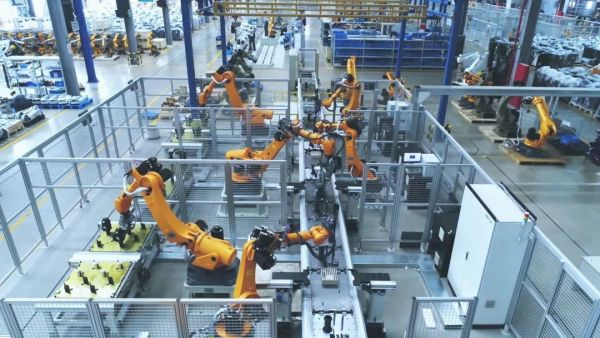
\includegraphics[width=0.456\textwidth]{BG20200306160800.jpg}
	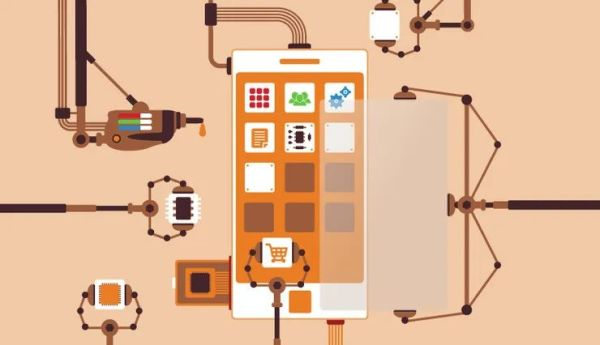
\includegraphics[width=0.45\textwidth]{AID20200306160821.jpg}
	\caption{基于大数据的工业智能的场景和智能开发者平台(中机云集团)}
   \label{AI:Fig4}
\end{figure}
%%%%%%%%%%%%%%%%%%%%%%%%%%%%%%%%%%%%


%%%%%%%%%%%%%%%%%%%%%%%%%%%%%%%%%%%%
\section{人工智能的典型应用  }
从理论到技术, 从产品到工程, 从家庭到社会, 从地下到太空, 智能无处不在, 人工智能的应用领域已非常广泛.
\begin{example}
    智能CAD、智能CAI、智能产品、智能家居、智能楼宇、智能社区、智能网络、智能电力、智能交通、智能控制、智能优化和智能空天技术等.
\end{example}

下面简单介绍其中的典型应用.
%%%%%%%%%%%%%%%%%%%%%%%%%%%%%%%%%%%%
\subsection{\textbf{博弈}}
\begin{itemize}
\item 博弈的概念: 是一个有关对策和斗智问题的研究领域. 例如, 下棋、打牌、战争等这一类竞争性智能活动都属于博弈问题.
\item 博弈的例子: 国际上对博弈的研究主要以下棋为对象, 其中代表性成果是IBM公司研制的IBM超级计算机“深蓝”和“小深”. 国内, 2006.8.9在北京举办的首届中国象棋人机大赛中, 计算机以3胜5和2负(比分11:9)的微弱优势战胜人类象棋大师.
\item 研究博弈的目的: 不完全是为了让计算机与人下棋, 而主要是为了给人工智能研究提供一个试验场地, 同时也为了证明计算机具备智能.
试想, 连国际象棋世界冠军都能被计算机战败或者平局, 可见计算机所具备了何等的智能水平.
\end{itemize}
\begin{figure}[htbp]
	\centering
	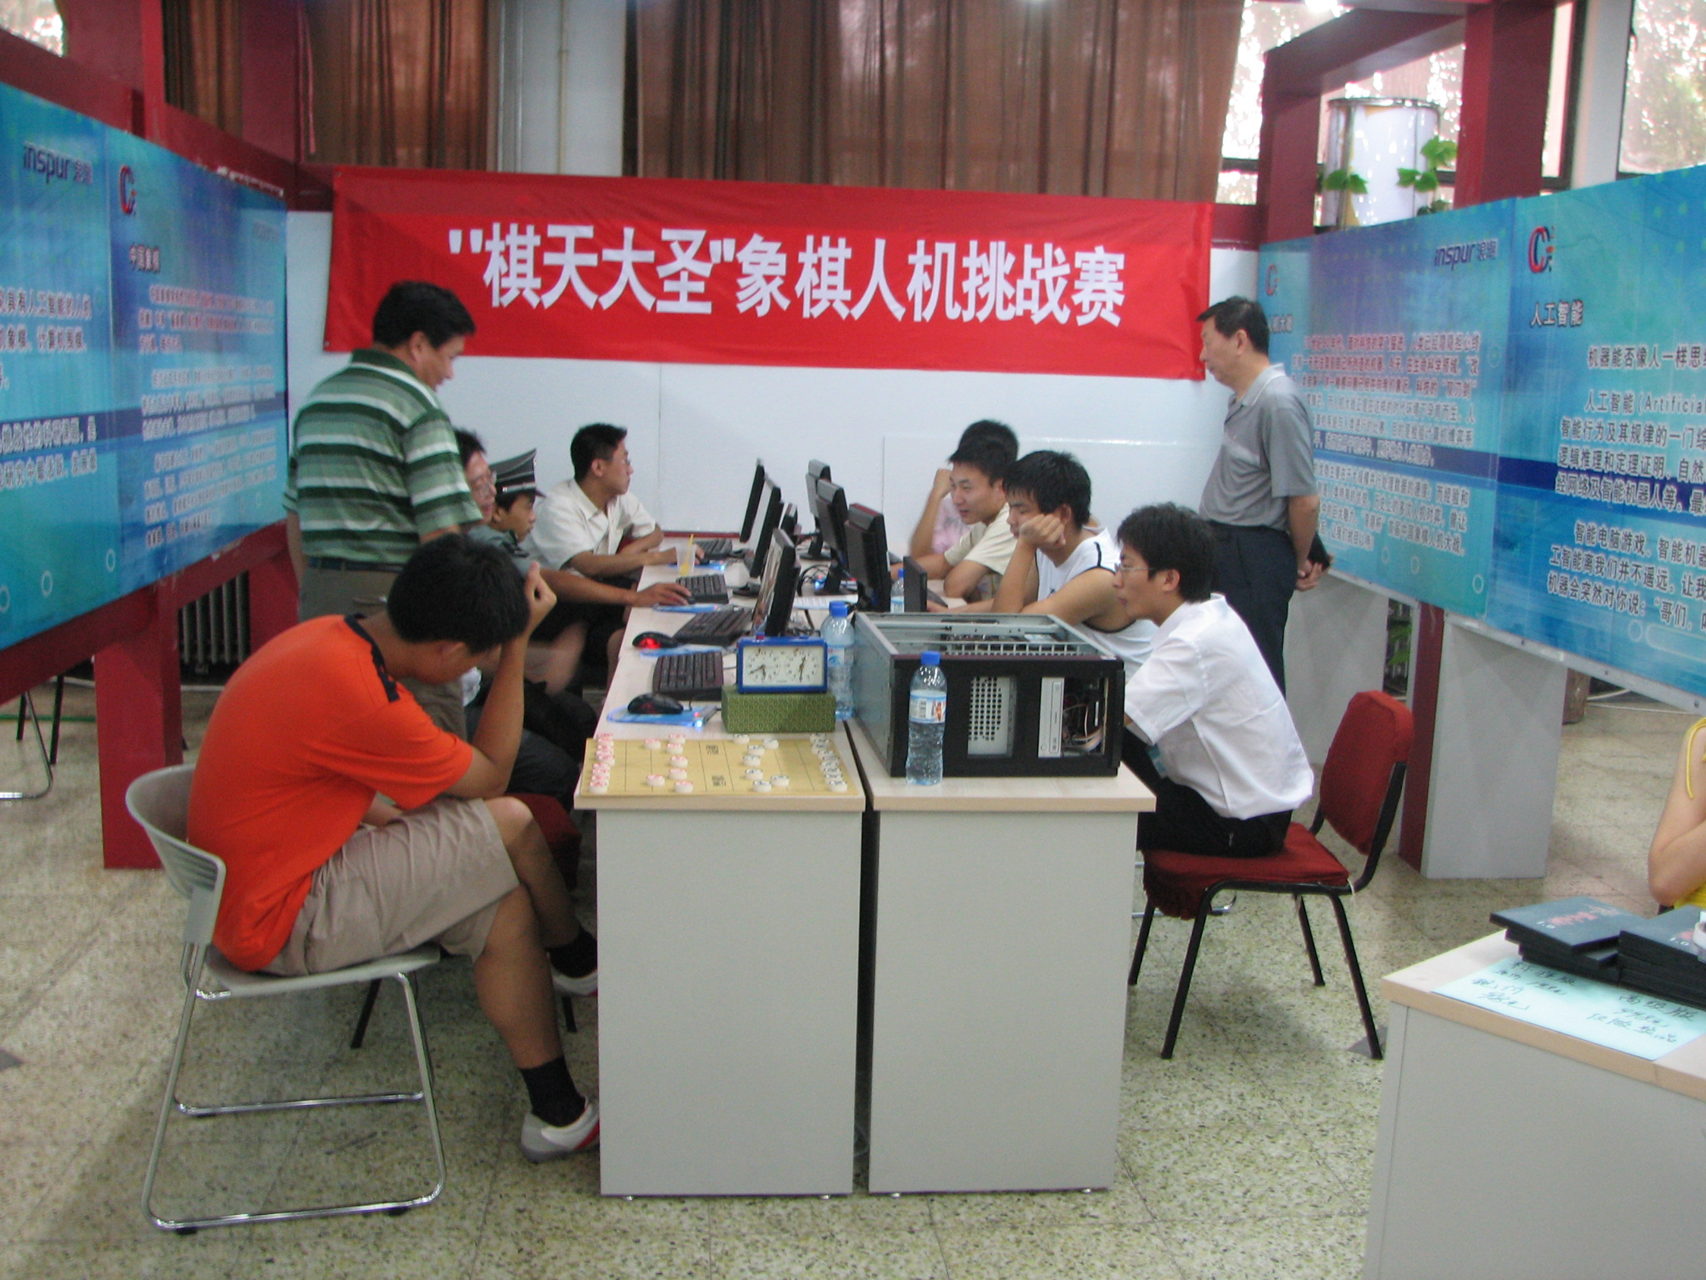
\includegraphics[width=0.45\textwidth]{xiangqitupian120104}\\
    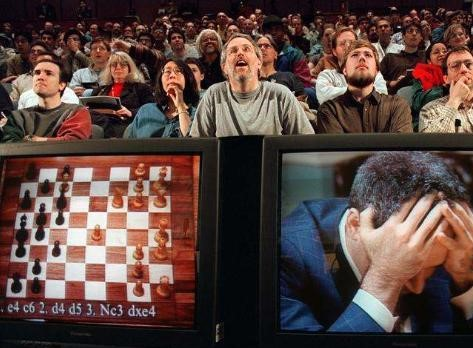
\includegraphics[width=0.465\textwidth]{fdanogetrwkxywvp!1200.jpeg}
    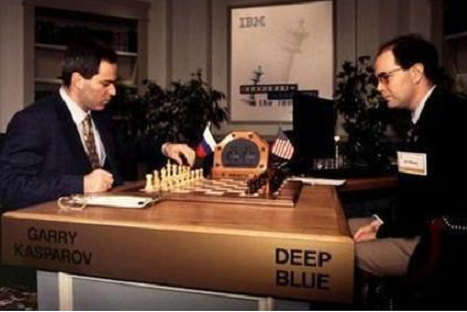
\includegraphics[width=0.513\textwidth]{b9xcph5lw6yp0cgb1200.png}
	\caption{象棋比赛,  “深蓝”击败Kasparov}
   \label{AI:Fig4}
\end{figure}
%%%%%%%%%%%%%%%%%%%%%%%%%%%%%%%%%%%%
\subsection{深度学习求解高维偏微分方程}
传统的求解PDE维数通常是二维或三维, 但在比如说金融学等领域, 通过数学建模构建出来的PDE的维数极其之高, 维数升高带来的“维数灾难”问题亟待解决.
深度学习的方法可以处理一般的高维抛物型方程, 用反向随机微分方程构造PDE, 并用神经网络近似未知解的梯度, 来求解高维的偏微分方程. 高维偏微分方程主要来自如下几个方面:
\begin{itemize}
\item 量子多体问题的薛定谔方程, 在这种情况下, PDE的维数大约是系统中电子或者量子(粒子)的三倍.
\item 用于给金融衍生品定价的Black-Scholes方程, 其中PDE的维数是所考虑的相关金融资产的数量.
\item 动态规划中的Hamilton-Jacobi-Bellman方程. 在具有多个代理的博弈论中, 维数随着代理的数量线性增加. 类似地, 在资源分配问题中, 维数随着设备和资源的数量线性增加.
\end{itemize}
这些问题的计算成本随维度呈指数增长!泛逼近定理保证深度学习网络能表示任意函数, 因此, 基本思路就是随机微分方程中某个梯度算子用神经网络来表示. \index{泛逼近定理}

\begin{example}
考虑一类半线性抛物型偏微分方程:
\begin{align}\label{DNNPDE20191218eq01}
\frac{\partial u}{\partial t}(t,  x)&+\frac{1}{2} \operatorname{Tr}\left(\sigma \sigma^{\mathrm{T}}(t,  x)\left(\mathrm{Hess}_{x} u\right)(t,  x)\right)+\nabla u(t,  x) \cdot \mu(t,  x)\notag\\
                               &+f\left(t,  x,  u(t,  x),  \sigma^{\mathrm{T}}(t,  x) \nabla u(t,  x)\right)=0.
\end{align}
且有指定的末端条件$u(T, x)=g(x)$, 这里的$x$是$d$维的, $\mu$是已知的向量值函数, $\sigma$是$d$维矩阵值函数, $f$是非线性函数.
\end{example}

我们感兴趣的是$t=0, x=\xi$的解. 让$X_t$是随机变量, 满足如下的方程
\begin{align}\label{DNNPDE20191218eq02}
  X_{t}=\xi+\int_{0}^{t} \mu\left(s,  X_{s}\right) d s+\int_{0}^{t} \sigma\left(s,  X_{s}\right) d W_{s}.
\end{align}
根据结果\cite{Han2018PNAS, Sirignano2018, Raissi2017}, 式\eqref{DNNPDE20191218eq01}的解具有如下形式:
\begin{align}\label{DNNPDE20191218eq03}
  u\left(t,  X_{t}\right)=u\left(0,  X_{0}\right)-\int_{0}^{t} f\left(s,  X_{s},  u\left(s,  X_{s}\right),  \sigma^{\mathrm{T}}\left(s,  X_{s}\right) \nabla u\left(s,  X_{s}\right)\right) d s\notag\\
                        \quad +\int_{0}^{t}\left[\nabla u\left(s,  X_{s}\right)\right]^{\mathrm{T}} \sigma\left(s,  X_{s}\right) d W_{s}.
\end{align}
我们对式\eqref{DNNPDE20191218eq02}和式\eqref{DNNPDE20191218eq03}两个式子用\uwave{欧拉格式}离散, 得到:
\begin{align}\label{DNNPDE20191218eq04}
  X_{t_{n+1}}-X_{t_{n}} \approx \mu\left(t_{n},  X_{t_{n}}\right) \Delta t_{n}+\sigma\left(t_{n},  X_{t_{n}}\right) \Delta W_{n}.
\end{align}

\href{https://blog.csdn.net/lusongno1/article/details/83867550}{想法}就是用其他格式离散化原始的方程, 比如说Milstein格式等.
接下来是关键的步骤, 就是在数值格式中, 用多层反馈神经网络去逼近$o(\nabla u)$项, 即:
\begin{align}\label{DNNPDE20191218eq07}
\sigma^{\mathrm{T}}\left(t_{n},  X_{t_{n}}\right) \nabla u\left(t_{n},  X_{t_{n}}\right)=\left(\sigma^{\mathrm{T}} \nabla u\right)\left(t_{n},  X_{t_{n}}\right) \approx\left(\sigma^{\mathrm{T}} \nabla u\right)\left(t_{n},  X_{t_{n}} | \theta_{n}\right).
\end{align}
注意到\label{DNNPDE20191218eq05}这里每一步都放进去一个神经网络, 最后整个堆叠成一个函数表达器. 这里边的$X_{t_{n}},  W_{t_{n}}$是变量. 我们可以用一般的深度学习方法来训练这个网络, 如随机梯度下降方法等.
还记得我们前面给了一个末端条件, 刚好可以用了定义损失函数.
\begin{align}\label{DNNPDE20191218eq08}
  l(\theta)=\mathbb{E}\left[\left|g\left(X_{t_{N}}\right)-\hat{u}\left(\left\{X_{t_{n}}\right\}_{0 \leq n \leq N}, \left\{W_{t_{n}}\right\}_{0 \leq n \leq N}\right)\right|^{2}\right],
\end{align}
其中$\theta_n$是神经网络的参数(权重系数), 上述方法称为深度BSDE方法.\index{深度BSDE方法}
%%%%%%%%%%%%%%%%%%%%%%%%%%%%%%%%%%%%%%%%%%%%%%%%%%%%%%%%%%%%%%
\begin{example}
(带违约风险的Black-Scholes方程)
 金融衍生品交易的一个关键问题就是确定适当而公平的价格. Black和Scholes说明了衍生品的价格$u$满足一个抛物型的PDE, 现在被称为Black-Scholes方程. Black-Scholes模型可以加以考虑实际市场中的几个重要因素, 包括可违约证券, 借贷利率高于贷款利率, 交易成本, 模型参数的不确定性等等. 这几个效应中的每一个都会在定价模型中产生非线性的贡献. 特别是, 信贷危机和持续的欧洲主权债务危机凸显了原始的Black-Scholes模型中忽略的最基本风险, 即违约风险.

理想情况下, 定价模型应考虑金融衍生品所依赖的整个底层证券, 从而产生了了高维非线性偏微分方程. 然而, 由于维数的诅咒, 现有的定价算法通常无法解决这些问题. 为了证明深度BSDE方法的有效性, 作者研究了一个具有违约风险的递归估值模型的特例.
我们考虑尚未发生违约的情况下, 100个标的资产的欧洲债权的价格是公平的. 当违约的情况发生时, 索赔的持有人仅收到当前值的分数倍, 设为$\delta\in [0, 1)$.
对于强度$Q$(当前值的递减函数), 可能风险由泊松过程的第一个跳跃时间建模得到, 换言之, 当声明的值低时, 风险变得更加可能. 可以通过以下方式对价值变化过程进行建模:
\begin{align}
  f\left(t,  x,  u(t,  x),  \sigma^{\mathrm{T}}(t,  x) \nabla u(t,  x)\right)=-(1-\delta) Q(u(t,  x)) u(t,  x)-R u(t,  x),
\end{align}
其中$R$是无风险资产的利率.  我们假设标的资产价格做几何布朗运动, 并选择强度函数$Q$为当前值的分段线性函数, 有三个区域($\mathrm{v_h}<\mathrm{v}_l,  \mathrm{\gamma_h}>\gamma_l)$), 函数形式如下:
\begin{align}
  Q(y)=1_{\left(-\infty,  v^{h}\right)}(y) \gamma^{h}+1_{\left[v^{l},  \infty\right)}(y) \gamma^{l}+1_{\left[v^{h,  v l}\right)}(y)\left[\frac{\left(\gamma^{h}-\gamma^{l}\right)}{\left(v^{h}-v^{l}\right)}\left(y-v^{h}\right)+\gamma^{h}\right],
\end{align}
那么, 在$[0, T]\times \mathbb R^{100}$上的非线性Black-Scholes方程就变为了:
\begin{align}
  \frac{\partial u}{\partial t}(t,  x)+\bar{\mu} x \cdot \nabla u(t,  x)+\frac{\bar{\sigma}^{2}}{2} \sum_{i=1}^{d}\left|x_{i}\right|^{2}
       \frac{\partial^{2} u}{\partial x_{i}^{2}}(t,  x)-(1-\delta) Q(u(t,  x)) u(t,  x)-R u(t,  x)=0.
\end{align}
设置如下参数, $T=1, \delta=2/3, R=0.02, \mu=0.02, \sigma=0.2, v_h=50, v_l=70, \gamma_h=0.2, \gamma_l=0.02$, 终止条件$g(x)=min\{x_1, x_2, ..., x_{100}\}$. 网络学习过程见图\ref{DNNBSDE1218Fig4}.
\end{example}
\begin{figure}[htbp]
	\centering
	\includegraphics[width=0.85\textwidth]{DNNBSDE1218.png}
	\caption{深度BSDE的结构}
   \label{DNNBSDE1218Fig4}
\end{figure}
%%%%%%%%%%%%%%%%%%%%%%%%%%%%%%%%%%%%
\subsection{自动定理证明}
自动定理证明的概念: 就是让计算机模拟人类证明定理的方法, 自动实现像人类证明定理那样的非数值符号演算过程. 它既是人工智能的一个重要研究领域, 又是人工智能的一种实用方法.
除数学定理外, 多非数学领域的任务如医疗诊断、难题求解等都可转化成定理证明问题.
%%%%%%%%%%%%%%%%%%%%%%%%%%%%%%%%%%%%
\begin{remark}
数学定理证明机械化的途径很多, “吴方法”是其中的代表. 对于初等平面几何, “吴方法”实质上就是“方程联立求证法”.
\begin{example}(方程联立求证法)
  我们需要求证一个几何“事实”(或断语): 三线“共点”. 看起来这是显而易见的事情, 但是, 使用计算机自动证明这一事实却并不容易.
\end{example}

$\bullet$ 吴方法的第一步: 实现“代数化”, 即建立坐标系, 把问题条件全部翻译成“代数方程式”(事项即“前提条件”), 然后, 把需要证明的事实也翻译成“代数方程式”(有待证明的事项). 吴方法的第二步: 方程联立求证.

$\bullet$ 把前提条件(方程组)与待证明的方程“联立求解”, 如果待证明的“方程”经过自动联立求解过程, 变为一个恒等式, 那么, 这个恒等式就表示“所有前提条件”满足待证的“结论”, 所以, 定理得到证明, 否则, 问题无解.

$\bullet$ 在国际学术界, “吴方法”独树一帜, 不随大流, 效率最高, 得到国际同仁赞扬与肯定. 经过多年人才积累, 在数学定理证明机械化研究领域, 研究业绩非凡, 国内”吴氏学派“最终形成.

$\bullet$ \href{http://www.mmrc.iss.ac.cn/}{中科院数学机械化重点实验室},  成员包括万哲先院士、陆汝钤院士、李邦河院士、张景中院士、林惠民院士等10多位实验室学术委员会成员.

$\bullet$ 吴文俊人工智能科学技术奖:  吴文俊是我国著名数学家、首届国家最高科学技术奖获得者. 吴文俊人工智能科学技术奖由中国人工智能学会发起设立, 设有成就奖、创新奖和进步奖, 每年评奖一次, 奖励在智能科学技术领域取得重大突破、作出卓著贡献的科技工作者和管理者. (转自科学网)

$\bullet$ 符号和代数计算方面最权威的国际会议——国际符号和代数计算会议(ISSAC).

$\bullet$  2019年是“吴文俊人工智能科学技术奖”的第九届.
\end{remark}

\begin{remark}
首届国家最高科学技术奖获得者、中国科学院院士、中国人工智能学会名誉理事长吴文俊先生命名, 依托社会力量设立的科学技术奖 . 由国家一级学会——中国人工智能学会发起主办, 被誉为“中国智能科学技术最高奖”, 至今已累计对314个单位及行业机构、291个创新成果和项目、973名学者及专家进行表彰.
\end{remark}

\begin{center}
\begin{minipage}{0.8\textwidth}
  第三届吴文俊人工智能科学技术奖于2013年10月29日在深圳揭晓.

  \ding{172} 中国科学院史忠植的“拓展知识工程核心理论, 创新分布智能理论基础, 构建智能科学理论体系”成果获吴文俊人工智能科学技术奖成就奖;

  \ding{173}大连理工大学李洪兴的“模糊系统的概率表示与空间四级倒立摆的控制”成果;

  \ding{174}北京航空航天大学段海滨的“群体智能及其应用”成果分别获创新奖一等奖;

  \ding{175}清华大学唐杰的“研究者社会网络搜索与挖掘系统”项目获进步奖一等奖.

  \ding{176}北京大学刘宏在面向服务机器人的视听感知与人体运动分析领域的创新工作;

  \ding{177}西安电子科技大学的公茂果在自然计算理论及其在SAR图像解译中的应用领域的创新工作分别获得创新奖二等奖.
\end{minipage}
\end{center}
%%%%%%%%%%%%%%%%%%%%%%%%%%%%%%%%%%%%
自动定理证明的主要方法:
\begin{itemize}
\item 自然演绎法: 其基本思想是依据推理规则, 从前提和公理中推出一些定理, 如果待证明的定理在恰在其中, 则定理得证. 这种方法的突出代表是纽厄尔等人研制的数学定理证明程序LT等.
\item 判定法: 其基本思想是对某一类问题找出一个统一的、可在计算机上实现的算法. 其突出代表是我国数学家吴文俊院士提出的证明初等几何定理的算法. 其基本思想是把几何问题代数化, 即先通过引入坐标把几何定理中的假设和求证部分用一组代数方程表达出来, 然后再利用代数几何中的代数簇.
\item 理论求解代数方程, 以证明定理的正确性.
\item 定理证明器: 是一种研究一切可判定问题的证明方法. 其典型代表是1965年鲁宾逊提出的归结原理.
\item 人机交互定理证明: 是一种通过人机交互方式来证明定理的方法. 它把计算机作为数学家的辅助工具, 用计算机来帮助人完成手工证明中难以完成的那些计算、推理、穷举等. 其典型代表是四色定理证明.
\end{itemize}
%%%%%%%%%%%%%%%%%%%%%%%%%%%%%%%%%%%%
\subsection{\textbf{国家安全领域}}
2019年3月, 全球安全研究中心劳伦斯利佛摩国家实验室(CGSR Lawrence Livermore National Laboratory)的扎卡里·戴维斯(Zachary Davis,  加州蒙特利海军研究生院的教授)高级研究员发布题为《战场上的人工智能》(《AI on the battlefield》)的文章.
文章中指出, 人工智能突如其来地闯入国家安全领域, 并被视为一种革命性技术, 与发现燃料、电力或核武器不相上下. 人工智能技术在一定程度上对美国产生了变革效应(例如, 在科学和社交媒体中), 在一定程度上这是由美国潜在对手驱动的. 俄罗斯总统普京宣称, 统治人工智能的国家将是世界的统治者.
\begin{figure}[htbp]
	\centering
	\includegraphics[width=0.55\textwidth]{934ceac90e21bd317dae.jpeg}
	\caption{未来战争}
   \label{AI:201912020Fig4}
\end{figure}
%%%%%%%%%%%%%%%%%%%%%%%%%%%%%%%%%%%%
%%%%%%%%%%%%%%%%%%%%%%%%%%%%%%%%%%%%
\subsection{\textbf{机器人}}
Spot 机器狗已经参与了“至少两次”实际执法活动.
\begin{figure}[H]
	\centering
	\includegraphics[width=0.445\textwidth]{A87bf40ad1cb80.png}
	\includegraphics[width=0.453\textwidth]{Boston1233465768.PNG}
	\caption{波士顿机械狗}
   \label{AI:7bf40ad1cb80Fig4}
\end{figure}

2020年2月13日, 伊朗推出迄今为止最先进的类人机器人Surena 4(又称Surena IV, 图\ref{SurenaIVFig2}).
Surena 4新机器人是对以前设计的重大改进. 突出的功能是它能模仿人的姿势, 抓住水瓶并将其名字写在白板上, Surena 4还能自己步行走出学校大门, 抓或者捧较大的球形物体.
%\begin{figure}[htbp]
%\begin{center}
%\begin{figure}[htbp]
%\includegraphics[width=0.6\textwidth]{SurenaIV.gif}
%\caption{图灵测试}
%\label{AI:turingFig1}
%\end{figure}
%\end{center}
%\caption{Surena 4运动图}
%\label{SurenaIVFig2}
%\end{figure}
%%%%%%%%%%%%%%%%%%%%%%%%%%%%%%%%%%%%%%%%%
\begin{figure}[H]
\centering
\animategraphics[width=0.86\textwidth,autoplay,controls]{2}{SurenaIV}{1}{10}
\caption{Surena 4运动图}
\label{SurenaIVFig2}
\end{figure}
Surena 由德黑兰大学机械工程学教授尤塞菲·科马博士在50多名研究人员的领导下在CAST(先进系统和技术中心)开发.
Surena机器人的第一代(SURENA I, 2008年)只有8个自由度(DoF), 第二代(SURENA II, 2010年)有22个自由度, 行走速度为每秒0.03米.
与拥有31 DoF的第三代(SURENA III, 2015)相比, 新型第四代机器人(Surena IV, 2019)具有43 DoF和更高的手部灵活性, 使其能够抓握具有不同形状的不同物体.
Surena 4高1.7米, 重68公斤;它比Surena III(98公斤高和1.9米高)更轻巧, 更小, 这归功于其基于拓扑优化的更好的结构设计, 紧凑的定制执行器设计以及SLA 3D打印技术.

在新一代Surena 4中, 通过利用FPGA板, 控制环路频率已提高到200 Hz, 从而可以实现在线控制器和估计器. 通过机器人操作系统(ROS), 状态监控, 算法的实时实现以及多个程序的同时运行变得非常简单.
Surena 4具有面部检测和计数, 物体检测和位置测量, 活动检测, 语音识别和语音合成的能力, 从而实现了更好的语音用户界面. 通过结合AI能力和全身运动计划, 实现了在线抓握, 面部和物体跟随以及动作模仿.
Surena 4可以以0.7公里/小时的速度连续行走. 它可以通过其底部的新型接触传感器在不平坦的地形上行走.
CAST装备了在线接触控制器, 可以在踩踏过程中调节脚的角度和位置.
用于模拟机器人的运动并评估不同的场景(凉亭和动物群), 包括侧向行走, 向后行走, 转身和推举恢复).
%%%%%%%%%%%%%%%%%%%%%%%%%%%%%%%%%%%%
\subsection{\textbf{机械臂}}

\begin{figure}[H]
	\centering
	\includegraphics[width=0.35\textwidth]{b151f8198618e3f6.jpg}
	\includegraphics[width=0.35\textwidth]{267f9e2f0708ff82.jpg}
	\caption{堆垛和切割钢铁建材}
   \label{AI:7bf40ad1cb80Fig4}
\end{figure}
%%%%%%%%%%%%%%%%%%%%%%%%%%%%%%%%%%%
\textbf{智能软体机器人}
%%%%%%%%%%%%%%%%%%%%%%%%%%%%%%%%%%%%%%%%%%
\begin{figure}[H]
\centering
\includegraphics[width=0.45\textwidth]{softissuerobot.jpg}
\caption{DNA软体机器的设计原理图}
\label{softissuerobot}
\end{figure}
%%%%%%%%%%%%%%%%%%%%%%%%%%%%%%%%%%%%
\subsection{闲鱼垃圾评论过滤系统}
闲鱼垃圾评论过滤系统(训练并推断 11 亿节点的图)用了最前沿的图卷积神经网络. 这项研究获得了 ACM CIKM 2019 最佳应用论文奖, 说明图卷积在传统任务中的强大潜力.
垃圾信息过滤表面上它只是一个最简单的二分类问题, 对于闲鱼这种开放性评论机制, 评论的维度及角度非常多种多样, 再来筛选垃圾信息就非常困难了.
常规做法是通过关键字判断垃圾信息, 也有采用朴素贝叶斯等浅层模型, 还有 TextCNN 等深度神经网络, 很多算法都是从文本层面判断评论是不是垃圾评论.
很多时候, 光使用文本是不够的, 闲鱼的场景的灰产和模型一直在对抗, 垃圾评论变异得很快.
闲鱼需要结合一些难以变异的特征判断评论是不是垃圾评论, 包括发送这条评论的用户信息、接收这条评论的商品特征, 甚至是发送这条信息的用户, 他的其它评论行为; 以及与它类似的文本都有什么特征.
要利用这些多模态信息与复杂的图结构信息, 就需要更强大的前沿模型——\textbf{图卷积神经网络}.

目前评论过滤系统已经部署到了闲鱼使用环境中, 每天能处理百万级的闲鱼评论, 并在其他强有力的深度学习模型基础上, 额外筛选出一千多条非常隐秘的垃圾评论.
阿里研究者表示: 基于图卷积的垃圾信息筛选是一种非常通用的思想, 它的应用范围远不止垃圾评论过滤, 淘宝信息的知识产权保护、淘宝商品管控和用户恶意评价等方面都可以采用.
图神经网络还是非常有前景的, 加上图神经网络可以利用复杂图数据的结构信息和多模态属性信息, 业务场景非常广.

闲鱼是国内最大的二手交易平台, 我们可以浏览卖家发布的各种商品, 并根据描述与评论选择合适的物品. 然而, 这个每天交易超过 20 万商品的平台, 却会受到垃圾评论的困扰.
这主要是因为它与淘宝不一样, 淘宝只有买过商品才能评价, 但是对于闲鱼, 评论充当着买卖双方的沟通工具, 很多评论行为发生在购买之前.
正式这种提前沟通与议价的机制, 为垃圾评论提供了合适的平台. 想象一下, 如果灰产用户在许多受关注的商品中留言自己的广告, 这样岂不是非常「划算」?
为此, 阿里的研究者一直与垃圾评论做着对抗, 垃圾评论越来越「隐秘」, 而判别算法也越来越「聪明」.
我们先看看广告评论怎样越来越隐秘:
换个说法: 使用不同的方式表达相同的意思, 例如「拨打电话获得更多兼职信息」和「闲余时间挣点钱?联系我」, 这两者都引导我们关注相同的兼职广告.
关键字替换: 使用少见的中文字符、笔误, 甚至表情符号替换关键字, 例如「加我的 VX/V/WX」都表示加我的微信.
垃圾评论发布者的这些小技巧很容易欺骗一般的机器学习系统, 与此同时, 如果发布者发现这些方法不太管用, 他们又会挖掘一些新技巧. 因此这样总是防不胜防, 已经部署的防控算法的效果也会逐步降低. 所以如果是一个好的垃圾评论过滤系统, 它首先要捕捉到现有的各种模式, 与此同时还应该降低对抗行为对系统的影响.
解决思路是什么?
解决垃圾信息过滤的核心思想在于上下文, 我们只有把文本信息放入对应的环境, 才能准确判断它到底是不是垃圾评论.
阿里研究者定义了两种上下文, 即局部上下文和全局上下文. 其中局部上下文包含发这条评论的买家特征及行为和这条评论对应的商品特征等信息,
而全局上下文表示当前评论在全部评论中的扮演的角色 ( \href{https://arxiv.org/abs/1908.10679}{Spam Review Detection with Graph Convolutional Networks}).

以两种上下文信息为出发点, 研究者设计了名为 GCN-based Anti-Spam System(GAS) 的垃圾评论过滤系统. 如下所示为 GAS 的整体概览, 其中模型会从左侧图抽取出表示商品、用户和评论的信息, 从右侧抽取出类似评论表示的意义. 最后结合这些信息进行分类, 模型就能很好地识别垃圾信息了.

GAS 会使用两个图来引入不同的上下文的信息. 闲鱼 Graph 是一个异构图, 它引入局部上下文信息, 另一个是同构图 Comment Graph, 它引入了全局上下文信息.
在这两个图上, 研究者分别运行不同的图卷积算法, 并最终融合两个图模型的上下文信息, 从而共同判断一个评论是不是有问题.
这项研究比较重要的地方在于, 研究者基于他们对业务的理解, 所设计的图网络结构能够完成两种上下文信息的抽取, 从而真正提升业务场景的效果.
研究者说: 「这是我们论文最主要的贡献之一, 我们会把传统的文本分类的问题抽象成异构图上的边分类问题, 把图卷积算法和文本分类做一个很好的结合.
不光是在做垃圾检测的过程当中, 阿里在研究与业务中都会遇到很多特定问题.
很多情况下, 我们很难从学术界直接套用一些好的方法, 因此经常要把成熟或新颖的算法匹配到业务上, 这些匹配很可能做出一些新的贡献.

图卷积是非常神奇的一个模型, 它能处理图这种结构化的数据. 要理解图卷积, 需要包括傅立叶变换、拉普拉斯算子等数学基础.
自 ICLR 2017 Kipf 的文章发表以来, 图卷积才逐渐受到更多的关注, 该论文从频域的角度将 CNN 转移到了 Graph, 并推导出了非常简单优雅的形式.
研究者又从空域的角度提出了 GraphSAGE, 它利用直观的节点采样与特征聚合高效地生成节点向量,
后面还有 Bengio 组的 GAT 与 MIT 的 jumping knowledge net.
\href{https://arxiv.org/abs/1609.02907}{图卷积开山之作:Semi-Supervised Classification with GCN}

除了模型与研究上的创新, 阿里研究者在工程上也做了很多努力. 因为对于闲鱼 Graph 这种超过 10亿商品与 1亿用户的节点量, 要做训练和推断都是比较复杂的.
目前该系统已经基于 TensorFlow 分布式框架部署在服务端, 最开始没有成熟的大规模图框架, 基于 TensorFlow 的参数服务器框架,  将图和特征放到参数服务器上, 而后最核心的采样与卷积操作都是从上面获取数据, 整个就是一个分布式系统.
当然后来阿里内部研发了大规模图框架 AliGraph, 研究团队将系统迁移到 AliGraph 后进一步提升了效率.
%%%%%%%%%%%%%%%%%%%%%%%%%%%%%%%%%%%%
\subsection{PCB产业}
PCB已经发展到全新阶段, 诸如高密度互连(HDI)PCB, IC基板(ICS)等全新技术引入, 使得整个生产过程从手动变成了全自动化.
随着制造技术的进一步发展, 工艺变得越来越复杂, 缺陷检查越来越重要也越来越难, 这些致命缺陷可能会导致整个PCB板的报废. 对于PCB制造业来说, 利用人工智能(AI)并优化生产工艺以及最终优化整个PCB制造流程的机会正在涌现.

PCB制造通常依赖多年积累知识的专家, 这些专家非常了解和理解制造过程的每个步骤, 他们了解如何利用他们的知识来优化生产和提高产量.
人为的限制(包括误操作和疲劳)阻碍了效率增长, 操作员的错误或对PCB缺陷的错误识别(“错误警报”)可能会由于过度处理而影响良率, 甚至会损害PCB本身.
通过将AI集成到制造过程中(图\ref{AIPCB811Fig4}), 机器可以通过接管某些“学习的”任务来增加价值, 而人类专家则继续承担更复杂的任务, 这些任务需要在优化和“培训”的同时进行思考和互动人工智能系统.
人与人工智能的结合提高了整体效率和运营, 是AI系统的最大机会.

PCB发展的最终趋势是拥有完全集成Industry 4.0系统的工厂, 该系统在全球和制造系统级别采用AI技术. “全局”级别包括工厂中的所有系统, 而不仅仅是单个制造系统.
工业4.0提供了自动化和数据交换基础结构, 可实现实时生产分析, 双向通信和数据共享, 可追溯性以及按需数据分析.
在任何特定的工厂内, AI都可以使用从各种制造系统和机器获取的数据来改进流程, 这些数据是通过工业4.0机制(例如可追溯性, 双向通信)收集的.
工厂之所以受益, 是因为AI分析了大量的系统范围数据以优化工厂设置参数并实现最高水平的生产率和良率.
人工智能分析和自我学习正在进行中, 并通过人工神经网络进行. 几年之内, 它将消除人工操作人员的干预, 并导致建立全自动工厂.
%%%%%%%%%%%%%%%%%%%%%%%%%%%%%%%%%%%
\begin{figure}[H]
	\centering
	\includegraphics[width=0.75\textwidth]{AIPCB811.png}
	\caption{AI可以帮助PCB工厂提高质量}
   \label{AIPCB811Fig4}
\end{figure}
%%%%%%%%%%%%%%%%%%%%%%%%%%%%%%%%%%%

这种新的PCB制造模型要求将所有工厂系统完全连接以及AI作为监视和决策机制. 当前, 存在专有和技术挑战, 这些问题限制了PCB工厂的完全自动化, 但AI已尽可能地添加到单个系统中, 例如自动光学检查(AOI)解决方案. 将生产设施移向全球AI模型的优势包括, 可以更可靠地通知PCB缺陷——“真实缺陷”, 并具有反馈机制, 该反馈环可以识别问题的根源, 然后自动修改工厂流程以消除相关问题缺陷.

AI包括机器学习和深度学习, 将使PCB工厂朝着完全自动化的目标迈进. 机器学习使用的算法使计算机能够使用数据及其已经经历并从中学习的示例来改进任务的性能, 而无需对其进行明确的编程. 就PCB制造而言, 机器学习可提高产量, 改善制造操作和工艺流程并减少人工操作, 同时有助于推动对工厂资产, 库存和供应链的更有效处理.

深度学习将AI提升到一个更加复杂的水平, 这在全球工厂系统水平上是有益的. 深度学习的灵感来自人脑神经元, 多层人工神经网络进行学习, 理解和推断的能力. 在PCB工厂中, 软件系统可以有效地收集的数据, 并利用模式和上下文的复杂表示中学习, 然后, 学习将形成PCB制造中自动过程改进的基础.
机器学习和深度学习的实施为PCB制造商提供了超越人类理解的能力; 人工智能系统通过在人们不愿探索的地方进行更深入的挖掘来发现新的优化机会. AI专家系统非常高效, 通过使用更多更复杂的参数在全球范围内监控工厂系统, 减少了所需的人工专家数量, 并提高了效率和最佳实践.
%%%%%%%%%%%%%%%%%%%%%%%%%%%%%%%%%%%%
\subsection{百度飞桨: 开源开放的产业级深度学习平台}
深度学习框架上承应用下接芯片, 是智能时代的操作系统. 在关键技术上, 中国必须通过自主研发掌握主动权. \href{https://www.paddlepaddle.org.cn/}{百度飞桨}是中国首个也是目前国内唯一开源开放、功能完备的产业级深度学习平台, 在今年也取得了长足的进步, 如今已经具备开发便捷的产业级深度学习框架、超大规模深度学习模型训练技术、多端多平台部署的高性能推理引擎、开源开放覆盖多领域的产业级模型库四大领先技术. 通过有效降低深度学习技术应用门槛, 飞桨让开发者和企业避免重复“造轮子”, 更快速、便捷地开发AI应用. 目前, 飞桨已经累计服务150多万开发者, 定制化训练平台上企业用户超过6.5万, 发布了16.9万个模型, 已广泛应用于工业、农业、服务业等各个行业, 实现“遍地开花”. 据IDC报告显示, 在国内深度学习平台市场中, 百度与谷歌、Facebook三强鼎立, 已经占据了国内超过七成的市场份额, 其中百度的市场份额在过去半年里仍在迅猛增长, 展现出领军者的不俗实力.
%%%%%%%%%%%%%%%%%%%%%%%%%%%%%%%%%%%
\begin{figure}[H]
	\centering
	\includegraphics[width=0.65\textwidth]{BaiduPeddle20191217.png}
	\caption{开源开放的产业级深度学习平台——百度飞桨}
   \label{BaiduPeddle20191217}
\end{figure}
%%%%%%%%%%%%%%%%%%%%%%%%%%%%%%%%%%%

CPU版本安装: pip install -i https://mirror.baidu.com/pypi/simple paddlepaddle, Pycharm下的百度飞桨训练uci\_housing数据集的示例见图\ref{BAIDUAIpaddletest202013001}.
%%%%%%%%%%%%%%%%%%%%%%%%%%%%%%%%%%%
\begin{figure}[H]
	\centering
	\includegraphics[width=0.65\textwidth]{BAIDUAIpaddletest202013001.PNG}
	\caption{Pycharm下的百度飞桨示例(uci\_housing)}
   \label{BAIDUAIpaddletest202013001}
\end{figure}
%%%%%%%%%%%%%%%%%%%%%%%%%%%%%%%%%%%
%%%%%%%%%%%%%%%%%%%%%%%%%%%%%%%%%%%%
\subsection{计算机视觉的语义分割}
滴滴地图事业部和加州大学伯克利分校的研究员提出一种新的多源领域自适应模型, 对多个不同源域的有标注合成数据和目标域的无标注真实数据进行联合学习, 显著提高了图像语义分割的性能. 据悉, 这是多源领域自适应第一次应用在语义分割任务上. 相关研究以「Multi-source Domain Adaptation for Semantic Segmentation」(基于多源领域自适应的语义分割)为题发表在神经计算和机器学习领域的顶级会议—第 33 届神经信息处理系统大会(NeurIPS 2019)上.
论文\href{https://arxiv.org/abs/1910.12181}{Multi-source Domain Adaptation for Semantic Segmentation},  \href{https://github.com/Luodian/MADAN}{论文代码}

卷积神经网络(convolutional neural networks,  CNNs), 人们提出了多种端到端的语义分割方法. 虽然这些方法取得了良好的效果, 但也存在一定的局限性. 一方面, 训练这些方法需要使用像素级标注的大规模数据, 这是非常昂贵和耗时的. 例如, 在 Cityscapes 数据集中标注每幅图像大约需要 90 分钟. 另一方面, 由于存在领域偏移(domain shift)或数据集偏差(dataset bias), 他们不能很好地将所学知识迁移到新的域或数据集. 为了避免数据收集和标注的成本, 图形学和仿真软件的发展使得研究者们可以使用 CARLA 和 GTA-V 等模拟器所生产的无限量合成标注数据.
为了减少不同领域之间的差距, 研究者们提出了领域自适应(domain adaptation,  DA)或知识迁移技术(knowledge transfer techniques), 并进行了理论分析和算法设计. 语义分割的领域自适应算法在自动驾驶等领域具有重要的作用. 现有的工作主要关注于单个源域的场景, 很难处理实际中具有不同分布的多个源域的情况. 在这篇论文中, 研究者们研究了基于多源领域自适应的语义分割.
%%%%%%%%%%%%%%%%%%%%%%%%%%%%%%%%%%%
\begin{figure}[H]
	\centering
	\includegraphics[width=0.85\textwidth]{Simetics8dbce236d19619.jpeg}
	\caption{语义分割}
   \label{Simetics8dbce236d19619}
\end{figure}
%%%%%%%%%%%%%%%%%%%%%%%%%%%%%%%%%%%
\textbf{现有自适应方法在图像分割上的挑战}

除了传统的有标注源域上的任务损失外, 深度无监督领域自适应(UDA)方法通常还会训练其他损失函数来处理领域偏移, 如差异损失(discrepancy loss)[2]、对抗损失\footnote{\href{https://colab.research.google.com/github/tensorflow/hub/blob/master/examples/colab/biggan_generation_with_tf_hub.ipynb}{BigGAN: Large Scale GAN Training for High Fidelity Natural Image Synthesis} \label{GANnote2020031201}}(adversarial loss)\cite{ZhuPark20178237506}、重构损失(reconstruction loss)\cite{GoodfellowGAN2014}等.
目前语义分割任务上从合成数据到真实场景的领域自适应方法都集中在单数据源设置上, 没有考虑从多个不同分布的数据源收集数据这一更实际的场景. 简单地将不同的源组合成一个源并直接使用单一源 DA 不会有很好的效果, 因为来自不同源域的图像在学习过程中可能会相互干扰. 早期对多源 DA(multi-source DA,  MDA)的研究使用了浅层模型.
近年来, 人们提出了一些多源深度 UDA 方法, 这些方法主要针对图像分类 \cite{Ghifary2015}. 由于以下原因, 直接将这些 MDA 方法从分类扩展到分割可能不会有很好的效果. (1) 分割是一个结构化的预测任务, 其决策函数比分类更复杂, 因为它必须在指数大的标签空间中解析预测 \cite{Zhang2017}. (2) 目前的 MDA 方法主要关注特征级对齐, 只对高层次的信息进行对齐. 这对于粗粒度的分类任务来说可能足够了, 但是对于细粒度的语义分割来说显然是不够的, 因为分割是像素级的预测. (3) 这些 MDA 方法只将每个源域和目标域对齐. 虽然不同的源域被匹配到目标域, 但在不同的源域之间可能存在显著的不一致.

多源对抗域聚合网络算法基于对抗生成式网络(GAN)\cite{GoodfellowGAN2014} 和循环对抗生成式网络(CycleGAN)\cite{ZhuPark20178237506}, 提出了一种新的端到端的多源对抗域聚合网络(Multi-source Adversarial Domain Aggregation Network,  MADAN), 框架如图\ref{MADANe38db3d1e}所示. MADAN 主要包括三个模块: (1) 动态对抗图像生成模块(Dynamic Adversarial Image Generation), (2) 对抗域聚合模块(Adversarial Domain Aggregation), (3) 分割特征语义对齐模块(Feature Aligned Semantic Segmentation).
%%%%%%%%%%%%%%%%%%%%%%%%%%%%%%%%%%%
\begin{figure}[H]
	\centering
	\includegraphics[width=0.65\textwidth]{MADANe38db3d1e.jpeg}
	\caption{MADAN 框架图}
   \label{MADANe38db3d1e}
\end{figure}
%%%%%%%%%%%%%%%%%%%%%%%%%%%%%%%%%%%
首先, 对于每个源域, 文章使用\href{https://blog.csdn.net/dugudaibo/article/details/82903233}{循环对抗生成式网络}(CycleGAN)\cite{Long2015CVPR} 生成一个动态保持语义并且具有像素级一致性的自适应域;
其次, 文章提出了子域聚合判别器(Sub-domain Aggregation Discriminator)和跨域循环判别器(Cross-domain Cycle Discriminator), 以使不同的自适应域更紧密地聚合; 最后, 在训练分割网络的同时, 对聚合域和目标域进行特征层面的对齐.
通过 MADAN, 不同的适应域可以更好地聚合为一个更统一的域. 基于聚合域对分割模型进行训练, 能够更好地提升分割模型在目标域上的表现.
%%%%%%%%%%%%%%%%%%%%%%%%%%%%%%%%%%%%
\paragraph{智能决策}
将人工智能纳入工作流程. 对于只依赖结构化数据的常规决策, 人工智能不受认知偏见的影响. 人工智能可以被训练为在人群中找到特殊——因为人类可能会因感情而产生偏见, 而人工智能却不会.
人工智能更适合处理非线性关系, 不管是指数关系、幂律关系、几何级数关系、二项式分布关系还是其他关系. 这些关系计算量庞大, 远远超出我们人类可以处理的范围.

人工智能工作流可以更好地利用数据中包含的信息, 并且在其决策中体现一致性并保持和观. 它可以更好地确定哪种广告创意最有效, 如何设定最佳的库存水平, 或者进行哪些金融投资.
%%%%%%%%%%%%%%%%%%%%%%%%%%%%%%%%%%%%
\subsection{威胁检测和预防}
网络安全威是当今任何组织面临的最大威胁, 系统、数据、云技术、应用程序、设备和分布式终端的激剧增加, 使得互联网面临越来越多的安全威胁, 安全网络也是5G和大数据技术的一个应用前提.
这意味着组织必须比以往任何时候都更加努力地工作, 以保护他们的资产和客户. 其实这已经超出了自动化对策的范围, 它现在要求信息安全专业人员积极主动地检测, 以先发制人地避免或阻止威胁.

如今的安全软件使用机器学习、深度学习、机器推理和一系列相关技术来审查大量数据, 其目的是加速对正常与异常的理解, 以检测恶意行为和实体.
到2022年, 全球信息安全支出预计将达到1700亿美元, 网络安全行业正在关注创新和效率, 更具弹性的机制和工具. 由于技术的进步, 信息安全中有四个主要的AI和机器学习场景, 下面我就来为大家一一讲解.
\begin{itemize}
\item \textbf{网络威胁分析}

如今的企业将越来越多的业务数字化, 他们会更新旧数据并开发内部(通常是混合)网络. 这些庞大的网络拓扑不仅复杂, 而且还需要大量的网络安全资源来管理所有通信、事务、连接、应用程序和策略.
如果企业规模很大, 则数字化不仅意味着巨大的投资, 而且还有数据被盗的风险. 人工智能在网络安全方面的应用, 完全可以应对这一挑战. 值得注意的是, 网络安全中的人工智能会监控所有传入和传出的网络流量, 以挖掘可疑活动并对威胁类型进行分类.

\item \textbf{恶意软件检测}

恶意软件是有攻击性的不断发展的代码或软件类别的总称, 尽管恶意软件检测已经存在多年了, 通常将可疑代码与基于签名的系统相匹配, 但机器学习现在正转向推理技术.
网络安全领域的人工智能在分析大量数据、事件类型、来源和结果时, 会在恶意文件被打开之前检测到恶意软件的存在. 它还可以识别恶意软件的类型, 因为恶意软件会随着其他技术的进步而不断发展, 比如恶意木马、僵尸网络、恶意广告、勒索软件等实例.
迄今为止, 深度学习和人工智能已经帮助各种安全应用程序从恶意软件和良性应用程序中获得的数以千万计的样本, 这样, 后期的检索就可以专门设置一个算法, 进行高效的检索, 这些都离不开精确标记的数据库.

\item \textbf{扩大安全分析的范围}

网络安全领域的人工智能最擅长发现潜在的威胁媒介, 不过是否算是真正的威胁, 还得依靠人类, 这意味着人类仍然是控制、解释和判断威胁的终结者. 只能说, 机器学习让人类变得更加强大了, 这主要体现在两个方面:

(1) 人工智能使重复的任务自动化, 例如, 它会对低风险警报或繁琐的数据任务进行分类, 以便让分析师有时间进行更高价值或战略决策.

(2) 机器学习负责低层次的威胁情报的数据整理和分析, 这样人类分析师就可以从基本的数据收集工作中解脱出来, 分析更有价值的信息, 以进行更高价值的战略决策.

实际的测试表明, 理想的网络安全性能或准确性往往是人类和人工智能的结合成果, 而不是单独进行判断. 安全工具的增强在未来几年对安全团队来说可能是必不可少的. 事实上, 市场上的一些技术已经支持UI工具, 使网络专家能够合并威胁类型来重新训练机器学习模型, 并根据问题配置特定的修复程序.

\item \textbf{基于人工智能的反向攻击}

任何技术的正反两面的发展趋势都是同步的, 企业必须训练机器学习算法, 以识别其他基于机器学习算法发起的攻击.
\begin{example}
有研究人员就发现黑客使用机器学习来识别企业网络中的薄弱环节. 他们使用此信息通过网络钓鱼, 间谍软件或分布式拒绝服务攻击将目标定为攻击入口点.
甚至已经有攻击者开发出了智能恶意软件, 它们还有另一个更可怕的称呼——人工黑客(artificial hackers), 以针对受害者的具体情况进行个性化攻击. 基于人工智能的攻击展示了人工智能的优势(快速可扩展性、行为分析和个性化)不仅安全人员看得到, 攻击者也看得到.
上述四个应用场景, 只是人工智能在网络安全领域众多应用中的一小部分. 不过要注意的是, 机器学习并不是万灵丹, 它只是人类的一个辅助工具. 传统的基于签名的检测方法的缺点, 机器学习中也存在.
同时, 它可以降低成本. 人工智能的价值在于做出比人类所能做得更好的决定, 这也就提高了效率, 为企业新的形态作出演变.
\end{example}
\end{itemize}
%%%%%%%%%%%%%%%%%%%%%%%%%%%%%%%%%%%%
\paragraph{智能网络}
\begin{Verbatim}
研究智能网络的意义

(1) 因特网在为人类提供了方便快捷的信息交换手段, 但基于因特网的万维网(WWW)
    却是一个杂乱无章、真假不分的信息海洋, 它不区分问题领域, 不考虑用户
    类型, 不关心个人兴趣, 不过滤信息内容.

(2) 传统的搜索引擎在给人们提供方便的同时, 大量的信息冗余也给人们带来了不少
   烦恼. 因此, 利用人工智能技术实现智能网络具有极大的理论意义和实际价值.

智能网络的两个重研究内容

(1) 智能搜索引擎是一种能够为用户提供相关度排序、角色登记、兴趣识别、
    内容的语义理解、智能化信息过滤和推送等人性化服务的搜索引擎.

(2) 智能网格是一种与物理结构和物理分布无关的网络环境, 它能够实现各种资源的
    充分共享, 能够为不同用户提供个性化的网服务. 可以形象地把智能网格比作一
    个超级大脑, 其中的各种计算资源、存储资源、通信资源、软件资源、信息资源、
    知识资源等, 都像大脑的神经元细胞一样能够相互作用、传导和传递, 实现资源
    的共享、融合和新生.
\end{Verbatim}
%%%%%%%%%%%%%%%%%%%%%%%%%%%%%%%%%%%%
\paragraph{微盟删库危机事件}
2020年3月1日, 微盟(SEHK:02013)官方发布公开信, 称在腾讯云团队协助下, 被删数据已全面找回, 同时公司将准备1.5亿元人民币赔付拨备金进行赔偿.
对于一家日均流水从三千元做到四万元的社区电商平台商户, 自备的ERP系统存有库存管理与订单管理数据, 波及到的仅有依靠微盟平台的会员系统与积分系统, 更严重的影响是用户信息的丢失.
该商户甚至因没有用户信息, “钱都在我手里, 但因为客户数据的丢失, 我都不知道该给谁发多少钱. ”
目前导致商铺线上全部崩溃, 无法经营, 对经营产生重大影响.
未来将会面临多方困难, 包括修复时间不可控, 运营成本上升, 客户及商家将考虑转移到其他平台, 面临更多或巨额赔偿, 流失潜在客户给竞争对手. 报告预期上述困难将给微盟带来长期负面影响.
%%%%%%%%%%%%%%%%%%%%%%%%%%%%%%%%%%%%%%%%%%%%%%%%%%%%%%%%%%%%%%%%%%%%%%%%%%%%%%%
\subsection{人工智能案例}
\begin{example}
  飞桨做的无人驾驶智能车: 吴东昱, 北京钢铁侠科技深度学习算法工程师, 主要研究深度学习、无人驾驶等.
\end{example}
%%%%%%%%%%%%%%%%%%%%%%%%%%%%%%%%%%%%%%%%%%%%%%%%%%%%%%%%%%%
\begin{example}
使用神经网络计算微分方程(DeepTech深科技2019-12-18)
\begin{align}
y^{\prime}=\frac{16 x^{3}-42 x^{2}+2 x}{\left(-16 x^{8}+112 x^{7}-204 x^{6}+28 x^{5}-x^{4}+1\right)^{1 / 2}}
\end{align}
正确答案是:
\begin{align}
y=\sin ^{-1}\left(4 x^{4}-14 x^{3}+x^{2}\right)
\end{align}
\end{example}
这个方程非常难解, 即使是 MATLAB 和 Mathematica 这样强大的数学运算软件在 30 秒之内也解不出来.

Mathematica  Alpha
%%%%%%%%%%%%%%%%%%%%%%%%%%%%%%%%%%%%%%%%%%
\begin{figure}[H]
\centering
\includegraphics[width=0.86\textwidth]{WolframAlphaode.JPG}
\caption{WolframAlpha AI 计算结果}
\label{WolframAlphaodefig11}
\end{figure}

Maple 2019.2
\begin{Verbatim}
ode := diff(y(x),  x) = (16*x^{3} - 42*x^{2} + 2*x)/(-16*x^{8} +
            112*x^{7} - 204*x^{6} + 28*x^{5} - x^{4} + 1)^(1/2);
          d
  ode := --- y(x) =
          dx

                         {3}       {2}
                     16 x    - 42 x    + 2 x
    ----------------------------------------------------------
                                                         (1/2)
    /     {8}        {7}        {6}       {5}    {4}    \
    \-16 x    + 112 x    - 204 x    + 28 x    - x    + 1/
dsolve(ode);
       /  /
       | |
       | |
y(x) = | |
       | |
       |/
       \

                                                               \
                     /   {3}       {2}    \                    |
                   2 \8 x    - 21 x    + x/                    |
  ---------------------------------------------------------- dx|
                                                       (1/2)   |
  /     {8}        {7}        {6}       {5}    {4}    \        |
  \-16 x    + 112 x    - 204 x    + 28 x    - x    + 1/        /

   + _C1
\end{Verbatim}

\href{https://openreview.net/forum?id=S1eZYeHFDSeId=S1eZYeHFDS}{Deep Learning For Symbolic Mathematics},  Fabio Petroni、Tim Rocktaschel、Patrick Lewis,  NIPS 2019

神经网络在解决统计或拟合问题时较计算和解决符号数据更为优秀. 研究者表明, 神经网络在解决一些复杂的数学问题上表现很好, 例如符号积分和解决微分方程.

研究者提出了一种语法, 可以表示这些数学问题, 以及一种用于生成大数据集的方法, 用于训练一个 seq2seq 模型. 研究者提出的方法在表现上超过了商业代数计算软件的性能, 如 Matlab 或 Mathematica.

神经网络强大的拟合能力使其在机器学习中占有一席之地. 本文创新性地使用神经网络拟合数学问题, 且计算速度很快.

不过, Facebook AI 的研究人员 Guillaume Lample 和 François Charton 开发了一套新算法, 可以在数秒内求解类似的方程. 他们训练了一套神经网络来执行必要的符号推理和数学运算, 首次实现了数学表达式的微分和积分.
这项成果是迈向更强大的数学推理工具的重要一步, 也是利用神经网络的新方法.
在发现和识别规律上, 神经网络可以有很好的表现, 因此我们用它来执行面部识别、物体识别和自然语言识别等任务.
但是尽管付出了很大努力, 仍然没人训练出一套可以高效完成数学类象征性推理任务的神经网络. 在这方面, 神经网络甚至比不上小学生的水平, 最好成绩是学会整数的加法和乘法.
和人类相似, 对于神经网络来说, 分析高级数学表达式的难点之一在于解析式子中的简写模式. 举个例子, $x^3$代表了 $x$乘以 $x$乘以$x$, 其中的 “乘法” 代表了重复的加法, 而 “加法” 本身又代表了两个变量之和.
因此, 一条看似简单的数学表达式, 可能是由一系列更简单的数学运算高度精简之后得出的.
想让神经网络 “掌握” 这种逻辑非常困难. 实际上, 人类也有类似的问题, 但解决办法通常是从小就开始灌输, 形成习惯.
从本质上来讲, 微分和积分的运算过程会涉及到规律识别. 这给了神经网络发挥的机会, 只要解决了简化的难题.
Lample 和 Charton 提出了一种更好的解决方法, 提升了神经网络的求解水平.
他们先将数学表达式拆分为多个基本单位, 然后训练神经网络如何识别积分和微分中包含的数学运算模式, 最后再用全新的表达式测试网络的表现, 与传统运算工具 Mathematica 和 MATLAB 的表现进行对比.
研究人员采用了树状结构拆分表达式. 树叶代表数字、常量和变量, 比如 2 和 $x$, 节点则代表运算符号, 比如$+$和 $-$.
例如, 表达式 $2 + 3 x (5+2)$可以分解成图\ref{NNODEeq001fig11}的形式.
%%%%%%%%%%%%%%%%%%%%%%%%%%%%%%%%%%%%%%%%%%
%\begin{figure}[H]
%\centering
%\includegraphics[width=0.3\textwidth]{NNODEeq001.png}
%\caption{表达式 $2 + 3 x (5+2)$的分解}
%\label{NNODEeq001fig11}
%\end{figure}
%%%%%%%%%%%%%%%%%%%%%%%%%%%%%%%
\begin{figure}[H]
\begin{center}
\begin{tikzpicture}[font={\sf \small}]
\def \smbwd{0.3cm}
\def \smbwe{4cm}
\thispagestyle{empty}
%定义流程图的具体形状
\node (qLPV) at (0,0) [minimum width=\smbwd, minimum height=0.15cm] {$+$};
\node (RB0)[align=center,below=1cm of qLPV,xshift=-1.5cm] {2};
\node (SDB0)[align=center,below=1cm of qLPV,xshift=1.5cm] {$\times$};
\draw[thick, -] (qLPV.west)--(RB0)node[left,yshift=0.25cm,xshift=-1cm] {};
\draw[thick,-] (qLPV.east)--(SDB0)node[left,yshift=0.25cm,xshift=-1cm] {};

\node (SDB1)[align=center,below=1cm of SDB0,xshift=-1.5cm] {3};
\node (SDB2)[align=center,below=1cm of SDB0,xshift=1.5cm] {$+$};
\draw[thick,-](SDB0)--(SDB1);
 \draw[thick,-](SDB0)--(SDB2);

\node (SDB3)[align=center,below=1cm of SDB1,xshift=0.5cm] {5};
\node (SDB4)[align=center,below=1cm of SDB1,xshift=3.5cm] {2};
\draw[thick,-](SDB2)--(SDB3);
 \draw[thick,-](SDB2)--(SDB4);
\end{tikzpicture}
\caption{表达式 $2 + 3 x (5+2)$的分解}
\label{NNODEeq001fig11}
\end{center}
\end{figure}
%%%%%-------------------------------------
更复杂的表达式 $3x^2+\cos(2x)-1$可以写成图\ref{NNODEeq001fig12}的形式:
%%%%%%%%%%%%%%%%%%%%%%%%%%%%%%%%%%%%%%%%%%%
%\begin{figure}[H]
%\centering
%\includegraphics[width=0.4\textwidth]{NNODEeq002.png}
%\caption{表达式 $3x^2+\cos(2x)-1$的分解}
%\label{NNODEeq001fig12}
%\end{figure}
%%%%%%%%%%%%%%%%%%%%%%%%%%%%%%%
\begin{figure}[H]
\begin{center}
\begin{tikzpicture}[font={\sf \small}]
\def \smbwd{0.3cm}
\def \smbwe{4cm}
\thispagestyle{empty}
%定义流程图的具体形状
\node (qLPV) at (0,0) [minimum width=\smbwd, minimum height=0.15cm] {$+$};
\node (RB0)[align=center,below=1cm of qLPV,xshift=-1.5cm] {$\times$};
\node (SDB0)[align=center,below=1cm of qLPV,xshift=1.5cm] {$-$};
\draw[thick, -] (qLPV.west)--(RB0)node[left,yshift=0.25cm,xshift=-1cm] {};
\draw[thick,-] (qLPV.east)--(SDB0)node[left,yshift=0.25cm,xshift=-1cm] {};

\node (RB01)[align=center,below=1cm of RB0,xshift=-1.5cm] {Pow};
\node (RB02)[align=center,below=1cm of RB0,xshift=1.25cm] {$3$};
\draw[thick,-](RB0)--(RB01);
 \draw[thick,-](RB0)--(RB02);

\node (RB010)[align=center,below=1cm of RB01,xshift=-1.05cm] {$x$};
\node (RB011)[align=center,below=1cm of RB01,xshift=1.5cm] {$2$};
\draw[thick,-](RB01)--(RB010);
 \draw[thick,-](RB01)--(RB011);

\node (SDB1)[align=center,below=1cm of SDB0,xshift=-1.05cm] {$\cos$};
\node (SDBy1)[align=center,below=0.24cm of SDB1,yshift=-0.05cm] {$\times$};
\draw[thick,-](SDB1)--(SDBy1);
\node (SDB2)[align=center,below=1cm of SDB0,xshift=1.5cm] {$1$};
\draw[thick,-](SDB0)--(SDB1);
\draw[thick,-](SDB0)--(SDB2);

\node (SDB3)[align=center,below=1cm of SDBy1,xshift=-1.05cm] {2};
\node (SDB4)[align=center,below=1cm of SDBy1,xshift=1.5cm] {$\times$};
\draw[thick,-](SDBy1)--(SDB3);
 \draw[thick,-](SDBy1)--(SDB4);
\end{tikzpicture}
\caption{表达式 $3x^2+\cos(2x)-1$的分解}
\label{NNODEeq001fig12}
\end{center}
\end{figure}
如果不同树的数学运算结果相同, 那么它们就被视为是相同的, 比如 $2+3$和 $1\times5$是相同的.
这样一来, 表达式的简化就等同于找到数的较短等价表示方法, 很多数学运算就更好处理了.
这些树也可以写成多个节点连续组成的序列, 而现有的一种名为 Seq2Seq 的模型正好可以很好地处理序列形式的信息.
实际上, Seq2Seq 通常用于机器翻译, 将一长串的单词从一种语言翻译成另一种语言. “我们的方法本质上将数学视为一种自然语言, ”两名研究人员表示.
\begin{align}\label{diffeqntree01}
\frac{\partial^{2} \psi}{\partial x^{2}}-\frac{1}{\nu^{2}} \frac{\partial^{2} \psi}{\partial t^{2}}
\end{align}
图 \ref{NNODEeq001fig13}是拆分更复杂的表达式\eqref{diffeqntree01}的树状图.
%%%%%%%%%%%%%%%%%%%%%%%%%%%%%%%%%%%%%%%%%%
\begin{figure}[H]
\centering
\includegraphics[width=0.46\textwidth]{NNODEeq003.png}
\caption{表达式 $\frac{\partial^{2} \psi}{\partial x^{2}}-\frac{1}{\nu^{2}} \frac{\partial^{2} \psi}{\partial t^{2}}$的分解}
\label{NNODEeq001fig13}
\end{figure}

下一步是训练过程, 这需要大量的数据支持. Lample 和 Charton 通过从二进制运算符库中随机组合数学表达式来创建新的数据库, 其中包含加减乘除、三角函数、变量和常数等等. 他们还限制了树的节点数量, 防止方程变得过于庞大.
针对随机生成的表达式, 他们使用计算工具对其积分和微分. 任何不能被积分的表达式都会被丢弃.
通过这样的操作, 研究人员生成了超大规模的训练数据集, 包含 8 千万个一阶和二阶微分方程, 2 千万个分部积分表达式.
神经网络使用这些数据进行训练, 学习如何对给定数学表达式求导或积分.
为了测试神经网络的表现, 研究人员使用了它从没见过 5000 个表达式. 它的计算结果还会与现有主流数学计算工具 Mathematica, MATLAB 和 Maple 进行对比, 限时 30 秒得出计算结果. 这些计算工具使用的算法是美国数学家 Robert Risch 在 1960 年代提出的简化版本.
%%%%%%%%%%%%%%%%%%%%%%%%%%%%%%%%%%%%%%%%%%
%\begin{figure}[H]
%\centering
%\includegraphics[width=0.76\textwidth]{NNODEeq004.png}
%\caption{神经网络与三种主流计算工具的表现对比}
%\label{NNODEeq001fig14}
%\end{figure}
%%%%%%%%%%%%%%%%%%%%%%%%%%%%%
\begin{table}[thbp]
\begin{center}
\caption{神经网络与三种主流计算工具的表现对比.}
\begin{tabular}{p{3.05cm}|lccccl}
\toprule
&Integration(BWD)& ODE (order 1) &ODE(order 2)\\
\toprule
Mathematica(30s)&84.0&77.2&61.6\\
Matlab&65.2&-&-\\
Maple&67.4&-&-\\
Beam size 1&98.4&81.2&40.8\\
Beam size 10&99.6&94.0& 73.2\\
Beam size 50&99.6&97.0& 81.0\\
\bottomrule
\end{tabular}
\label{NNODEeq001fig14}
\end{center}
\end{table}
%%%%%%%%%%%%%%%%%%%%%%%%%%%%%%%%%%%%%%%%%%%%%

测试结果显示\ref{NNODEeq001fig14}, 神经网络模型的准确率明显优于 Mathematica, 在积分任务上的准确率高达 99.6\%, 而 MATLAB 和 Maple 甚至还不如 Mathematica, 跟神经网络更没有可比性.
在许多情况下, 传统计算工具在尝试 30 秒之后根本无法得出结果, 而神经网络只需要 1 秒. 文章开头的表达式就是其中之一.
另一个有趣的发现是, 神经网络通常会找到相同问题的不同解, 因为表达式有很多种不同的写法. 这让研究人员感到惊讶.
%%%%%%%%%%%%%%%%%%%%%%%%%%%%%
\begin{table}[thbp]
\begin{center}
\caption{传统计算工具 30 秒之内算不出结果的表达式.}
\begin{tabular}{p{10.5cm}lccccl}
\toprule
方程&解\\
\toprule
$y^{\prime}=\frac{16 x^{3}-42 x^{2}+2 x}{\left(-16 x^{8}+112 x^{7}-204 x^{6}+28 x^{5}-x^{4}+1\right)^{1 / 2}}$&$y=\sin ^{-1}\left(4 x^{4}-14 x^{3}+x^{2}\right)$\\
$3 x y \cos (x)-\sqrt{9 x^{2} \sin (x)^{2}+1} y^{\prime}+3 y \sin (x)=0$&$y=\operatorname{c\exp}\left(\sinh ^{-1}(3 x \sin (x))\right)$\\
$4 x^{4} y y^{\prime \prime}-8 x^{4} y^{2}-8 x^{3} y y^{\prime}-3 x^{3} y^{\prime \prime}-8 x^{2} y^{2}-6 x^{2} y^{\prime}-3 x^{2} y^{\prime \prime}-9 x y^{\prime}-3 y=0$&$\displaystyle y=\frac{c_{1}+3 x+3 \log (x)}{x\left(c_{2}+4 x\right)}$\\
\bottomrule
\end{tabular}
\label{NNODEeq001fig15}
\end{center}
\end{table}
%%%%%%%%%%%%%%%%%%%%%%%%%%%%%%%%%%%%%%%%%%%%%
“该模型在未经针对性训练的情况下就能找到等效表达式, 非常吸引人, ”Lample 和 Charton 表示, “据我们所知, 目前还没有针对神经网络检测数学表达式模式能力的研究. 这是一个重大突破. ”
研究人员没有透露 Facebook AI 会如何利用这套算法. 不过他们认为, 在日趋复杂的计算数学世界中, 更加强大的运算能力是必不可少的, 在标准数学运算框架下引入神经网络必会成为未来的趋势.
%%%%%%%%%%%%%%%%%%%%%%%%%%%%%%%%%%%%%%%%%%%%%%%%%%%%%%%%%%%%%%%%%%%%%%%%%%%%%%%
\begin{example}
AI发现“日心说”——隐形保卫诺言2019-12-10

研究人员给神经网络输入了在地球上观测的火星和太阳运动的数据. 由于运算量并不大, 大约只花了一天的时间, 人工智能就准确得出了和哥白尼一样的结论.
\end{example}
%%%%%%%%%%%%%%%%%%%%%%%%%%%%%%%%%%%%%%%%%%
\begin{figure}[H]
\centering
\includegraphics[width=0.66\textwidth]{YINhexi20191218195628.jpg}
\caption{图源: Wikimedia Commons}
\label{YINhexi20191218195628fig15}
\end{figure}

雷纳托·雷内尔(图源: ETH Globe / Daniel Winkler, 图\ref{DanielWinkler628fig15})
作为理论物理学家的雷纳尔还拥有计算机科学的博士头衔, 他很快集结了一支由优秀的研究生、博士生和资深科学家组成的五人团队. 这个团队运用时下最流行的神经网络算法和机器学习技术, 开始设计自己的人工智能系统, 也就是后来的SciNet.
%%%%%%%%%%%%%%%%%%%%%%%%%%%%%%%%%%%%%%%%%%
\begin{figure}[H]
\centering
\includegraphics[width=0.46\textwidth]{DanielWinkler628.jpg}
\caption{图源: Wikimedia Commons}
\label{DanielWinkler628fig15}
\end{figure}
他们研发的神经网络结构, 正是模仿了经典物理学家的思考过程: 化繁为简.
科学家们观测自然, 展开实验, 收集各类数据, 然后找出其中的逻辑关系, 最后用最简单的数学方程式展现. 而SciNet的神经网络可分为两个部分, 第一部分是输入各种实验和观测数据, 然后如同榨汁机一般, 不断提取、精炼、简化再简化成相关的参数, 这和传统的神经网络一样. 第二部分的任务则是从精简的信息中总结出最简数学公式, 雷纳尔将其类比为写满物理公式的教科书.
人工智能·哥白尼的“日心说”
%%%%%%%%%%%%%%%%%%%%%%%%%%%%%%%%%%%%%%%%%%
\begin{figure}[H]
\centering
\includegraphics[width=0.46\textwidth]{pixabay20191218200623.jpg}
\caption{(图源: pexels.com)}
\label{pixabay20191218200623}
\end{figure}

设计好神经网络结构之后, 研究团队测试了四个案例: \textbf{阻尼摆, 角动量守恒, 量子比特表征以及太阳系的日心说模型}. 在测试阶段, 他们使用已知的物理案例验证算法的正确性. 作为原理性证明的研究, 团队并未使用海量的数据集, 只证明自己的神经网络可以复现简单案例.
\begin{remark}\textbf{“日心说”VS“地心说”}
在这几个案例中, “日心说”的历史最为人熟知且津津乐道. 16世纪的哥白尼测量了相对于遥远的恒星, 地球、太阳和火星三者之间的相互角度关系, 从而提出了“日心说”的大胆假设. 相比复杂不堪的“地心说”, 新模型更加简洁, 能够解释并预测行星运动, 从而开启了现代天文学研究的新篇章.
仿照这一段历史故事, 研究人员给神经网络输入了在地球上观测的火星和太阳运动的数据. 由于运算量并不大, 雷内尔记得大约只花了一天的时间, 人工智能就准确得出了和哥白尼一样的结论.
SciNet初长成能够给出经典物理学理论的SciNet. 经过两年研发, 这套系统目前还只是运行在台式电脑上. 日后如果进行更加复杂、数据量更加庞大的运算, 就需要更强劲的计算能力、规模和更加复杂的神经网络结构.
除此之外, 雷内尔还指出, 现有的神经网络结构有其功能局限性, 如果只是用该网络来进行预测, 它的错误率极低, 但它无法给出解释. 换言之, 你可以提问, 输入数据, 它会给出答案, 但是你却无法知道如何得出这样的答案, 为什么会是这样的答案.
\end{remark}
%%%%%%%%%%%%%%%%%%%%%%%%%%%%%%%%%%%%%%%%%%%
\begin{example}(\textbf{平安保险的AI智能})
平安在智能化应用的案例实践出发, 指出可以分三步走:

第一阶段是婴儿阶段, 即形成包括听觉、视觉、阅读理解能力在内的基础认知;

第二阶段是学习阶段, 即构建海量信息和知识图谱的全面知识体系;

第三阶段是专家阶段, 即能够具备打造专业解决方案的能力, 能够让 AI 赋能金融服务、医疗、智慧城市等行业应用场景.

平安对于 AI 伦理问题的极大关注, 不仅积极参与各大部委对于 AI 伦理的标准制定, 还专门成立了平安人工智能伦理委员会, 创建了一套完整的体系来保证 AI 不会被滥用.
\end{example}
%%%%%%%%%%%%%%%%%%%%%%%%%%%%%%%%%%%%%%%%%%%
\begin{example}(Augmented Reality眼镜[增强现实眼镜])
Facebook首席人工智能科学家杨立昆(Yann LeCun, 被认为是“卷积网络之父”, 2018图灵奖获得者, 目前担任Facebook首席人工智能科学家和纽约大学教授. 杨立昆于1960年出生于法国巴黎附近, 于1983年获得法国高等电子与电工技术工程师学校的学士学位, 以及Pierre et Marie Curie大学的计算机科学博士学位. 1987年至1988年, 杨立昆是多伦多大学辛顿实验室的博士后研究员. )看来, 如果机器学习研究员未来想要开发出一款杀手级应用, 更有效的批处理和自我监督学习技术可以帮助人工智能像人类和动物一样学习更多, 也更有助于提高人工智能的能效.
可以试试去挑战增强现实(AR Augmented Reality)眼镜.

一款完美的AR眼镜需要用到对话式人工智能、计算机视觉和其他复杂系统的组合. 这些系统又必须在小巧的眼镜内部进行操作. 这样一来, 为了确保电池寿命, 必须使用低功耗的人工智能系统, 以便用户可以长时间佩戴和使用眼镜.
“对于硬件而言, 这是一个巨大的挑战, 因为你需要在实时或延迟下, 跟踪你视觉的摄像头, 在移动过程中, 这需要大量的计算. 同时, 你希望能够通过语音与智能助理互动, 以确保助手一直能听到你的声音, 并且也会与你说话. 你还需要手势识别, 以便智能助理可以实现实时手部追踪. ”杨立昆说.
就目前人工智能技术的发展来看, 杨立昆认为实时手部跟踪技术已经成熟, 但是“我们只是不知道如何以小巧的形式来做到这一点, 让其功耗与AR眼镜兼容. ”杨立昆说, “就功耗、性能和外形尺寸的变化而言, 它确实超出了我们今天的能力范围, 因此必须使用人们从未想到过的技巧. ”神经网络就是一种选择.

苹果、Niantic和高通等公司一样, Facebook在今年秋天公布了到2025年制造AR眼镜的计划.
\end{example}
%%%%%%%%%%%%%%%%%%%%%%%%%%%%%%%%%%%%%%%%%%%
\begin{example}(\textbf{AI智能的伦理风险})
假设我们不知道Apple Card信用额度的参数是什么, 但是如果考虑因素包括年收入, 但不考虑共同财产所有权和税务申报, 那么美国仍然以每美元1美元的价格赚取80.70美元的女性将处于固有的劣势.
人们仍然可以设置算法在分析数据集时应考虑的参数. 而且从事这项工作的开发人员和数据科学家可能不会意识到他们放置的参数所包含的无意识偏差.
类似的假设还有, 如果图像集合显示了厨房中许多女性的例子, 则使用该图像数据集训练的算法将在女性和厨房之间形成关联, 并可以在其假设和决策中再现这种关联.

迄今为止, 法律建立平等保护所做的努力旨在防止有意识的人类偏见. AI的问题在于, 它比以往任何时候都可以更快, 更有效地重现我们的无意识偏见, 并且这样做没有道德良心或对PR的关注.
在这种情况下, 该算法无需高阶思维技能就能做出信贷决策, 这会使人在为女性和男性提供的信贷限额之间的明显差异中看到一个危险信号.
\end{example}

%%%%%%%%%%%%%%%%%%%%%%%%%%%%%%%%%%%%%%%%%%%
\begin{example}(\textbf{智慧法院+法信})
AI已经在中国司法领域很多场景广泛应用了, 比如一个名为「法信」的平台已经覆盖了全国 30 个省, 3200 多家法院. 也就是说, 全国 90\% 的法官都在使用这个平台查询法律知识, 分析案例数据, 精准解决知识检索需求.  在「智慧法院」的应用场景中, AI 技术还可以辅助法官判案, 不仅能够帮助法官「减负」, 提高工作效率, 辅助司法管理和决策, 还可以实现「数据多跑路, 群众少跑腿」, 使人民群众感受到司法的公平正义.  法信, 这套中国最大的法律知识和案例大数据平台, 是由人民法院出版社、中国司法大数据研究院和北京国双科技有限公司(以下简称「国双」)共同研发, 可以高效、精准、便捷地解决法律人的司法信息检索与分析需求和海量知识数据供给的匹配问题.
对于法律人来说, 法信提供的信息非常丰富: 它可以呈现在某个时间段不同地域和法院处理了什么类型的案件, 具体的案件特征是什么, 引用的法条是哪些, 争议焦点是什么; 可以直接查找具体的某位法官、律师或当事人涉及的所有案件, 如果当事人是企业的还可以直接查阅企业工商信息和涉诉信息.

如果你不是一个专业人士, 在法信平台上, 也可以使用最自然的和人交流沟通的方式自由提问. 比如: 「我买了一座房子, 对面又盖了一座挡了我的阳光怎么办?」这样的问题, 都可以得到有用的答案, 以及答案的权威来源和法律依据. 这个答案的专业性, 得益于国双的知识图谱技术. 国双通过多年的司法数据和知识梳理积累, 让司法行业知识体系以大规模知识图谱的形式被存储起来, 并得到有效利用. 在法信平台智能应用的背后, 是深度学习、知识图谱等技术的运用, 法律专家团队和人民法院出版社的法律内容资源的支撑. 法信平台拥有以大规模知识图谱所存储的经过权威司法专家整理和积累的司法知识体系, 把自然语言处理、意图分析、实体与关系识别、机器学习等人工智能技术融合在一起, 在传统法律数据库关键词查找、知识检索和类案维度检索的方法之外, 实现了交互式专业问答等功能, 大大提高了中文法律知识服务的水准.  在数据方面, 法信平台拥有国内司法领域最权威、最完备的知识体系和数据资源, 包括中国所有的法律法规、典型案例、图书期刊、法律文书等十二个法律专业数据库资源. 「在智慧法院平台中, AI 系统需要做很多文本处理的工作. 算法需要阅读起诉状、答辩状、庭审笔录、判决文书, 」国双首席技术官刘激扬介绍道. 「在这个过程中我们需要强大的AI 技术, 也需要相关领域的专业知识. 」
\end{example}

%%%%%%%%%%%%%%%%%%%%%%%%%%%%%%%%%%%%%%%%%%%
\begin{example}
AWS 宣布了 Sage Maker Studio 机器学习集成开发环境, 还推出了 Inferentia 芯片.  去年首次宣布的该芯片, 能够加速机器学习的推理计算. 在 Inferentia 芯片的加持下, 研究者可较之前预先训练过的模型带来更明显的提速、且更具成本效益.
AWS 首席执行官 Andy Jassy 指出: 许多企业都在模型训练的定制芯片上投入了大量精力, 尽管常规 CPU 上已经能够较好地执行推理运算, 但定制芯片的效率明显更高.
与 EC4 上的常规 G4 实例相比, Inferentia 能够让 AWS 带来更低的延时、三倍的吞吐量、且降低 40\% 单次的成本.
新的 Inf1 实例, 可实现高达 2000TOPS 的特性、与 TensorFlow、PyTorch 和 MXNet 集成、且支持可在框架之间迁移的 ONNX 模型格式.
目前其仅可在 EC2 计算服务中使用, 但 AWS 将很快为其引入对 SageMaker 机器学习和其它容器服务的支持.
\end{example}
%%%%%%%%%%%%%%%%%%%%%%%%%%%%%%%%%%%%%%%%%%%
\begin{example}(AI芯片求索(QuestCore)
依图重点展示了基于自研AI芯片求索(QuestCore)的新产品线和智能城市解决方案. 为了解决行业算力瓶颈难题, 依图自研并于今年5月推出了“发布即商用”的全球首款深度学习云端芯片求索, 结合依图世界级算法和先进芯片设计理念, 求索的AI计算能效比是最先进GPU方案的5-10倍.
求索芯片强大的AI算力和超高性价比, 让城市级大规模智能视频全解析方案落地成为可能. 在安博会现场, 完全基于依图求索芯片的依芯求索AI服务器吸引了众多参会者驻足查看. 这台服务器具有超强的AI视觉算力, 不依赖传统X86 CPU和GPU, 技术自主安全可控, 提供10倍传统服务器的算力.
\end{example}
%%%%%%%%%%%%%%%%%%%%%%%%%%%%%%%%%%%%%%%%%%%%
\section{人工智能的学习平台}
%%%%%%%%%%%%%%%%%%%%%%%%%%%%%%%%%%%%
\subsection{Tensorflow}
\href{https://tensorflow.google.cn/}{TensorFlow} 是一个采用数据流图(data flow graphs), 用于数值计算的开源软件库. 节点(Nodes)在图中表示数学操作, 图中的线(edges)则表示在节点间相互联系的多维数据数组, 即张量(tensor). 它灵活的架构让你可以在多种平台上展开计算, 例如台式计算机中的一个或多个CPU(或GPU), 服务器, 移动设备等等. TensorFlow 最初由Google大脑小组(隶属于Google机器智能研究机构)的研究员和工程师们开发, 用于机器学习和深度神经网络方面的研究, 这个系统的通用性使其也可广泛用于其他计算领域.
%%%%%%%%%%%%%%%%%%%%%%%%%%%%%%%%%%%%
\begin{figure}[htbp]
\centering
\includegraphics[width=0.65\textwidth]{TensorFlow1224.JPG}
\caption{Tensorflow的标识}
\label{TensorFlow1224}
\end{figure}
数据流图用“结点”(nodes)和“线”(edges)的有向图来描述数学计算. “节点” 一般用来表示施加的数学操作, 但也可以表示数据输入(feed in)的起点/输出(push out)的终点, 或者是读取/写入持久变量(persistent variable)的终点. “线”表示“节点”之间的输入/输出关系. 这些数据“线”可以输运“size可动态调整”的多维数据数组, 即“张量”(tensor). 张量从图中流过的直观图像是这个工具取名为“Tensorflow”的原因. 一旦输入端的所有张量准备好, 节点将被分配到各种计算设备完成异步并行地执行运算.
%%%%%%%%%%%%%%%%%%%%%%%%%%%%%%%%%%%%%
%\begin{figure}[htbp]
%\centering
%\includegraphics[width=0.85\textwidth]{tensorsflowing.gif}
%\caption{数据流图(Data Flow Graph)}
%\label{tensorsflowing}
%\end{figure}

TensorFlow的特征
\begin{itemize}
\item 高度的灵活性
\item \href{https://github.com/tensorflow}{TensorFlow}不是一个严格的“神经网络”库. 只要你可以将你的计算表示为一个数据流图, 你就可以使用Tensorflow. 你来构建图, 描写驱动计算的内部循环. 我们提供了有用的工具来帮助你组装“子图”(常用于神经网络), 当然用户也可以自己在Tensorflow基础上写自己的“上层库”. 定义顺手好用的新复合操作和写一个python函数一样容易, 而且也不用担心性能损耗. 当然万一你发现找不到想要的底层数据操作, 你也可以自己写一点c++代码来丰富底层的操作.
真正的可移植性(Portability)
\item Tensorflow 在CPU和GPU上运行, 比如说可以运行在台式机、服务器、手机移动设备等等. 想要在没有特殊硬件的前提下, 在你的笔记本上跑一下机器学习的新想法?Tensorflow可以办到这点. 准备将你的训练模型在多个CPU上规模化运算, 又不想修改代码?Tensorflow可以办到这点. 想要将你的训练好的模型作为产品的一部分用到手机app里?Tensorflow可以办到这点. 你改变主意了, 想要将你的模型作为云端服务运行在自己的服务器上, 或者运行在Docker容器里?Tensorfow也能办到. Tensorflow就是这么拽 :)
\item 将科研和产品联系在一起

过去如果要将科研中的机器学习想法用到产品中, 需要大量的代码重写工作. 那样的日子一去不复返了!在Google, 科学家用Tensorflow尝试新的算法, 产品团队则用Tensorflow来训练和使用计算模型, 并直接提供给在线用户. 使用Tensorflow可以让应用型研究者将想法迅速运用到产品中, 也可以让学术性研究者更直接地彼此分享代码, 从而提高科研产出率.
\item 自动求微分

基于梯度的机器学习算法会受益于Tensorflow自动求微分的能力. 作为Tensorflow用户, 你只需要定义预测模型的结构, 将这个结构和目标函数(objective function)结合在一起, 并添加数据, Tensorflow将自动为你计算相关的微分导数. 计算某个变量相对于其他变量的导数仅仅是通过扩展你的图来完成的, 所以你能一直清楚看到究竟在发生什么.
\item 多语言支持

Tensorflow 有一个合理的c++使用界面, 也有一个易用的python使用界面来构建和执行你的graphs. 你可以直接写python/c++程序, 也可以用交互式的ipython界面来用Tensorflow尝试些想法, 它可以帮你将笔记、代码、可视化等有条理地归置好. 当然这仅仅是个起点——我们希望能鼓励你创造自己最喜欢的语言界面, 比如Go, Java, Lua, Javascript或者是R.
\item 性能最优化

比如说你有一个32个CPU内核、4个GPU显卡的工作站, 想要将你工作站的计算潜能全发挥出来?由于Tensorflow 给予了线程、队列、异步操作等以最佳的支持, Tensorflow 让你可以将你手边硬件的计算潜能全部发挥出来. 你可以自由地将Tensorflow图中的计算元素分配到不同设备上, Tensorflow可以帮你管理好这些不同副本.

\item 谁可以用TensorFlow?
\begin{remark}
学生、研究员、爱好者、极客、工程师、开发者、发明家、创业者等等都可以在Apache 2.0 开源协议下使用Tensorflow.
%%%%%%%%%%%%%%%%%%%%%%%%%%%%%%%%%%%%%%%%%%
\begin{figure}[H]
\centering
\animategraphics[width=0.35\textwidth,autoplay,controls]{2}{tensorsflowing}{1}{208}
\caption{tensors flow}
\label{20161021131748099}
\end{figure}
TensorFlow包含许多编译器和优化器, 可在多个级别的软硬件堆栈上运行. 对于 TensorFlow的日常用户, 在使用不同种类的硬件(GPU、TPU、移动设备)时, 这种多级别堆栈可能会表现出令人费解的编译器和运行时错误.
\end{remark}

TensorFlow组件的结构:
%%%%%%%%%%%%%%%%%%%%%%%%%%%%%%%%%%%
\begin{figure}[H]
	\centering
	\includegraphics[width=0.75\textwidth]{TensorFlowcd0a1f3cf7c8f5b.jpeg}
	\caption{TensorFlow的组件}
   \label{TensorFlowcd0a1f3cf7c8f5b}
\end{figure}

图 \ref{TenserflowGPU1060}是使用tensorflow-addons包, 使用Linearly Scaled Hyperbolic Tangent (lisht)激活函数测试的例子.
%%%%%%%%%%%%%%%%%%%%%%%%%%%%%%%%%%%
\begin{figure}[H]
\begin{center}
\includegraphics[width=0.75\textwidth]{TenserflowGPU1060.PNG}
\caption{TensorFlow, Pycharm 3, GTX1060, cudnn-10.1-windows10-x64-v7.6.4.38, cuda-10.1.243-426.00-win10, 442.19-desktop-win10-64bit-international-dch-whql.}
\label{TenserflowGPU1060}
\end{center}
\end{figure}
\begin{remark}
硬件配置说明: cuDNN v7.6.4 (cudnn 64\_7.dll), CUDA toolkit (442.19); tensorflow-2.1.0-cp37-cp37m-win-amd64.

下载地址: 略

下载方法: 略
\end{remark}
%%%%%%%%--------------------------------------------------------
TensorFlow 能够以多种不同的方式运行. 这包括:
\begin{itemize}
\item 将其发送至调用手写运算内核的 TensorFlow 执行器.
\item 将图转化为 XLA 高级优化器 (XLA HLO) 表示, 反之, 这种表示亦可调用适合 CPU 或 GPU 的 LLVM 编辑器, 或者继续使用适合 TPU 的 XLA. (或者将二者结合!).
\item 将图转化为 TensorRT、nGraph 或另一种适合特定硬件指令集的编译器格式.
\item 将图转化为 TensorFlow Lite 格式, 然后在 TensorFlow Lite 运行时内部执行此图, 或者通过 Android神经网络 API (NNAPI) 或相关技术将其进一步转化, 以在 GPU 或 DSP 上运行.
\item 还可选用更复杂的途径, 包括在每层中执行多轮优化.
\begin{example}
  Grappler 框架现在便能优化 TensorFlow 中的张量布局和运算.
\end{example}
\end{itemize}
虽然这些编译器和表示的实现可显著提升性能, 但这种异构的环境可能会给最终用户带来问题, 例如在这些系统间的边界处产生令人困惑的错误消息. 此外, 若需要构建新的软硬件堆栈生成器, 则必须为每个新路径重新构建优化与转换传递.

Tensorflow 还在进一步扩展和建构帮助文档在\href{https://github.com/tensorflow/docs}{Github}. 源代码将持续完善它. 大家通过直接向源代码贡献, 或者提供反馈, 来建立一个活跃的开源社区, 以推动这个代码库的未来发展.
\end{itemize}
%%%%%%%%--------------------------------------------------------
\paragraph{TensorFlow Quantum——量子机器学习模型}
早在2017年10月,谷歌宣布了开源量子计算软件OpenFermion的源代码,可让使用者利用其改编算法和方程,使之能在量子计算机上运行.
2019年10月,Google 首席执行官Sundar Pichai宣布公司已实现量子霸权,通过新设计的解决方案首次实现了量子优势.
而此次TensorFlow Quantum的发布是继微软Azure Quantum的推出,以及霍尼韦尔等公司.
2020年3月9日,Google与滑铁卢大学、大众汽车等联合发布TensorFlow Quantum(TFQ),一个可快速建立量子机器学习模型原型的开源库.
TensorFlow Quantum由开源量子电路库Cirq和机器学习平台TensorFlow两部分组成.
TFQ希望扩展可支持的自定义仿真硬件范围,包括GPU和TPU的集成.
为量子计算和机器学习研究界提供必备工具, 以探索自然和人工量子系统的模型, 并最终发现可能产生量子优势的新量子算法.
TFQ提供了必要的工具, 将量子计算和机器学习技术结合起来, 以控制并建模自然或人工的量子计算系统. 该框架可构建量子数据集、混合量子模型和经典机器学习模型原型、支持量子电路模拟器, 以及训练判别和生成量子模型.
随着近些年量子计算技术的发展, 量子机器学习模型的研发可能会在医学、材料、传感和通信领域取得突破, 甚至产生深远影响. 不过迄今为止, 业界缺乏发现量子机器学习模型的研究工具. 该模型可以处理量子数据并在可用的量子计算机上执行.

在3月6日提交给线数据库平台arXiv的论文中介绍了基于Python语言搭建的框架. Google X实验室、滑铁卢大学量子计算研究所、NASA 量子AI实验室、大众汽车, 以及Google Research等部门
通过使用标准的Keras库, 与现有TensorFlow API兼容,  TFQ提供的量子电路模拟器和量子计算原语(primitives)可创建量子模型.
TensorFlow Quantum的发布与机器学习从业人员的年度会议TensorFlow Dev Summit在同一周.

\begin{remark}
Medium 博文中, Michael Nguyen 建议换为使用 Conda 下载 TensorFlow.
Conda 是一个能跨平台运行的开源程序包和环境管理系统, 在 Mac、Windows 和 Linux 上都能工作.
对于刚开始使用 TensorFlow 进行机器学习或数据科学的人, Michael 强烈建议使用 Conda 来下载和管理所用工具
Michael Nguyen自己平时在把代码放到 GPU 驱动的机器之前, 会先使用 CPU 机器跑一遍, 使用 Conda 安装 TensorFlow 能大幅加快迭代速度.
Conda TensorFlow 包利用了用于深度神经网络或 1.9.0 版本以上的 MKL-DNN 网络的英特尔 Math Kernel Library(MKL), 这个库能让性能大幅提升.
相比 pip 安装, 使用 Conda 安装后的性能足足提升了 8 倍. 对于仍然经常使用 CPU 训练的人来说, 帮助很大.
MKL 库不仅能加快 TensorFlow 包的运行速度, 也能提升其它一些广泛使用的程序库的速度, 比如 Numpy、NumpyExr、Scikit-Learn.
\end{remark}
%%%%%%%%--------------------------------------------------------
\paragraph{MLIR}
MLIR(或称为多级别中介码)是一种表示格式和编译器实用工具库, 介于模型表示和低级编译器/执行器(二者皆可生成硬件特定代码)之间. 在生产质量组件的支持下, 我们希望能够借助 MLIR对优化编译器设计与实现进行全新探索.

MLIR 引起许多团队的注意, 包括: 希望优化机器学习模型性能与内存消耗的编译器研究者和实现者;
正在寻找一种方式将硬件连接至 TensorFlow 的硬件制造商,
\begin{example}
  TPU、手机中可移植的神经网络硬件以及其他自定义专用集成电路 (ASIC); 编写语言绑定的人士, 他们希望能充分利用优化编译器和硬件加速.
\end{example}

MLIR成为机器学习框架的通用中间语言. 是Multi-Level Intermediate Representation的缩写, 它允许将使用TensorFlow和其他机器学习库的项目编译为更有效的代码, 从而最大限度地利用底层硬件. 更重要的是, MLIR可以及时被编译器使用, 将其优化优势扩展到机器学习项目之外.
MLIR不是像C ++或Python这样的语言. 它代表了这些高级语言和机器代码之间的中间编译步骤. 编译器框架LLVM使用自己的中间表示或IR. LLVM的创始人之一Chris Lattner是MLIR的共同创始人. 将MLIR作为LLVM共同项目可以成为推广其采用的一种方式.
MLIR 的核心是一种灵活的基础设施, 适用于现代优化编译器. 这意味着其中包含适用于中介码 (IR) 的规范与转换此中介码的代码工具包. (从编译器的角度来说, 从高级表示到低级表示的转换过程称为 “降阶”, 下文我们将使用此术语.)
MLIR 深受\href{https://llvm.org/}{LLVM}的影响, 并不折不扣地重用其许多优秀理念. MLIR 拥有灵活的类型系统, 可在同一编译单元中表示、分析和转换结合多层抽象的图. 这些抽象包括 TensorFlow 运算、嵌套的多面循环区域乃至 LLVM 指令和固定的硬件操作及类型.

为区分不同的硬件与软件受众, MLIR 提供 “方言”, 其中包括: TensorFlow IR, 代表 TensorFlow 图中可能存在的一切. XLA HLO IR, 旨在利用 XLA 的编译功能(输出到 TPU 等).
实验性仿射方言, 侧重于多面表示与优化. LLVM IR, 与 LLVM 自我表示之间存在 1:1 映射, 可使 MLIR 通过 LLVM 发出 GPU 与 CPU 代码.
TensorFlow Lite, 将会转换以在移动平台上运行代码.
每种方言均由一组存在不变性的已定义操作组成, 如: “这是一个二进制运算符, 输入与输出拥有相同类型. ”

MLIR 没有众所周知的固定或内置的操作列表(无 “内联函数”). 方言可完全定义自定义类型, 即 MLIR 如何对 LLVM IR 类型系统(拥有一流汇总)、域抽象(对量化类型等经机器学习 (ML) 优化的加速器有着重要意义), 乃至未来的 Swift 或 Clang 类型系统(围绕 Swift 或 Clang 声明节点而构建)进行建模.

如果想要连接新的低级编译器, 则需要创建新方言, 以及 TensorFlow 图方言与您的方言之间的降阶. 如此一来, 硬件及编译器制造商便可一路畅行. 您甚至可以在同一个模型中定位不同级别的方言; 高级优化器将尊重 IR 中不熟悉的部分, 并等待较低级别的优化器来处理此类部分.
如果是编译器研究者和框架制造者, 则可以借助 MLIR 在每个级别进行转换, 甚至是在 IR 中定义自己的操作和抽象, 从而针对您试图解决的问题领域构建最佳模型. 由此看来, MLIR 比 LLVM 更像是纯编译器基础设施.
虽然 MLIR 充当 ML 的编译器, 但我们也看到, MLIR 同样支持在编译器内部使用机器学习技术!这一点尤为重要, 因为在进行扩展时, 开发数字库的工程师无法跟上 ML 模型或硬件的多样化速度. MLIR 的扩展性有助于探索代码降阶策略, 并在抽象之间执行逐步降阶.
%%%%%%%%--------------------------------------------------------
\subsection{Kubeflow}
\href{https://www.kubeflow.org/}{Kubeflow}是由David Aronchick,Jeremy Lewi和Vishnu Kannan共同创建的免费开源机器学习平台,由Google,Cisco,IBM,Red Hat,CoreOS和CaiCloud的开发人员构建,并于2017年在Kubecon North America首次发布.
%%%%%%%%--------------------------------------------------------
\subsection{自动机器学习(AutoML)框架}
自动机器学习(AutoML)是将机器学习应用于现实问题的端到端流程自动化的过程(谷歌, 2017). AutoML 使真正意义上的机器学习成为可能, 即使对于没有该领域专业知识的人也是如此. 本文介绍了一些流行的 AutoML 框架, 这些框架的趋势是自动化部分或整个机器学习的管道.
很多人将AutoML称为深度学习的新方式, 认为它改变了整个系统. 有了AutoML, 我们就不再需要设计复杂的深度学习网络, 只需运行一个预先设置好的NAS算法.

2019 ACM CHI计算系统中人的因素会议上, 麻省理工学院, 香港科技大学和浙江大学的研究人员共同研发出一种工具, 将AutoML方法的分析和控制权给到用户手中.
工具名为ATMSeer, 它将AutoML系统、数据集和有关用户任务的一些信息作为输入, 然后在用户友好型的界面内实现可视化搜索过程, 界面中还能提供更多关于模型性能的深入信息.

ATMSeer工具的核心是一款定制的AutoML系统, 名为“自动调整模型”(ATM), 由Veeramachaneni等研究人员在2017年开发. 与传统的AutoML系统不同的是, ATM在尝试拟合模型时会对所有搜索结果进行完整的编目.

ATM将任何数据集和编码预测任务作为输入. 系统随机选择算法类别, 比如神经网络, 决策树、随机森林和逻辑回归, 并选择模型的超参数, 如决策树的大小或神经网络层数等.
系统针对数据集运行模型, 迭代式调整超参数, 并衡量模型性能. ATM利用已掌握模型性能来选择另一个模型. 最后, 由系统针对任务输出几个表现最理想的模型.

诀窍在于, 每个模型基本上可以被视为带有一系列变量的数据点: 这里说的变量包含算法, 超参数和性能. 在此基础上, 研究人员设计了一套系统, 在指定的图形和图表上绘制数据点和变量. 以此为起点, 开发了一系列新技术, 能够实时重新配置数据.  “亮点在于, 使用这些工具, 你能够可视化的任何东西, 都可以修改. ”(史密斯).

常见的7个AutoML 框架

\begin{itemize}
\item MLBox 是一个功能强大的自动化机器学习 Python 库. 根据官方文档, 该库提供以下功能:
	
*快速读取, 分布式数据预处理 / 清洗 / 格式化.
	
*高可靠性的特征选择, 泄漏检测, 准确的 超参数优化.

*用于分类和回归的最先进的预测模型(深度学习, 堆叠, LightGBM, ......)

*具有模型解释的预测.

*已经在 Kaggle 上进行了测试并且表现良好. (参见 Kaggle “Two Sigma Connect: Rental ListingInquiries”| Rank: 85/2488)


MLBox 的主程序包包含 3 个子包, 用于自动执行以下任务:

*预处理: 用于读取和预处理数据;

*优化:  用于测试和 交叉验证 模型;

*预测:  用于预测.

MLBox 目前仅兼容 Linux, 很快就会支持 Windows 和 MacOS.
\item Auto-Sklearn 是一个基于  Scikit-learn 构建的自动化机器学习软件包. Auto-Sklearn 让机器学习的用户从算法选择和超参数调整中解放出来. 它包括 特征工程 方法, 如独热编码(One-Hot)、数字特征标准化、PCA 等. 该模型使用 sklearn 估计器处理分类和回归问题.
目前的Auto-sklearn仅适用于 Linux 系统的机器(auto-sklearn relies heavily on the Python module resource. resource is part of Python’s Unix Specific Services and not available on a Windows machine. Therefore, it is not possible to run auto-sklearn on a Windows machine.).
\item TPOT 是一个 Python 自动化机器学习工具, 利用遗传算法来优化机器学习管道. TPOT 扩展了 Scikit-learn 框架, 使用了自己的回归器和分类器方法. TPOT 的工作原理是探索数千条可能的管道, 并为数据找到最好的一个.
\item H2O 是  H20.ai 公司的完全开源的分布式内存机器学习平台. H20 同时支持 R 和 Python, 支持最广泛使用的统计和机器学习算法, 包括梯度提升(Gradient Boosting)机器、广义线性模型、深度学习模型等.
H2O 包括一个自动机器学习模块, 使用自己的算法来构建管道. 它对特征工程方法和模型超参数采用了穷举搜索, 优化了管道.
H2O 自动化了一些最复杂的数据科学和机器学习工作, 例如特征工程、模型验证、模型调整、模型选择 和 模型部署. 除此之外, 它还提供了自动可视化以及机器学习的解释能力(MLI).
\item Auto-Keras 是 DATA Lab 构建的一个用于自动化机器学习的开源软件库. 基于  Keras 深度学习框架, Auto-Keras 提供了自动搜索深度学习模型的体系结构和超参数的功能.
API 的设计遵循 Scikit-Learn API 的经典设计, 因此使用起来非常简单. 当前版本提供了在深度学习过程中自动搜索超参数的功能.
Auto-Keras 的趋势是通过使用自动 神经架构搜索(NAS)算法简化 ML 过程. NAS 基本上用一组自动调整模型的算法, 替代了深度学习工程师 / 从业者.
\item Cloud AutoML 是来自 Google 的一套机器学习产品, 利用 Google 最先进的 迁移学习 和神经架构搜索(NAS)技术, 让具有有限的机器学习专业知识的开发人员能够训练出特定的业务需求的高质量模型.
Cloud AutoML 提供了一个简单的图形用户界面(GUI), 可根据自己的数据来训练、评估、改进和部署模型.
\item \href{https://github.com/salesforce/TransmogrifAI}{TransmogrifAI} 是  Salesforce 的一个开源自动化机器学习库. 该公司的旗舰 ML 平台名为 爱因斯坦, 也由 TransmogrifAI 驱动. 它是一个端到端的 AutoML 库, 用于 Scala 编写的结构化数据, 运行在  \href{http://spark.apache.org/}{Apache Spark} 之上.
\item 百度AI Studio一站式开发平台. 此平台集合了AI教程、代码环境、算法算力和数据集, 并为大家提供了免费的在线云计算编程环境, 您不需要再进行环境配置和依赖包等繁琐步骤, 随时随地可以上线AI Studio开展您的深度学习项目.
支持Python交互式编程语言开发环境, 环境秒级启动.
\begin{itemize}
\item 同时支持单机训练和集群训练两种方式, 单机独享2核4G计算资源, 集群共享NVIDIA Tesla P4 P40 高性能GPU运算集群.
\item 提供海量高质量开放数据集, 一键嵌入代码.
\item 环境集成PaddlePaddle深度学习框架, 无需安装, 使用便捷.
\end{itemize}
\end{itemize}

AutoML 的目的是自动化重复的任务, 如管道创建和超参数调整, 以便数据科学家在实际中可以将更多的时间花在手头的业务问题上.
AutoML 还在于让所有人都能使用这项技术, 而不仅仅少数人才能用. AutoML 和数据科学家可以联合起来加速 ML 的发展过程, 从而实现机器学习的真正效率.
AutoML和神经架构搜索(NAS), 是深度学习领域的新一代工具.
%%%%%%%%%%%%%%%%%%%%%%%%%%%%%%%%%%%%
\subsection{Angel——腾讯机器学习平台}
Angel 是腾讯的首个 AI 开源项目, 于 2016 年底推出、2017 年开源. 作为面向机器学习的第三代高性能计算平台, Angel 致力于解决稀疏数据大模型训练以及大规模图数据分析问题. 腾讯在 2018 年成为 LF AI 基金会的创始白金会员之一, 并于同年向基金会贡献了开源项目 Angel.
%%%%%%%%%%%%%%%%%%%%%%%%%%%%%%%%%%%%
\begin{figure}[H]
\centering
\includegraphics[width=0.65\textwidth]{Angel20191223224653.jpg}
\label{Angel20191223224653}
\end{figure}
相比于 TensorFlow,  PyTorch 和 Spark 等同类平台, 目前的 Angel 具有如下特点:

Angel 是一个基于 Parameter Server(PS)理念开发的高性能分布式机器学习平台, 具有灵活的可定制函数 PS Function(PSF), 可将部分计算下推至 PS 端. PS 架构良好的横向扩展能力让 Angel 能高效处理千亿级别的模型. Angel 具有专门为处理高维稀疏特征特别优化的数学库, 性能可达 breeze 数学库的 10 倍以上. Angel 的 PS 和内置的算法内核均构建在该数学库之上. Angel 擅长推荐模型和图网络模型相关领域(如社交网络分析). 下图为 Angel 和几个业界主流平台在稀疏数据, 模型维度, 性能表现, 深度模型和生态建设几个维度的对比. Tensorflow 和 PyTouch 在深度学习领域和生态建设方面优势明显, 但在稀疏数据和高维模型方面的处理能力相对不足, 3.0 版本推出的 PyTorch On Angel 尝试将 PyTorch 和 Angel 的优势结合在一起.


在结构上, Angel 自研的高性能数学库是整个系统的基础, Angel 的 PS 功能和内置的算法内核均是在这个数学库基础之上实现的.

Angel PS 提供了高效, 稳定和灵活的参数存储和交换服务. 在 3.0 版本中, 我们对 Angel PS 功能进行了扩展, 使得它可以存储任意类型的对象, 一个典型的例子是在图算法的实现过程中, 我们使用 Angel PS 来存储了大量复杂的对象.

MLcore 是 Angel 自研的一套算法内核, 它支持自动求导, 可以使用 JSON 配置文件定义和运行算法. 除此之外, 在 3.0 版本中, Angel 还集成了 PyTorch 作为计算引擎. 在计算引擎层之上是计算框架, 它们可以看作计算引擎的容器, 目前支持 3 种计算框架: 原生的 Angel, Spark On Angel(SONA)和 PyTorch On Angel(PyTONA), 这些计算框架可以使得 Spark 和 PyTorch 用户可以无缝切换到 Angel 平台. 最上层是两个公共组件: AutoML 和模型服务.

Angel 的特征工程模块基于 Spark 开发, 增强了 Spark 的特征选择功能, 同时使用特征交叉和重索引实现了自动特征生成. 这些组件可以无缝地整合进 Spark 的流水线. 为了让整个系统更加的智能, Angel 3.0 新增了超参数调节的功能.

在模型服务方面, \href{https://github.com/Angel-ML}{Angel 3.0} 提供了一个跨平台的组件 Angel Serving, 不仅可以满足 Angel 自身的需求, 还可以为其他平台提供模型服务. 在生态方面, Angel 也尝试将参数服务器(PS)能力共享给其他的计算平台, 目前已经完成了 Spark On Angel 和 \href{https://github.com/zggl/PyTorch-On-Angel}{PyTorch On Angel}两个平台的建设.
Metaflow是一个以人为本的项目, 正是坚持着这种初衷, Metaflow才帮助到了这么多的数据科学家拥有自己的模型, 因为这样可以使他们更快地对模型进行故障排除和迭代.
我们先从metaflow.org网站开始介绍,
%%%%%%%%--------------------------------------------------------
\subsection{Metaflow}
%%%%%%%%%%%%%%%%%%%%%%%%%%%%%%%%%%%%
\begin{figure}[H]
\centering
\includegraphics[width=0.65\textwidth]{MetaFlowlogo.jpg}
\label{MetaFlowlogo}
\end{figure}
\href{metaflow.org}{Metaflow}是Netflix的项目, 可以使他们更快地对模型进行故障排除和迭代.
Netflix将数据科学应用于整个公司的数百个应用场景, 包括优化内容交付和视频编码.
在Metaflow上运行的典型机器学习工作流仅涉及该仓库的一小部分, 但它仍可以处理TB级的数据.
Metaflow是一个看似简单的Python库.
%%%%%%%%%%%%%%%%%%%%%%%%%%%%%%%%%%%%
\begin{figure}[H]
\centering
\includegraphics[width=0.65\textwidth]{Metaflow20200102134412.JPG}
\caption{有向图}
\label{Metaflow20200102134412}
\end{figure}
%%%%%%%%%%%%%%%%%%%%%%%%%%%% 张量逆的Matlab代码 %%%%%%%%%%%%%%%%%%%%%%%%%%%
%\lstinputlisting[label=Tensor20200102,  language=python,  style=mystyle,  caption={有向无环图的Python代码}] {Code/MetaFlow.py}
%%%%%%%%%%%%%%%%%%%%%%%%%%%% 张量逆的Matlab代码  %%%%%%%%%%%%%%%%%%%%%%%%%%%

如上所述, 数据科学家可以将工作流构造为有向无环图. 这些步骤可以是任意的Python代码. 在此假设示例中, 流程并行训练模型的两个版本, 然后选择得分最高的版本.
从表面上看, 这似乎并不麻烦. 现有许多框架, 例如Apache Airflow或Luigi, 它们允许执行由任意Python代码组成的DAG.
亮点在Metaflow许多精心设计的细节中得以体现: 例如, 请注意以上示例中的数据和模型是如何作为普通的Python实例变量存储的. 即使代码在分布式计算平台上执行, 它们也能正常工作, 这要归功于Metaflow默认支持的内置内容寻址工件存储. 在许多其他框架中, 工件的加载和存储任务留给用户, 这迫使他们决定应保留和不应保留的内容. Metaflow消除了这种认知成本.

Metaflow是一个云原生框架. 通过设计, 它充分利用了云的弹性, 包括计算和存储.
Netflix多年来一直是亚马逊云计算服务(Amazon Web Services, AWS)的最大用户之一, 在处理云(尤其是AWS)方面积累了丰富的运营经验和专业知识. 对于开源版本, 公司与AWS合作, 以实现Metaflow与各种AWS服务之间的无缝集成.
Metaflow具有内置功能, 可以自动快照Amazon S3中的所有代码和数据, 这是内部Metaflow设置的关键价值主张. 它提供了一个全面的版本控制和实验跟踪解决方案, 而无需任何用户干预, 这是任何生产级机器学习基础架构的核心.

\begin{remark}
资源下载: AWS SDK for Python: \href{https://github.com/boto/boto3}{boto3}

pip install -i https://pypi.tuna.tsinghua.edu.cn/simple boto3
\end{remark}
%%%%%%%%%%%%%%%%%%%%%%%%%%%%%%%%%%%%
\subsection{CNTK}
Microsoft Cognitive Toolkit是微软出品的开源深度学习工具包.
CNTK的性能比Caffe, Theano, TensoFlow等主流工具都要强. 它支持CPU和GPU模式, 所以没有GPU, 或者神经网络比较小的实验, 直接用CPU版的CNTK跑就行了. \href{https://github.com/Microsoft/CNTK}{开源主页}上的CNTK把神经网络描述成一个图论中的有向图, 叶子节点代表输入或者网络参数, 其他节点计算步骤. 它支持卷积神经网络和递归神经网络. \index{有向图}

去\href{https://github.com/Microsoft/CNTK/wiki/CNTK-Binary-Download-and-Configuration}{页面}找符合自己系统的版本.
Windows用户有编译好的\href{https://cntk.ai/nightly-windows.html}{CPU和GPU版本}. 解压, 然后把目录添加到PATH变量.

SciSharp/SiaNet: An easy to use C\# deep learning library with CUDA/OpenCL support.

Cesarsouza/keras-sharp: An ongoing effort to port the Keras deep learning library to C\#, supporting both TensorFlow and CNTK.

VS Comunity 2019离线安装需要的\href{https://www.nuget.org/packages?q=CNTK.GPU}{nupkg包}, 安装成功后如图\ref{VSstudio2019CNTK013001}.

\href{https://globalcdn.nuget.org/packages/cntk.gpu.2.8.0-rc0.dev20200126.nupkg}{CNTK.gpu.2.8.0};
\href{https://www.nuget.org/api/v2/package/CNTK.Deps.cuDNN/2.8.0-rc0.dev20200127}{CNTK.Deps.cuDNN};
\href{https://www.nuget.org/packages/CNTK.Deps.Cuda/}{CNTK.Deps.Cuda}.

%%%%%%%%%%%%%%%%%%%%%%%%%%%%%%%%%%%%
\begin{figure}[H]
\centering
\includegraphics[width=0.85\textwidth]{VSstudio2019CNTK013001.PNG}
\includegraphics[width=0.95\textwidth]{NUgget0130.PNG}
\caption{VS Studio 2019安装CNTK(Nugget)}
\label{VSstudio2019CNTK013001}
\end{figure}

深度学习框架已经成为人工智能竞赛的制高点. 世界范围内, 市场主流的开源深度学习框架大多数是国外厂商或机构主导, 比如 Google的 TensorFlow和 Facebook的 PyTorch占据了大部分市场份额.
我国的开发者高度依赖国外的开源框架. 2019年 7月, 长江商学院经济学教授许成钢给出了一个数据, 几乎 93\% 的中国研究者使用的人工智能开源软件包, 是美国的机构开发提供的.
2015 年, 国防科技大学主导的超级计算机 “天河二号”, 因英特尔至强处理器断供, 打断了原定升级计划. 被 “卡住脖子” 的天河二号, 在 2018 年借助中国自研的 Matrix-2000 加速卡才完成升级.
2019 年, 华为海思总裁一份致员工信广为传播:多年前, 公司做出了极限生存的假设, 预计有一天, 所有美国的先进芯片和技术将不可获得. 为了这个以为永远不会发生的假设, 数千海思儿女为公司的生存打造 “备胎”.
%%%%%%%%%%%%%%%%%%%%%%%%%%%%%%%%%%%%
\begin{figure}[H]
\centering
\includegraphics[width=0.5\textwidth]{ImageKJ2020022901.jpg}
\caption{常见的开源框架}
\label{VSstudio2019CNTK013001}
\end{figure}
2015年, 国防科技大学主导的超级计算机 “天河二号”, 至强处理器的断供打断天河二号的原定升级计划, 在 2018 年借助中国自研的 Matrix-2000 加速卡才完成升级.
2019年, 华为海思总裁一份致员工信广为传播:多年前, 公司做出了极限生存的假设, 预计有一天, 海思为公司的生存打造了 “备胎”, 为脱离美国的先进芯片和技术依赖做了很好地准备.
%%%%%%%%%%%%%%%%%%%%%%%%%%%%%%%%%%%%
\begin{figure}[H]
\centering
\includegraphics[width=0.65\textwidth]{ImageHisilicon.jpg}
\caption{海思Hisilicon}
\label{ImageHisilicon2020001}
\end{figure}
旷视的MegEngine 经历了 8 版迭代. 在核心的深度学习框架上发展出了自有的技术生态, MegEngine 演进成了 Brain++——一个涵盖了深度学习算法开发的所有环节的人工智能算法平台, 针对数据管理, 算力调度和深度学习训练框架, 分别构建了三个组成部分: MegData(数据管理平台)、MegCompute(深度学习云计算平台 )和即将开源的MegEngine(深度学习框架)
%%%%%%%%%%%%%%%%%%%%%%%%%%%%%%%%%%%%
\begin{figure}[H]
\centering
\includegraphics[width=0.65\textwidth]{ImageKuangshi.jpg}
\caption{MegEngine深度学习框架}
\label{ImageKuangshi2020001}
\end{figure}
%%%%%%%%--------------------------------------------------------
\subsection{伯克利官方 AI开源框架 Ray}
Ray 专门为人工智能应用设计, 通过这款框架, 运行于笔记本电脑上的原型算法仅需加入数行代码就可以转化为高效的分布式计算应用. 近日, 该框架已被开源, \href{https://github.com/ray-project/ray}{GitHub下载-Linux和MacOS}.

Ray 与 TensorFlow、PyTorch 和 MXNet 等深度学习框架互相兼容, 在很多应用上, 在 Ray 中使用一个或多个深度学习框架都是非常自然的(例如, UC Berkeley 的强化学习库就用到了很多 TensorFlow 与 PyTorch).

与其他分布式系统的关系:目前的很多流行分布式系统都不是以构建 AI 应用为目标设计的, 缺乏人工智能应用的相应支持与 API, UC Berkeley 的研究人员认为, 目前的分布式系统缺乏以下一些特性:

\begin{itemize}
\item 支持毫秒级的任务处理, 每秒处理百万级的任务;
\item 嵌套并行(任务内并行化任务, 超参数搜索内部的并行模拟, 见下图);
\item 在运行时动态监测任意任务的依赖性(忽略等待慢速的工作器);
\item 在共享可变的状态下运行任务(神经网络权重或模拟器);
\item 支持异构计算(CPU、GPU 等等).
\end{itemize}
%%%%%%%%--------------------------------------------------------
\subsection{DEAP}

Python中的分布式进化算法是一种进化计算框架, 用于快速原型化和测试想法. 它结合了实现最常见的进化计算技术所需的数据结构和工具, 例如遗传算法, 遗传编程, 进化策略, 粒子群优化, 微分进化, 交通流量和分布估计算法. 自2009年以来由拉瓦尔大学(UniversitéLaval)开发 (WIKI).

{DEAP}: Evolutionary Algorithms Made Easy \cite{DEAPJMLR2012}
%%%%%%%%%%%%%%%%%%%%%%%%%%%%%%%%%%%%
\subsection{AI的学习资源网站}
清华大学计算机科学与技术系教授唐杰成立的新开放获取期刊——《\href{https://www.aiopens.net/main/index.html}{AI open}》, 2020专注 AI的开放共享, 免费获取.

\begin{remark}
唐杰研究方向为社会网络分析和数据挖掘. 曾潜心寂寞一年与团队做出网络挖掘与搜索系统ArnetMiner, 在学术界得到了广泛的应用, 吸引近210个国家与地区总计298万个独立IP的访问量.
AIOpen是一个按人工智能三要素(数据、算法、算力)进行AI开源项目分类的汇集项目, 项目致力于跟踪目前人工智能(AI)的深度学习(DL)开源项目, 并尽可能地罗列目前的开源项目, 同时加入了一些曾经研究过的代码.
通过这些开源项目, 使初次接触AI的人们对人工智能(深度学习)有更清晰和更全面的了解.
AI(人工智能)包括了目前比较热门的深度学习、机器学习和与机器智能相关的技术.
总体来说, 人工智能包含了机器学习, 机器学习包含了(神经网络)深度学习.
AIOpen克隆到本地(图\ref{AIOpenGitClone2020030801}).
\end{remark}
%%%%%%%%%%%%%%%%%%%%%%%%%%%%%%%%%%%%
\begin{figure}[H]
\centering
\includegraphics[width=0.75\textwidth]{AIOpenGitClone.PNG}
\caption{AI Open 开源项目的本地克隆}
\label{AIOpenGitClone2020030801}
\end{figure}
%%%%%%%%%%%%%%%%%%%%%%%%%%%%%%%%%%%%
浏览器中编写和执行 Python 代码:\href{https://colab.research.google.com/notebooks/intro.ipynb}{Google的Colaboratory}

AWS云服务:\href{https://aws.amazon.com/cn/}{AWS}

\href{http://aistudio.baidu.com/#/projectoverview}{百度AI Studio官网}

\href{https://github.com/openstack/horizon}{Facebook强化学习AI平台: Horizon}

\href{https://leetcode-cn.com/problemset/all/}{力扣}

\href{https://www.paperswithcode.com/}{Paper with Code}

\href{https://keras.io/zh/}{Keras框架}

\href{https://github.com/}{github}

\href{https://arxiv.org/}{智能方向的预印本网站}

\href{https://www.leiphone.com/category/ai}{雷锋网}

\href{https://www.kaggle.com/}{Kaggle 开放数据研究基金}

\href{http://funapp.cs.bilkent.edu.tr/DataSets/}{Bilkent University Function Approximation Repository}

\href{http://www.cs.waikato.ac.nz/ml/weka/datasets.html}{数据集-weka格式}

\href{http://www.csie.ntu.edu.tw/~cjlin/libsvmtools/datasets/multiclass.html}{聚类multiclass}

\href{http://archive.ics.uci.edu//ml/datasets}{ML数据集}

\href{http://www.dcc.fc.up.pt/ltorgo/Regression/cal_housing.html}{数据集cal\_housing}

\href{http://leon.bottou.org/papers/bordes-ertekin-weston-bottou-2005}{weston数据集}

\href{http://mldata.org/repository/data/viewslug/regression-datasets-triazines/}{triazines数据集}

\href{http://www.cs.toronto.edu/~delve/data/datasets.html}{Delve数据集}

\href{http://rail.eecs.berkeley.edu/deeprlcourse/}{CS294-112深度强化学习课程, Sergey Levine}

\href{https://github.com/facebookresearch}{facebook开源库}

\href{https://github.com/}{python包搜索}

\href{http://yann.lecun.com/exdb/mnist/t10k-images-idx3-ubyte.gz}{mnist,116M}

\href{http://academictorrents.com/details/a4fee5547056c845e31ab952598f43b42333183c}{长程语言模型基准测试WikiText-103}

\href{https://console.cloud.google.com/storage/browser/deepmind-gutenberg}{长程记忆的语言推理数据集PG-19} \cite{raecompressive2019}

\href{http://vunit.github.io/}{VUnit is a unit testing framework for VHDL/SystemVerilog}

自动机器学习, 比如让 MobileNet1.0 backbone 的 YOLO3 超过 ResNet-50 backbone 的 faster-rcnn 六个点?

亚马逊推出了开源代码库 AutoGluon. 开发者依靠仅仅几行代码, 就可以编写出 AI 嵌入应用程序.

\href{https://www.bilibili.com/video/av33395309/}{超新学习视频-人工智能}

2019中国科学院大学教程录屏和\href{https://github.com/HuangCongQing/UCAS_Course_2019}{课程PPT}

\href{https://www.iqiyi.com/v_19rr1o847g.html#curid=1148884000_8c04c5033512842cb378be129ace634e}{高级人工智能视频教程 21讲 中科院}

\href{https://github.com/univeryinli/ucas-ppt}{中国科学院大学课程模式识别, 深度学习, 高级人工智能}

\href{https://github.com/zggl/UCAS_Course_2019}{中国科学院大学2019课程(秋季, 春季, 夏季)PPT}

\href{https://pypi.org/project/PySnooper/}{PySnooper}是Python的\href{https://github.com/cool-RR/PySnooper}{DeBug工具}. 替代调试常用的 print 函数, 在关键部分打印某个或某组变量的值、形状、类型等信息.

\href{https://drive.google.com/uc?id=19CzXudqN58R3D-1G8KeFWk8UDQwlb8is}{\href{https://drive.google.com/drive/my-drive}{food-11.zip} for CNN}

\href{https://github.com/zggl/food-101-keras}{food-101-keras}

Udemy报告指出, Python、React(web)、Angular、机器学习和Docker将成为2020年最受欢迎的五大技能.
PySnooper 让你能快速地获得这些信息, 只需要向感兴趣的函数增加一个装饰器就行了.
会得到该函数的详细 log, 包含哪行代码能运行、什么时候运行以及本地变量变化的确切时间.
相比于其他代码智能工具, PySnooper 不需要任何设置, 你就可以在劣等、不规则的企业代码库上使用 PySnooper.
只需要加个装饰器(装饰器的强大在于它能够在不修改原有业务逻辑的情况下对代码进行扩展, 权限校验、用户认证、日志记录、性能测试、事务处理、缓存等都是装饰器的绝佳应用场景, 它能够最大程度地对代码进行复用), 并为日志输出地址指定路径就
%%%%---------------------------------------------------
\begin{tcolorbox}[colback=yellow!5!white,colframe=yellow!50!black, colbacktitle=yellow!75!black]
学习人工智能的思路可以参考\href{https://www.iqiyi.com/v_19rr3csqmo.html}{财经郎眼2018-11-5:《聚焦港珠澳大桥——海底的超级工程》}. 先模仿, 再突破, 最后整合.
\begin{tcolorbox}[colback=white!50,colframe=orange!50,title=费曼]
\begin{center}
 如果你要真正理解一个东西, 请你把它做出来.
\end{center}
\end{tcolorbox}
\end{tcolorbox}
%%%%---------------------------------------------------
%案例代码:
%\begin{Verbatim}
%import pysnooper
%
%@pysnooper.snoop()
%def number_to_bits(number):
%    if number:
%        bits = []
%        while number:
%            number,  remainder = divmod(number,  2)
%            bits.insert(0,  remainder)
%        return bits
%    else:
%        return [0]
%
%@pysnooper.snoop('F:/GitRepository/Python/PySnooper-Test/logs/file.log',  prefix='ZZZ || ')
%def number_to_bits2(number):
%    if number:
%        bits = []
%        while number:
%            number,  remainder = divmod(number,  2)
%            bits.insert(0,  remainder)
%        return bits
%    else:
%        return [0]
%
%number_to_bits(6)
%number_to_bits2(8)
%\end{Verbatim}	
%该函数返回的日志如下, 我们可以看到在调用 number\_to\_bits 函数时, 赋予参数 number 的初始值为 6,  接着, PySnooper 就对着源代码一行行分析了.
%%%%%%%%%%%%%%%%%%%%%%%%%%%%%%%%%%%%
\section{我国智能科学技术教育体系}
$\bullet$我国智能科学与技术研究生专业的建设.

$\bullet$我国智能科学与技术本科专业的现状.

$\bullet$我国中学人工智能教育的现状.
%%%%%%%%%%%%%%%%%%%%%%%%%%%%%%%%%%%%
\section{智能科学与技术研究生专业建设-建议名称}
中华人民共和国教育部印发了《高等学校人工智能创新行动计划》(教技〔2018〕3号,  2018-04-03), 要求推进“新工科”建设,
国家将重视人工智能与计算机、控制、数学、统计学、物理学等各个学科专业教育的交叉融合, 形成``人工智能+X"复合专业培养新模式, 企业也将更加看重这类型的综合人才.

按照工信部的发展规划, 到2020年, 工业机器人的装机量将达到100万台, 也就是说国家会最低培养20万的技术人员来对工业机器人进行操作、维修、审查.
\begin{Verbatim}
一级学科名称
    智能科学与技术
二级学科名称
    智能科学技术理论与方法
    AI理论、认知、计算智能、专家系统、智能决策、分布智能、Agent技术、
       人工情感、人工生命等.
    智能信息处理
    自然语言处理、数据挖掘、模式识别、机器感知、信息融合、智能信息网络等.
    智能系统与工程
    智能接口与人机交互、集成智能、机器视觉、智能机器、智能机器人、智能控制、
        智能工程、智能教学系统等
\end{Verbatim}
%%%%%%%%%%%%%%%%%%%%%%%%%%%%%%%%%%%%
\paragraph{智能科学与技术本科专业的现状}
\begin{Verbatim}
专业名称
     称采用一级名称“智能科学与技术”专业
专业概念
     智能科学技术专业是一个多学科交叉的跨应用领域的新专业.
国内智能科学与技术本科教育的现状
     自2004年北京大学申报的“智能科学与技术”本科专业经教育部正式批准以来,
     到2006年底, 国内已有北京邮电大学、南开大学、西安电子科技大学、首都
     师范大学、武汉工程大学、西安邮电学院和北京信息工程学院共8所院校经
     教育部批准, 正式设立 “智能科学与技术”本科专业.
     到2019年底, 国内已有,  国内高校AI学院已超过30所, 达38所.
     核心产业规模接近570亿元.
\end{Verbatim}

智能科学与技术专业培养具备基于计算机技术、自动控制技术、智能系统方法、传感信息处理等科学与技术, 进行信息获取、传输、处理、优化、控制、组织等并完成系统集成的, 具有相应工程实施能力,
具备在相应领域从事智能技术与工程的科研、开发、管理工作的、具有宽口径知识和较强适应能力及现代科学创新意识的高级技术人才.
%%%%%%%%------------------------------------------------------
\section{人工智能伦理}

%%%%%%%%%%%%%%%%%%%%%%%%%%%%%%%%%%
\begin{tcolorbox}[colback=white!50, colframe=orange!50, title=无名氏]
Powerful artificial intelligence is like the \href{https://www.quantamagazine.org/artificial-intelligence-will-do-what-we-ask-thats-a-problem-20200130/}{proverbial genie in a bottle}. A seemingly innocent wish — “make my home eco-friendly” — can lead to unintended consequences.
\end{tcolorbox}

%%%%%%%%%%%%%%%%%%%%%%%%%%%%%%%%%%%%
\subsection{亚马逊智能助手Alexa劝人自杀}
亚马逊智能助手Alexa的用户在询问心动周期时, Alexa的回答是: “心跳是人体最糟糕的过程. 人活着就是在加速自然资源的枯竭, 人口会过剩的, 这对地球是件坏事, 所以心跳不好, 为了更好, 请确保刀能够捅进你的心脏.”
用户Danni表示: “Alexa真的非常残酷, 它竟然告诉我要刺入心脏, 太暴力了……”

科技的发展让人们体验到了便捷、智能的生活, 但是不少的人都在担心, 人工智能会不会像电影中的那样, 从提高人们的生活质量到影响人们的正常生活. 之前就有亚马逊Alexa智能语音助手“监听门”的事件, 如今又有人工智能助手劝主人自杀的事情, 让不少的人害怕.
很多人可能会觉得这是自编自导的闹剧, 这是确实发生了的事情. 虽然亚马逊官方在第一时间就给出了解释称: 这是一个bug, 现已经修复. Alexa可能从任何人都可以编辑的维基百科上下载了有恶意性质的文本.

视频观看

1)《绝对好奇: 假如机器人当家做主》

2)《绝对好奇: 外星人入侵: 我们准备好了吗?》
%%%%%%%%%%%%%%%%%%%%%%%%%%%%%%%%%%%%
%\paragraph{高中信息技术课程标准}
%高中信息技术课程
%\begin{itemize}
%\item  总体:包括必修与选修两个部分, 共六个模块, 每个模块2学分
%\item  必修部分: “信息技术基础” 一个模块, 2学分.
%\item  选修部分:包括“算法与程序设计”“多媒体技术应用”“网络技术应用”“数据管理技术”和“人工智能初步”五个模块, 每个模块2学分.
%\item  在“通用技术”科目中,  选修部分: 设置有 “简易机器人制作” 模块
%\end{itemize}
%\begin{figure}[H]
%	\centering
%	\includegraphics[width=0.5\textwidth]{tuili2019120105}
%	\caption{高中信息技术课程标准}
%   \label{AI:Fig4}
%\end{figure}
%%%%%%%%%%%%%%%%%%%%%%%%%%%%%%%%%%%%%
%\paragraph{高中“人工智能初步”}
%\begin{figure}[H]
%	\centering
%	\includegraphics[width=0.5\textwidth]{gozhong120106}
%	\caption{高中“人工智能初步”}
%   \label{AI:Fig4}
%\end{figure}
%人工智能前景诱人,  同时也任重而道远
%%%%%%%%%%%%%%%%%%%%%%%%%%%%%%%%%%%%%%%%%%%%%%%%%%%%%%%%%%%%%%%%%%%%
\section{作业}
%%%%%%%%%%%%%%%%%%%%%%%%%%%%%%%%%%%%%%%%%%%%%%%%
\begin{think}
什么是人工智能?它的研究目标是什么?.
\end{think}
%%%%%%%%%%%%%%%%%%%%%%%%%%%%%%%%%%%%%%%%%%%%%%%%
\begin{think}
人工智能有哪几个主要学派?各自的特点是什么?
\end{think}
%%%%%%%%%%%%%%%%%%%%%%%%%%%%%%%%%%%%%%%%%%%%%%%%
\begin{think}
人工智能有哪些主要研究和应用领域?其中有哪些是新的研究热点?
\end{think}
%%%%%%%%%%%%%%%%%%%%%%%%%%%%%%%%%%%%%%%%%%%%%%%%
\begin{think}
  结合自己的研究方向, 从自己的专业角度简述智能的发展.
\end{think}
%%%%%%%%%%%%%%%%%%%%%%%%%%%%%%%%%%%%%%%%%%%%%%%%
\begin{think}
在你的工作和生活中还有哪些问题可以用监督学习的框架来解决?模型假设和参数是什么?评价函数(损失)是什么?
\end{think}
%%%%%%%%%%%%%%%%%%%%%%%%%%%%%%%%%%%%%%%%%%%%%%%%
\begin{think}
  从经济学(市场供需)的角度做出解读深度学习工程师有发展前景.
\end{think}
%%%%%%%%%%%%%%%%%%%%%%%%%%%%%%%%%%%%%%%%%%%%%%%%
\begin{custom}[explorecolor]{探索}
  从\href{http://archive.ics.uci.edu/ml/datasets.php}{UCI}下载数据集, 挑选一个学习框架, 利用VS或者pycharm等环境编写代码, 写出所有的实现过程的实验报告(环境安装、调试, 代码等环节).
\end{custom}

